% Options: % --> bindversion
% Generates version suitable for constructing a bound version (asymmetrical
% margins)

\documentclass{SGH_thesis}
% asymmetrical margin for bound version

\usepackage{lipsum}% Remove this once there is no dummy text
\usepackage{amsmath}
\allowdisplaybreaks[1]
\DeclareMathOperator{\diag}{diag}
\DeclareMathOperator{\IFT}{IFT}
\DeclareMathOperator{\range}{range}
\DeclareMathOperator{\rank}{rank}
\DeclareMathOperator{\Var}{Var}
\DeclareMathOperator{\SNR}{SNR}
\DeclareMathOperator{\SVD}{SVD}
\DeclareMathOperator{\EIGENVALUES}{EIGENVALUES}
\usepackage{amsthm}
\newtheorem{remark}{Remark}

\usepackage{currfile}

\usepackage{mathtools}
\usepackage{nicefrac}

\newtheorem{definition}{Definition} %
\newtheorem{theorem}{Theorem} %

\usepackage[
     print-unity-mantissa=false,%
]{siunitx}
\DeclareSIUnit \gauss {G}
\DeclareSIUnit \molar {M}
\DeclareSIUnit \partspermillion {ppm}
\sisetup{detect-all}

\usepackage{etoolbox}
\usepackage[printonlyused]{acronym}

\usepackage{tikz}
\newcommand*\circled[1]{{\scriptsize\tikz[baseline=(char.base)]{
            \node[shape=circle,draw,inner sep=1pt] (char) {#1};}}}

\usepackage{hyperref}
\definecolor{linkblue}{HTML}{0000ee}
\hypersetup{
    colorlinks=true,
    linkcolor=black,
    urlcolor=linkblue,
    citecolor=black,
}
\usepackage{cleveref}

\usepackage{nomencl}
\renewcommand{\nompreamble}{\pagestyle{plain}}
\makenomenclature
\usepackage{ifthen}

\usepackage{upgreek}% For upright capital delta
\usepackage[
    doi=false,
    isbn=false,
    url=false,
    eprint=false,
    sorting=none,
    style=numeric-comp,
    giveninits=true,
]{biblatex}
\DeclareDelimFormat{postnotedelim}{\addcolon\space}
\DeclareFieldFormat{postnote}{\mknormrange{#1}}

\usepackage{MnSymbol}% For conditional independence symbol

\usepackage{rotating}
\usepackage{graphicx}
\graphicspath{{figures/}}
\newcommand\scalemath[2]{\scalebox{#1}{\mbox{\ensuremath{\displaystyle #2}}}}

\usepackage{booktabs}
\usepackage{colortbl}

\usepackage{minted,tcolorbox,listings}
\tcbuselibrary{listings,minted,breakable,skins}
% \usemintedstyle{gruvboxlight}
\definecolor{gruvbox_bg}{HTML}{fbf1c7}
\definecolor{gruvbox_fg}{HTML}{3c3836}
\renewcommand{\theFancyVerbLine}{\ttfamily\small
    \textcolor{gruvbox_fg}{\arabic{FancyVerbLine}}}

\newtcbinputlisting{\pylisting}[1]{%
    listing only,
    minted language=python3,
    minted style=default,
    listing file={#1},
    boxrule=1pt,
    code={\setlength{\parskip}{0.05in}\singlespacing},
    colframe=black,
    colback=white,
    enhanced,
    breakable,
    top=0pt,
    bottom=0pt,
    width=\textwidth,
    minted options = {
        linenos,
        tabsize=0,
        breaklines,
        autogobble=false,
        mathescape,
        numbersep=2.2mm,
        xleftmargin=3mm
    },
    overlay = {
    \begin{tcbclipinterior}
        \fill[white] (frame.south west) rectangle ([xshift=5mm]frame.north west);
    \end{tcbclipinterior}
    }
}\newtcbinputlisting{\matlablisting}[1]{%
    listing only,
    minted language=matlab,
    minted style=default,
    listing file={#1},
    boxrule=1pt,
    code={\setlength{\parskip}{0.05in}\singlespacing},
    colframe=black,
    colback=white,
    enhanced,
    breakable,
    top=0pt,
    bottom=0pt,
    width=\textwidth,
    minted options = {
        linenos,
        tabsize=0,
        breaklines,
        autogobble=false,
        mathescape,
        numbersep=2.2mm,
        xleftmargin=3mm
    },
    overlay = {
    \begin{tcbclipinterior}
        \fill[white] (frame.south west) rectangle ([xshift=5mm]frame.north west);
    \end{tcbclipinterior}
    }
}



\usepackage{pdfpages}

\usepackage{algorithm, algpseudocode}
\makeatletter
\algrenewcommand\ALG@beginalgorithmic{\footnotesize}
\makeatother

\usepackage{booktabs}
\usepackage{longtable}

\usepackage{chemformula}
\usepackage{textgreek}

\newcommand{\CN}{\mathbb{C}^{\hspace*{.5pt}N}}
\newcommand{\bw}{\symbf{w}}
\newcommand{\bW}{\symbf{W}}
\newcommand{\ntwonew}{n^{(2)}_{\text{new}}}
\newcommand{\Fone}{F^{(1)}}
\newcommand{\Ftwo}{F^{(2)}}
\newcommand\note[1]{\textcolor{red}{\textbf{#1}}}
\newcommand\MF[1]{\textcolor{blue}{\textbf{MF: #1}}}
\newcommand\FP[1]{\textcolor{purple}{\textbf{FP: #1}}}

\newcommand\correction[1]{\textcolor{CorrectionColor}{#1}}

\newcommand{\espy}{\textsc{NMR-EsPy}}

%% Data array
\newcommand{\by}{\symbf{y}}
\newcommand{\bY}{\symbf{Y}}
\newcommand{\YnonenD}{Y_{\nonedotsnD}}
\newcommand{\ynonenD}{y_{\nonedotsnD}}
\newcommand{\xnonenD}{x_{\nonedotsnD}}
\newcommand{\wnonenD}{w_{\nonedotsnD}}

\newcommand{\nonedotsnD}{\none\hspace*{-2pt},\hspace*{1pt}\cdots,\hspace*{1pt}\nD}

%% Transpose
\newcommand{\T}{^{\mathrm{T}}}

%% X and derivatives
\newcommand{\bx}{\symbf{x}}
\newcommand{\bX}{\symbf{X}}
\newcommand{\bXth}{\symbf{X}\left(\symbf{\theta}\right)}
\newcommand{\bXthstar}{\symbf{X}\left( \bthstar \right)}
\newcommand{\bXelem}{\symbf{X} \left[\none, \cdots, \nD\right]}
\newcommand\xderiv[1]{
    \frac{\partial x}
    {\partial #1}
}
\newcommand\xderivtwosame[1]{
    \frac{\partial^2 x}
    {\partial #1^2}
}
\newcommand\xderivtwodiff[2]{
    \frac{\partial^2 x}
    {\partial #1 \partial #2}
}

\newcommand{\bdthY}{\bth \hspace*{2pt} \vert \hspace*{2pt} \bY}
\newcommand{\bdthzeroY}{\bthzero \hspace*{2pt} \vert \hspace*{2pt} \bY}
\newcommand{\bdthkY}{\bthk \hspace*{2pt} \vert \hspace*{2pt} \bY}
\newcommand{\Lbdthstary}{\mathcal{L} \left(\bthstar | \hspace{2pt} \by \right)}

\newcommand{\kmax}{k_{\text{max}}}

%% Variances
\newcommand{\circvar}{\Var_{\circ}(\bdphi)}
\newcommand{\linvar}{\Var_{\vert}(\bdphi)}

\newcommand{\bp}{\symbf{p}}
\newcommand{\bpk}{\bp^{(k)}}
\newcommand{\bpkplusone}{\bp^{(k+1)}}

%% Fidelity
\newcommand{\F}{\mathcal{F}}
\newcommand{\Fth}{\F(\bth)}
\newcommand{\Fphi}{\F_{\phi}}
\newcommand{\FphiQ}{\F_{\phi Q}}
\newcommand{\FQth}{\F_Q\left(\bth\right)}
\newcommand{\FthY}{\F\left( \bdthY \right)}
\newcommand{\FphithY}{\Fphi\left( \bdthY \right)}
\newcommand{\Fphithk}{\Fphi\left( \bthk \right)}
\newcommand{\Fphithkpk}{\Fphi\left( \bthk + \bpk \right)}
\newcommand{\FphiQthk}{\FphiQ\left( \bthk \right)}
\newcommand{\FphiQthkpk}{\FphiQ\left( \bthk + \bpk \right)}
\newcommand{\Fthstar}{\mathcal{F}\left(\bthstar\right)}
\newcommand{\Fthone}{\mathcal{F}\left(\symbf{\theta}^{(1)}\right)}
\newcommand{\Fthk}{\mathcal{F}\left(\symbf{\theta}^{(k)}\right)}
\newcommand{\FphithkY}{\mathcal{F}_{\phi}\left( \bdthkY \right)}
\newcommand{\Fthkpk}{\F\left( \bthk + \bpk \right)}
\newcommand{\FQthk}{\F_Q\left( \bthk \right)}
\newcommand{\FQthkpk}{\F_Q\left( \bthk + \bpk \right)}

%% Gradients of Fidelity
\newcommand{\bdg}{\symbf{g}}
\newcommand{\bdgth}{\bdg \left( \bth \right)}
\newcommand{\bdgthY}{\bdg \left( \bdthY \right)}
\newcommand{\bdgthzeroY}{\bdg \left( \bdthzeroY \right)}
\newcommand{\bdgthk}{\bdg \left( \bthk \right)}
\newcommand{\bdgthkplusone}{\bdg \left( \bthkplusone \right)}
\newcommand{\bdgthstar}{\bdg \left( \bthstar \right)}
\newcommand{\gradF}{\nabla \F}
\newcommand{\gradFthY}{\nabla \FthY}
\newcommand{\gradFth}{\nabla \Fth}

%% Hessians of Fidelity
\newcommand{\bdH}{\symbf{H}}
\newcommand{\bdHth}{\bdH \left( \bth \right)}
\newcommand{\bdHthk}{\bdH \left( \bthk \right)}
\newcommand{\bdHthY}{\bdH \left( \bdthY \right)}
\newcommand{\bdHthstar}{\bdH \left( \bthstar \right)}
\newcommand{\hessF}{\nabla^2 \F}
\newcommand{\hessFthY}{\nabla^2 \FthY}
\newcommand{\hessFth}{\nabla^2 \Fth}

%% Hankel matrices
\newcommand{\Hy}{\symbf{H}_{\by}}
\newcommand{\HY}{\symbf{H}_{\bY}}
\newcommand{\Hytilde}{\tilde{\symbf{H}}_{\by}}
\newcommand{\Hytildeone}{\tilde{\symbf{H}}_{\by1}}
\newcommand{\Hytildetwo}{\tilde{\symbf{H}}_{\by2}}
\newcommand{\HYtilde}{\tilde{\symbf{H}}_{\bY}}
\newcommand{\HYtildeone}{\tilde{\symbf{H}}_{\bY1}}
\newcommand{\HYtildetwo}{\tilde{\symbf{H}}_{\bY2}}
\newcommand{\Hx}{\symbf{H}_{\bx}}
\newcommand{\HX}{\symbf{H}_{\bX}}
\newcommand{\Hxone}{\symbf{H}_{\bx1}}
\newcommand{\HXone}{\symbf{H}_{\bX1}}
\newcommand{\Hxtwo}{\symbf{H}_{\bx2}}
\newcommand{\HXtwo}{\symbf{H}_{\bX2}}
\newcommand{\EY}{\symbf{E}_{\bY}}
\newcommand{\EYtilde}{\tilde{\symbf{E}}_{\bY}}

%% Pencil parameters
\newcommand{\Lone}{L^{(1)}_{\vphantom{t}}}
\newcommand{\Ltwo}{L^{(2)}_{\vphantom{t}}}

%% Time-points
\newcommand{\tone}{t^{(1)}}
\newcommand{\ttwo}{t^{(2)}}

%% General mathematics
\DeclareMathOperator*{\argmax}{arg\,max}
\DeclareMathOperator*{\argmin}{arg\,min}
\newcommand{\iu}{\mathrm{i}}
\newcommand\vpsub[1]{_{\vphantom{#1}}}
\newcommand\vpsup[1]{^{\vphantom{#1}}}
\newcommand{\Tr}{\operatorname{Tr}}

%% Parameter vector
\newcommand{\bth}{\symbf{\theta}}
\newcommand{\bthzero}{\symbf{\theta}^{(0)}}
\newcommand{\bthone}{\symbf{\theta}^{(1)}}
\newcommand{\bthk}{\symbf{\theta}^{(k)}}
\newcommand{\bthkplusone}{\symbf{\theta}^{(k+1)}}
\newcommand{\bthstar}{\symbf{\theta}^{(*)}}

%m% Sampling rates
\newcommand{\taud}{\tau^{(d)}}
\newcommand{\Dt}{\Updelta_t}
\newcommand{\Dtone}{\Updelta_t^{(1)}}
\newcommand{\Dttwo}{\Updelta_t^{(2)}}
\newcommand{\Dtd}{\Updelta_t^{(d)}}
\newcommand{\Dtdp}{\Updelta_t^{(d^{\prime})}}

%% Sums and products
\newcommand{\sumM}{\sum_{m=1}^M}
\newcommand{\prodD}{\prod_{d=1}^D}

%% Complex amplitudes
\newcommand{\amexpphim}{a_m \exp(\iu \phi_m)}
\newcommand{\bdalpha}{\symbf{\alpha}}
\newcommand{\bdalpham}{\bdalpha \left[ m \right]}

%% Signal poles
\newcommand{\bdzone}{\symbf{z}^{(1)}}
\newcommand{\bdzonem}{\bdzone \left[ m \right]}
\newcommand{\bdzd}{\symbf{z}^{(d)}}
\newcommand{\bdzdm}{\bdzd \left[ m \right]}
\newcommand{\bdZone}{\symbf{Z}^{(1)}}
\newcommand{\bdZonem}{\bdZone \left[ m \right]}
\newcommand{\bdztwo}{\symbf{z}^{(2)}}
\newcommand{\bdZtwo}{\symbf{Z}^{(2)}}
\newcommand{\bdztwom}{\bdztwo \left[ m \right]}

%% Amplitudes
\newcommand{\bda}{\symbf{a}}
\newcommand{\bdazero}{\symbf{a}^{(0)}}
\newcommand{\bdastar}{\symbf{a}^{(*)}}
\newcommand{\bdam}{\bda\left[ m \right]}

%% Phases
\newcommand{\bdphi}{\symbf{\phi}}
\newcommand{\bdphim}{\bdphi\left[ m \right]}

%% Frequencies
\newcommand{\fsw}{f_{\mathrm{sw}}}
\newcommand{\fswone}{f_{\mathrm{sw}}^{(1)}}
\newcommand{\fswtwo}{f_{\mathrm{sw}}^{(2)}}
\newcommand{\fswd}{f_{\mathrm{sw}}^{(d)}}
\newcommand{\foff}{f_{\text{off}}}
\newcommand{\foffd}{f_{\mathrm{off}}^{(d)}}
\newcommand{\foffone}{f_{\mathrm{off}}^{(1)}}
\newcommand{\fofftwo}{f_{\mathrm{off}}^{(2)}}
\newcommand{\fone}{f^{(1)}}
\newcommand{\ftwo}{f^{(2)}}
\newcommand{\foscone}{f_1}
\newcommand{\fM}{f_M}
\newcommand{\foneone}{f_1^{(1)}}
\newcommand{\ftwoone}{f_1^{(2)}}
\newcommand{\fDone}{f_1^{(D)}}
\newcommand{\fonem}{f_m^{(1)}}
\newcommand{\ftwom}{f_m^{(2)}}
\newcommand{\fdm}{f_m^{(d)}}
\newcommand{\fdmp}{f_m^{(d^{\prime})}}
\newcommand{\bdfone}{\symbf{f}^{(1)}}
\newcommand{\bdftwo}{\symbf{f}^{(2)}}
\newcommand{\bdfd}{\symbf{f}^{(d)}}
\newcommand{\bdfDminusone}{\symbf{f}^{(D-1)}}
\newcommand{\bdfD}{\symbf{f}^{(D)}}
\newcommand{\bdf}{\symbf{f}}
\newcommand{\bdfm}{\bdf\left[ m \right]}
\newcommand{\bdfonem}{\bdfone\left[ m \right]}
\newcommand{\bdftwom}{\bdftwo\left[ m \right]}
\newcommand{\bdfdm}{\bdfd\left[ m \right]}
\newcommand{\bdfDm}{\bdfD\left[ m \right]}

%% Damping factors
\newcommand{\etaone}{\eta^{(1)}}
\newcommand{\etatwo}{\eta^{(2)}}
\newcommand{\etaoneone}{\eta_1^{(1)}}
\newcommand{\etatwoone}{\eta_1^{(2)}}
\newcommand{\etaonem}{\eta_m^{(1)}}
\newcommand{\etatwom}{\eta_m^{(2)}}
\newcommand{\etadm}{\eta_m^{(d)}}
\newcommand{\etadmp}{\eta_m^{(d^{\prime})}}
\newcommand{\etaDone}{\eta_1^{(D)}}
\newcommand{\etaDM}{\eta_M^{(D)}}
\newcommand{\etaoscone}{\eta_1}
\newcommand{\etaM}{\eta_M}
\newcommand{\bdeta}{\symbf{\eta}}
\newcommand{\bdetam}{\bdeta\left[ m \right]}
\newcommand{\bdetaone}{\symbf{\eta}^{(1)}}
\newcommand{\bdetatwo}{\symbf{\eta}^{(2)}}
\newcommand{\bdetad}{\symbf{\eta}^{(d)}}
\newcommand{\bdetaDminusone}{\symbf{\eta}^{(D-1)}}
\newcommand{\bdetaD}{\symbf{\eta}^{(D)}}
\newcommand{\bdetaonem}{\bdetaone\left[ m \right]}
\newcommand{\bdetatwom}{\bdetatwo\left[ m \right]}
\newcommand{\bdetadm}{\bdetad\left[ m \right]}
\newcommand{\bdetaDm}{\bdetaD\left[ m \right]}

%% Datapoint indices
\newcommand{\none}{n^{(1)}_{\vphantom{t}}}
\newcommand{\ntwo}{n^{(2)}_{\vphantom{t}}}
\newcommand{\nd}{n^{(d)}_{\vphantom{t}}}
\newcommand{\ndp}{n^{(d^{\prime})}_{\vphantom{t}}}
\newcommand{\nD}{n^{(D)}_{\vphantom{t}}}

%% Number of datapoints
\newcommand{\None}{{N^{(1)}_{\vphantom{t}}}}
\newcommand{\Ntwo}{{N^{(2)}_{\vphantom{t}}}}
\newcommand{\Nthree}{N^{(3)}_{\vphantom{t}}}
\newcommand{\Nd}{{N^{(d)}_{\vphantom{t}}}}
\newcommand{\ND}{{N^{(D)}_{\vphantom{t}}}}

%% Operators
\newcommand{\FT}{\operatorname{FT}}

%% Indices
\newcommand{\idxn}{\left[n\right]}
\newcommand{\idxntwo}{\left[\ntwo\right]}
\newcommand{\idxnonentwo}{\left[\none,\ntwo\right]}

%% Nuclei
\newcommand{\proton}{\textsuperscript{1}H}
\newcommand{\carbon}{\textsuperscript{13}C}

%% 2DJ Signals
\newcommand{\jresfid}{\symbf{Y}_{\mathrm{2DJ}}}
\newcommand{\jresspec}{\symbf{S}_{\mathrm{2DJ}}}
\newcommand{\jresspectilt}{\symbf{S}_{\mathrm{tilt}}}
\newcommand{\specps}{\symbf{s}_{\mathrm{PS}}}

%% Trust radius
\newcommand{\trustradius}[1]{\Updelta^{(#1)}}
\newcommand{\trmax}{\Updelta_{\text{max}}}

\newcommand{\bCth}{\symbf{C}\left( \bth \right)}

\newcommand{\Python}{\textsc{Python} }




\title{Parametric Estimation of NMR Signals in the Time Domain}
\author{Simon Hulse}
\college{Balliol College}
\degree{Doctor of Philosophy}
\degreedate{Trinity Term, 2023}

\addbibresource{references.bib}

\supervisorstrue
\supervisors{
Mohammadali Foroozandeh\\
Timothy Claridge\\
Fay Probert}

\begin{document}
\pagenumbering{roman}
\maketitle
\pagestyle{plain}
\begin{dedication}
    Dedication goes here
\end{dedication}

\begin{acknowledgements}
    \note{TODO}
\end{acknowledgements}

\begin{acronyms}
    \begin{acronym}\itemsep=-10pt
        \acro{1D}{one-dimensional}
        \acro{2D}{two-dimensional}
        \acro{2DJ}{2D J-resolved}
        \acro{ALPESTRE}{a linear predictive estimation of signal time reversal}
        \acro{API}{application programming interface}
        \acro{AWGN}{additive white gaussian noise}
        \acro{BIRD}{bilinear rotation decoupling}
        \acro{COSY}{correlation spectroscopy}
        \acro{CPMG}{Carl-Purcell-Meiboom-Gill}
        \acro{CPU}{central processing unit}
        \acro{CUPID}{computer-assisted undiminished-sensitivity protocol for ideal decoupling}
        \acro{CTP}{coherence transfer pathway}
        \acro{DFT}{density functional theory}
        \acro{DMSO}{Dimethyl sulfoxide, \ch{(H3C)2SO}}
        \acro{DMSOd6}[DMSO-d\textsubscript{6}]{Deuterated \acs{DMSO}}
        \acro{DOSY}{diffusion-ordered spectroscopy}
        \acro{EYM}{Eckart-Young-Mirsky}
        \acro{FID}{free induction decay}
        \acroindefinite{FID}{an}{a}
        \acro{FFT}{fast Fourier transform}
        \acro{FT}{Fourier transform}
        \acro{GN}{Gauss-Newton}
        \acro{GUI}{graphical user interface}
        \acro{HSQC}{heteronuclear single quantum coherence spectroscopy}
        \acro{HSVD}{Hankel singular value decomposition}
        \acro{IFT}{inverse Fourier transform}
        \acro{LM}{Levenberg-Marquardt}
        \acro{LP}{linear prediction}
        \acro{MDL}{minimum description length}
        \acro{MEMPM}{matrix enhancement and matrix pencil method}
        \acro{MMEMPM}{modified matrix enhancement and matrix pencil method}
        \acro{MPM}{matrix pencil method}
        \acro{NLP}{non-linear programming}
        \acroindefinite{NLP}{an}{a}
        \acro{NMR}{nuclear magnetic resonance spectroscopy}
        \acroindefinite{NMR}{an}{a}
        \acro{EsPy}[\textsc{NMR-EsPy}]{NMR estimation in Python}
        \acro{NOESY}{nuclear overhauser effect spectroscopy}
        \acro{pdf}{probability density function}
        \acro{PFG}{pulsed field gradient}
        \acro{PGSE}{pulsed gradient spin echo}
        \acro{PGSTE}{pulsed gradient stimulated echo}
        \acro{PGSTEBP}{pulsed gradient stimulated echo with bipolar gradients}
        \acro{PSYCHE}{pure shift yeilded by chirp excitation}
        \acro{RAM}{random access memory}
        \acro{RF}{radio-frequency}
        \acro{SNR}{signal-to-noise ratio}
        \acroindefinite{SNR}{an}{a}
        \acro{ST}{Steihaug-Toint}
        \acroindefinite{ST}{an}{a}
        \acro{SVD}{singular value decomposition}
        \acro{TSE-PSYCHE}{triple spin echo \acs{PSYCHE}}
        \acro{TROSY}{transverse relaxation optimised spectroscopy}
        \acro{VE}{virtual echo}
        \acro{WURST}{wideband, uniform rate, smooth truncation}
        \acro{ZS}{Zangger-Sterk}
    \end{acronym}
\end{acronyms}

\renewcommand\nomgroup[1]{%
    \item[\bfseries
    \ifstrequal{#1}{A}{General Mathematics}{%
    \ifstrequal{#1}{B}{Number sets}{%
    \ifstrequal{#1}{C}{Complex Numbers}{%
    \ifstrequal{#1}{D}{Vectors, Matrices, and Arrays}{%
    \ifstrequal{#1}{E}{Probability}{%
    \ifstrequal{#1}{F}{Calculus}{%
    {}}}}}}}%
]}

%%% General maths
\nomenclature[A,01]{$x \coloneq y$}{$x$ is by definition equal to $y$}
\nomenclature[A,02]{$x \approx y$}{$x$ is approximately equal to $y$}
\nomenclature[A,03]{$x \propto y$}{$x$ proportional to $y$}
\nomenclature[A,04]{$\lfloor a \rfloor$}{The nearest integer to $a$, such that $\lfloor a \rfloor \leq a$}
\nomenclature[A,05]{$\lceil a \rceil$}{The nearest integer to $a$, such that $\lceil a \rceil \geq a$}
\nomenclature[A,06]{$\lfloor a \rceil$}{The nearest integer to $a$}
\nomenclature[A,07]{$a \bmod b$}{$a$ modulo $b$, given by \[a \bmod b = a - \left\lfloor \frac{a}{b} \right\rfloor\]}

%%% Number Sets
\nomenclature[B,01]{$\mathbb{C}$}{The set of complex numbers}%
\nomenclature[B,02]{$\mathbb{N}$}{The set of natural numbers with zero excluded}%
\nomenclature[B,03]{$\mathbb{N}_0$}{The set of natural numbers with zero included}%
\nomenclature[B,04]{$\mathbb{R}$}{The set of real numbers}%
\nomenclature[B,05]{$\mathbb{R}_{>0}$}{The set of positive real numbers}%

%%% Complex numbers
\nomenclature[C,01]{$\iu$}{The imaginary unit, $\iu \coloneq \sqrt{-1}$}
\nomenclature[C,02]{$\Re(z)$}{The real component of $z$}%
\nomenclature[C,03]{$\Im(z)$}{The imaginary component of $z$}%
\nomenclature[C,04]{$z^*$}{The complex conjugate of $z$, given by
    \[
        z^* = \Re(z) - \iu \Im(z)
    \]
}
\nomenclature[C,05]{$\left\lvert z \right\rvert$}{
    The absolute value of $z$, given by
    \[
        \left\lvert z \right\rvert =
            \sqrt{
                \Re(z)^2 + \Im(z)^2
            }
    \]
}

%%% Arrays
\nomenclature[D,01]{$\symbf{x}$, $\symbf{X}, x_n$}{
    Vectors are denoted with bold italic lower-case letters. Matrices, arrays with
    $>2$ dimensions, and generic arrays which may comprise any number of
    dimensions are denoted with bold italic capital letters. Individual
    elements of such objects are denoted by lower-case italic letters with
    subscripts indicating their index. E.g. The element located at the second
    row and third column of a matrix $\symbf{Y}$ would be denoted $y_{2,3}$. In
    some circumstances where it is more appropriate, indexing begins at 0
    rather than 1.
}
\nomenclature[D,01]{$\symbf{x}\T,\symbf{X}\T$}{Vector/matrix Transpose}
\nomenclature[D,02]{$\symbf{x}^{\dagger},\symbf{X}^{\dagger}$}{Vector/matrix conjugate transpose}
\nomenclature[D,03]{$\symbf{X}^{-1}$}{Inverse of a square, non-singular matrix.}
\nomenclature[D,04]{$\symbf{X}^+$}{Moore-Penrose pseudo-inverse of a matrix.
    Given the \acl{SVD} (see \cref{subsec:linear-algebra}) of $\symbf{X}$:
    \[
        \symbf{X} = \symbf{U}
        \begin{bmatrix}
            \symbf{\Sigma}_1 & \symbf{0} \\
            \symbf{0} & \symbf{0}
        \end{bmatrix}
        \symbf{V}^{\dagger},
    \]
    where $\symbf{\Sigma_1}$ as a square invertible matrix of the singular
    values, the Moore-Penrose pseudo-inverse is given by
    \[
        \symbf{X}^+ = \symbf{V} \symbf{\Sigma_1}^{-1} \symbf{U}^{\dagger}.
    \]
}
\nomenclature[D,05]{$\symbf{X} \odot \symbf{Y}$ }{
    Hadamard (element-wise) product of the arrays $\symbf{X}, \symbf{Y} \in
    \mathbb{F}^{N_1 \times \cdots \times N_D}$, yielding the array
    $\symbf{A}\in \mathbb{F}^{N_1 \times \cdots \times N_D}$, given by
    \[
        a_{n_1, \cdots, n_D} =
        x_{n_1, \cdots, n_D} y_{n_1, \cdots, n_D}.
    \]
}
\nomenclature[D,05]{$\symbf{x} \times \symbf{y}$}{
    Cross product of two vectors $\symbf{x} \in \mathbb{R}^3$ and $\symbf{y}
    \in \mathbb{R}^3$, given by
    \[
        \symbf{x} \times \symbf{y} = \lVert \symbf{x} \rVert \lVert \symbf{y} \rVert \sin(\theta) \symbf{n},
    \]
    where $\theta$ is the angle between  $\symbf{x}$ and $\symbf{y}$, in the
    plane containing them, and $\symbf{n}$ is the unit vector perpendicular to
    said plane. N.B. the times symbol is occasionally used to denote scalar
    multiplication as well.
}
\nomenclature[D,06]{$\langle \symbf{X}, \symbf{Y} \rangle$}{
    Euclidean inner product of two arrays with identical shapes. Given $\symbf{X}$ and
    $\symbf{Y}$, two $D$-dimensional arrays $\in
    \mathbb{C}^{N_1 \times \cdots \times N_D}$:
\[
    \langle \symbf{X}, \symbf{Y}\rangle =
    \sum_{n_1 = 1}^{N_1} \cdots
    \sum_{n_D = 1}^{N_D}
        x_{n_1, \cdots, n_D}^*
        y_{n_1, \cdots, n_D}
\]
}
\nomenclature[D,07]{$\lVert \symbf{X} \rVert$}{Norm, given by
    \[
        \lVert \symbf{X} \rVert = \sqrt{\langle \symbf{X}, \symbf{X} \rangle}
    \]
}
\nomenclature[D,08]{$\symbf{x} \cdot \symbf{y}$}{
    Dot product of $\symbf{x} \in \mathbb{F}^N$ and $\symbf{y} \in
    \mathbb{F}^N$, which generates a scalar $a$ such that
    \[
        a = \sum_{n=1}^N x_n y_n
    \]
}
\nomenclature[D,09]{$\symbf{x} \otimes \symbf{y}$}{
    Outer product of $\symbf{x} \in \mathbb{F}^M$ and $\symbf{y} \in
    \mathbb{F}^N$, which generates a matrix $\symbf{A} \in \mathbb{F}^{M \times
    N}$, such that
    \[
        a_{m,n} = x_m y_n
    \]
}
\nomenclature[D,10]{$\diag(\symbf{x})$}{
    Given a vector $\symbf{x} \in \mathbb{F}^N$, $\diag(\symbf{x})$ is a matrix
    $\in \mathbb{F}^{N \times N}$ of the form
    \[
        \begin{bmatrix}
            x_{1} & 0 & \cdots & 0 \\
            0 & x_{2} & \cdots & 0 \\
            \vdots & \vdots & \ddots & \vdots\\
            0 & 0 & \cdots & x_{N}
        \end{bmatrix}
    \]
}
\nomenclature[D,11]{$\symbf{X}^{\circlearrowright (d)}$}{Right circular rotation along axis $d$ of an array by one element.
    As an example, for a 2D matrix $\symbf{X} \in \mathbb{F}^{M \times N}$, $\symbf{X}^{\circlearrowright (1)}$ is given by
    \[
        \begin{bmatrix}
            x_{M, 1} &
            x_{M, 2} &
            \cdots &
            x_{M, N} \\
            x_{1, 1} &
            x_{1, 2} &
            \cdots &
            x_{1, N} \\
            \vdots &
            \vdots &
            \ddots &
            \vdots \\
            x_{M - 1, 1} &
            x_{M - 1, 2} &
            \cdots &
            x_{M - 1, N} \\
        \end{bmatrix},
    \]
    while $\symbf{X}^{\circlearrowright (2)}$ is
    \[
        \begin{bmatrix}
            x_{1, N} &
            x_{1, 1} &
            \cdots &
            x_{1, N - 1} \\
            x_{2, N} &
            x_{2, 1} &
            \cdots &
            x_{2, N - 1} \\
            \vdots &
            \vdots &
            \ddots &
            \vdots \\
            x_{M, N} &
            x_{M, 1} &
            \cdots &
            x_{M, N - 1}
        \end{bmatrix}.
    \]
}
\nomenclature[D,12]{$\symbf{X}^{\leftrightsquigarrow (d)}$}{
    Reversal of elements along axis $d$ of an array.
    As an example, for a 2D matrix $\symbf{X} \in \mathbb{F}^{M \times N}$,
    $\symbf{X}^{\leftrightsquigarrow (1)}$ is given by
    \[
        \begin{bmatrix}
            x_{M, 1} &
            x_{M, 2} &
            \cdots &
            x_{M, N} \\
            x_{M - 1, 1} &
            x_{M - 1, 2} &
            \cdots &
            x_{M - 1, N} \\
            \vdots &
            \vdots &
            \ddots &
            \vdots \\
            x_{2, 1} &
            x_{2, 2} &
            \cdots &
            x_{2, N} \\
            x_{1, 1} &
            x_{1, 2} &
            \cdots &
            x_{1, N} \\
        \end{bmatrix},
    \]
}

%%% Probability
\nomenclature[E,01]{$x \sim \mathcal{X}$}{$x$ behaves according to distribution $\mathcal{X}$}
\nomenclature[E,02]{$x \upmodels y$}{$x$ and $y$ are conditionally independent}
\nomenclature[E,04]{$\mathcal{U}\left(l, r\right)$}{
    Uniform distribution with bounds $l$ and  $r$:
    \[
        \mathcal{U}(x \hspace*{2pt} \vert \hspace*{2pt} l, r) =
            \begin{cases}
                \frac{1}{r - l} & l \leq x \leq r \\
                0 & \text{otherwise} \\
            \end{cases}
    \]
}
\nomenclature[E,03]{$\mathcal{N}\left(\mu, \sigma^2\right)$}{
    Normal (Gaussian) distribution with mean $\mu$ and variance $\sigma^2$:
    \[
        \mathcal{N}\left(x \hspace*{2pt} \vert \hspace*{2pt}\mu, \sigma^2\right) =
            \frac{1}{\sqrt{2\pi \sigma^2}}
            \exp\left( -\frac{(x - \mu)^2}{2\sigma^2}\right)
    \]
}
\nomenclature[E,04]{$\mathcal{N_C}\left(\mu, \sigma^2\right)$}{Complex normal distribution with mean $\mu$ and variance $\nicefrac{\sigma^2}{2}$}%

%%% Calculus
\nomenclature[F,01]{$\nabla f(\symbf{x})$}{
    Gradient vector of a differentiable, scalar value function $f(\symbf{x}):
    \mathbb{R}^{N} \rightarrow \mathbb{R}$:
    \[
        \nabla f(\symbf{x}) =
        \begin{bmatrix}
            \frac{\partial f}{\partial x_1} &
            \frac{\partial f}{\partial x_2} &
            \cdots &
            \frac{\partial f}{\partial x_{N}}
        \end{bmatrix}\T
    \]
}
\nomenclature[F,02]{$\nabla^2 f(\symbf{x})$}{
    Hessian matrix of a twice-differentiable, scalar value function
    $f(\symbf{x}): \mathbb{R}^{N} \rightarrow \mathbb{R}$:
    \[
        \nabla^2 f(\symbf{x}) =
        \def\arraystretch{1.4}
        \begin{bmatrix}
            \frac{\partial^2 f}{\partial x_{1}^2} &
            \frac{\partial^2 f}
            {
                \partial x_1^{\vphantom{2}}
                \partial x_2^{\vphantom{2}}
            } &
            \cdots &
            \frac{\partial^2 f}
            {
                \partial x_1^{\vphantom{2}}
                \partial x_N^{\vphantom{2}}
            } \\
            \frac{\partial^2 f}
            {
                \partial x_2^{\vphantom{2}}
                \partial x_1^{\vphantom{2}}
            } &
            \frac{\partial^2 f}{\partial x_{2}^2} &
            \cdots &
            \frac{\partial^2 f}
            {
                \partial x_2^{\vphantom{2}}
                \partial x_N^{\vphantom{2}}
            } \\
            \vdots & \vdots & \ddots & \vdots \\
            \frac{\partial^2 f}
            {
                \partial x_N^{\vphantom{2}}
                \partial x_1^{\vphantom{2}}
            } &
            \frac{\partial^2 f}
            {
                \partial x_N^{\vphantom{2}}
                \partial x_2^{\vphantom{2}}
            } &
            \cdots &
            \frac{\partial^2 f}{\partial x_{N}^2}
        \end{bmatrix}
    \]
}

\printnomenclature[2cm]\label{chap:nomenclature}

\tableofcontents
\listoffigures
\listoftables
\listofalgorithms
\cleardoublepage
\pagenumbering{arabic}
\pagestyle{fancy}
\chapter{Preliminaries}
\label{chap:intro}


\section{An Introduction to \acs{NMR}}

\subsection{A Brief History}
Since its conception almost 80 years ago, \ac{NMR} has become a ubiquitous
technique in chemistry, biochemistry and numerous other disciplines, thanks to
the unique insights into chemical structure and dynamics that it
can provide.
The origins of the subject can be traced back to 1945, when independent work by
Felix Bloch on water~\cite{Bloch1946} and Edward Purcell on
paraffin~\cite{Purcell1946} gave rise to the first illustrations of nuclear
magnetic resonances in condensed phases. The two hadn't met before their
respective papers were published with about a month's
separation~\cite{Becker1993}. Both received the Nobel Prize in Physics in 1952
``for their development of new methods for nuclear magnetic precision
measurements and discoveries in connection therewith''~\cite{Nobel1952}. A
notable mention should also be given
to Yevgeny Zavoisky, the father of the related field of electron paramagnetic
resonance, who probably observed NMR as far back as 1941~\cite{Eaton1998}. Alas,
he dismissed
his results as irreproducible. A few years subsequently, works investigating
\ac{NMR} spectra from compounds containing nuclei such as \ch{^{63}Cu},
\ch{^{65}Cu}, \ch{^{31}P}, \ch{^{14}N}, and \ch{^{19}F} led to an
understanding of the \emph{chemical shift}, a phenomenon in
which nuclei in different chemical environments exhibit
non-identical resonant frequencies~\cite{Knight1949, Proctor1950,
Dickinson1950}.  Chemists regarded these findings with great
interest, as they suggested that \ac{NMR} could give insights into molecular
structure.

Russell Varian\,---\,founder of \textsc{Varian Associates} along with his brother
Sigurd\,---\,
secured the first patent for a commercial \ac{NMR} machine, with
a \qty{30}{\mega\hertz} spectrometer following soon after. The first
spectrometers functioned by gradually varying the magnetic field strength,
causing spins to come into resonance at different times, in a process referred
to as continuous wave spectroscopy. Richard Ernst and
Weston Anderson, working at \textsc{Varian} at the time, proposed an alternative
method: pulsed \ac{FT} spectroscopy~\cite{Ernst1966}. This was not seen as a
fruitful endeavour by the company, largely because of the very long time it
took to digitise the signal, and subsequently compute its FT~\cite{Freeman2015}.
Instead, the first commercial pulsed \ac{FT} spectrometer was produced by
\textsc{Bruker Corp.} in 1969, which revolutionised NMR. The innovation emerged
shortly after Cooley and Tukey's introduction of the \ac{FFT}
algorithm~\cite{Cooley1965}, which incentivised the development of the pulsed
\ac{FT} approach.

The concept of \ac{2D} \ac{NMR} spectroscopy was proposed by Jean Jeener in
1971~\cite{Jeener1971, Jeener2016}, which Ernst and co-workers showcased a few
years later in the form of a \ac{COSY} experiment~\cite{Aue1976a}. The use of
multiple dimensions to spread out signals enabled vastly more complex
structures to be studied. In 1985, the first protein assignment by
\ac{NMR}\,---\,using \ac{COSY} and \ac{NOESY} experiments\,---\,was reported
by Kurt W\"uthrich and co-workers~\cite{Williamson1985}. Over time, extensive
developments in techniques for biomolecular systems have occurred, including
the creation of 3D and 4D ``triple resonance'' experiments~\cite{Marion1989,
Kay1990}, as well \ac{TROSY} experiments~\cite{Pervushin1997} for the study of
large proteins.

\ac{NMR}'s significance as an analytical tool is evidenced by Nobel Prizes in
Chemistry being awarded for work in the field on two separate occasions, on top
of the 1952 Physics Prize. First,
Ernst received the prize in 1991 ``for his contributions to the development of
the methodology of high resolution \acl{NMR}"~\cite{Ernst1992}. In 2002,
W\"uthrich was recognised ``for his development of \acl{NMR} for determining
the three-dimensional structure of biological macromolecules in
solution"~\cite{Wuthrich2003}.

\subsection{The Bloch Model}

\ac{NMR} relies on an intrinsic property of \correction{nuclei with an odd number of
protons and/or neutrons}\label{corr:prot-neut} called \textit{spin}
which, along with orbital angular momentum \correction{and molecular rotation, is one of
the sources}\label{corr:mol-rot} of angular momentum in quantum mechanics.
The angular momentum associated with a nuclear spin is characterised by the
quantum number $I \in \lbrace 0, \nicefrac{1}{2}, 1, \nicefrac{3}{2}, \cdots
\rbrace$. Spin-\nicefrac{1}{2}
nuclei are the most commonly studied in \ac{NMR}, as those with $I >
\nicefrac{1}{2}$ often have very short-lived excited states due to electric
quadrupole effects. A rigorous description of \ac{NMR} requires the application
of quantum mechanics, with many excellent texts on the subject available to
suit newcomers and experts alike; notable examples include the
following citations (in order of complexity):
~\cite{Hore2015,Levitt2007,Cavanagh2007,Goldman1988,Abragam1961}.
Despite this, a basic
appreciation can be gained using the Bloch (vector) model, a semi-classical
description of the simplest possible system to study: a ensemble of
isolated, identical spin-$\nicefrac{1}{2}$ nuclei~\cite[Chapter 1]{Hore2015}.
The Bloch model becomes inadequate when more complex spin systems are
considered, featuring non-identical spins which interact through mechanisms
such as scalar couplings (commonly referred to as J-couplings), dipolar
couplings etc. However, it provides valuable insights into the basic principles
of \ac{NMR}, including the form that a typical dataset acquired by an
experiment takes.

The nuclear spin angular momentum $\symbf{I} \in \mathbb{R}^3$ is a
vector\footnote{
    In most of this work, vectors are expressed as lower-case
    bold letters and matrices/multidimensional arrays are expressed as
    upper-case bold letters. However, in this section notation
    frequently encountered in the literature is used, which violates this.
} with squared magnitude
\begin{equation}
    \symbf{I}^2 = \symbf{I} \cdot \symbf{I} = \hbar\correction{^2} I (I + 1),
  \label{eq:I-squared}
\end{equation}
where $\hbar \coloneq \nicefrac{h}{2 \pi}$ is the reduced Planck constant
(\qty{1.055e-34}{\joule\second}). While it
is not possible to specify multiple components of the angular momentum
simultaneously in accordance with the uncertainty principle, it is possible to
specify one of these along with $\symbf{I}^2$. Conventionally, this is chosen
to be the $z$-component, for which
\begin{equation}
  I_z = \hbar m \quad \forall
    m \in \lbrace -I, -I+1, \cdots, I - 1, I \rbrace.
  \label{eq:Iz}
\end{equation}
\cref{eq:Iz}
implies that the magnitude of the $z$-component may only adopt certain discrete
values (i.e. it is quantised). A nucleus \correction{with
spin}\label{corr:with-spin} has an associated
\textit{magnetic moment}, given by\footnote{
    In the context of solution-state \ac{NMR}, $\gamma$ is often replaced with
    $(1-\sigma)\gamma$, where $\sigma$ is a unitless quantity that accounts for
    chemical shift.
}:
\begin{equation}
  \symbf{\mu} = \gamma \symbf{I} \implies \mu_z = \gamma I_z = \gamma \hbar m.
\end{equation}
$\gamma \in \mathbb{R}$ is a proportionality constant called the
\textit{gyromagnetic ratio}, which is dependent on the nucleus of interest.
\Cref{tab:nuclei} provides the gyromagnetic ratios for some low-mass
nuclei commonly encountered in \ac{NMR}, along with some which
\correction{do not possess spin}\label{corr:no-spin}
and are therefore inert in the context of \ac{NMR}.

\begin{table}
    \begin{center}
        \begin{tabular}{ c c c c }
            \toprule
            Nucleus & $I$ & $\gamma (\si{\per \tesla \per \second})$ & Relative Abundance (\%) \\
            \midrule
            \ch{^{1}H} & \nicefrac{1}{2} & \num{2.6752e8} & 99.9885 \\
            \ch{^{2}H} & 1 & \num{4.1066e7} & 0.0115 \\
            \ch{^{6}Li} & 1 & \num{3.9371e7} & 7.59 \\
            \ch{^{7}Li} & \nicefrac{3}{2} & \num{1.0398e8} & 92.41 \\
            \ch{^{12}C} & 0 & - & 98.93 \\
            \ch{^{13}C} & \nicefrac{1}{2} & \num{6.7279e7} & 1.07 \\
            \ch{^{14}N} & 1 & \num{1.9329e7} & 99.636 \\
            \ch{^{15}N} & \nicefrac{1}{2} & \num{-2.7114e7} & 0.364 \\
            \ch{^{16}O} & 0 & - & 99.756 \\
            \ch{^{17}O} & \nicefrac{5}{2} & \num{-3.6276e7} & 0.038 \\
            \ch{^{19}F} & \nicefrac{1}{2} & \num{2.5176e8} & 100 \\
            \ch{^{31}P} & \nicefrac{1}{2} & \num{1.0833e8} & 100 \\
            \bottomrule
        \end{tabular}
    \end{center}
    \caption[
        Statistics related to a number of nuclei which are regularly-encountered in \acs{NMR}.
    ]{
        \correction{
            Statistics related to a number of nuclei which are
            regularly-encountered in \acs{NMR}.
            Also listed are common nuclei which do not possess spin.
            The gyromagnetic ratios were determined by obtaining the relevant
            nuclear magnetic dipole moments $\mu$ in units of nuclear magneton
            $\mu_{\text{N}}$~\cite{Stone2019},
            and applying the equation $\gamma = \nicefrac{\mu \mu_{\text{N}}}{I \hbar}$,
            where $\mu_{\text{N}} =
            \qty{5.0507837461e-27}{\joule\per\tesla}$~\cite{Tiesinga2021}).
        }
    }
    \label{tab:nuclei}
\end{table}

Without the presence of an external magnetic field, the different nuclear spin
states are degenerate. However, once a magnetic field is applied, the
\emph{Zeeman effect} is observed, whereby the relative energies of the
different states diverge. The energy of a given magnetic moment relative to its
zero-field energy is given by
\begin{equation}
  E = - \symbf{\mu} \cdot \symbf{B}_0,
\end{equation}
where $\symbf{B}_0 \in \mathbb{R}^3$ is the magnetic field vector. In \ac{NMR}
it is conventional to define the external field as directed along the
laboratory $z$-axis, such that $B_{0,x} = B_{0,y} = 0$ and $B_{0,z} = B_0$
where $B_0$ is the magnetic field strength. The energies of the individual spin
states are therefore (\cref{fig:energy_levels})
\begin{equation}
  E_m = - \gamma I_z B_0 = -m \hbar \gamma B_0.
\end{equation}
\begin{figure}%
    \centering%
    \includegraphics{energy_levels/energy_levels.pdf}%
    \caption[%
        The variation of energy of the spin states of \ch{^1H},
        \ch{^7Li}, and \ch{^{17}O} with external magnetic
        field strength.
    ]{%
        The variation of energy of the spin states of \ch{^1H},
        \ch{^7Li}, and \ch{^{17}O} with external magnetic
        field strength ($B_0$) up to \qty{23.5}{\tesla}, which is
        approximately the strength of a \qty{1}{\giga \hertz} \ac{NMR} magnet.
        Three common field strengths for commercial NMR magnets are indicated:
        \qty{9.40}{\tesla} (\qty{400}{\mega\hertz}), \qty{14.10}{\tesla}
        (\qty{600}{\mega\hertz}), and \qty{18.79}{\tesla}
        (\qty{800}{\mega\hertz}). \correction{Note the relative ordering of the spin states
        for \textsuperscript{1}H and \textsuperscript{7}Li (with positive
        $\gamma$) versus \textsuperscript{17}O (with negative  $\gamma$).}
    }%
    \label{fig:energy_levels}%
\end{figure}%
\ac{NMR} samples comprise a vast ensemble of equivalent spin systems, and it is
the macroscopic properties of the sample that are observed.
At thermal equilibrium, the various spin states will be disproportionately
populated\,---\,albeit to a meager extent due to the small
relative energies involved\,---\,in accordance with the Boltzmann
distribution, with lower energy states being more heavily populated. For
example, an ensemble of
non-interacting spin-$\nicefrac{1}{2}$ nuclei with $\gamma > 0$, such as
\ch{^1H}, will have a more populated $m = +\nicefrac{1}{2}$ (\textalpha) state,
relative to the $m = -\nicefrac{1}{2}$ (\textbeta) state.  Due to the
population imbalance, the ensemble acquires a net (bulk) magnetic moment
$\symbf{M}$, given by the sum of all the individual spin moments:
\begin{equation}
    \symbf{M} = \sum\limits_{s=1}^{S} \symbf{\mu}_s,
\end{equation}
where $S \gg 1$ is the number of spins in the ensemble.
At equilibrium, the $x$- and $y$-components of the bulk magnetisation are zero:
\begin{equation}
    \sum_{s=1}^{S} \mu_{x,s} = \sum_{s=1}^{S} \mu_{y,s} = 0,
\end{equation}
such that the bulk magnetisation is collinear with the field direction, with a
magnitude $M_0$.
\correction{By invoking the \emph{high temperature approximation}\footnote{
        \correction{
            \cref{eq:M0} is arrived at under the assumption that
            $\nicefrac{m\hbar\gamma B_0}{k_{\text{B}} T} \ll 1$. Given typical
            values of $\gamma$ ($\approx\!\!\qty{1e8}{\per\tesla\per\second}$) and
            $B_0$ ($\approx\!\!\qty{10}{\tesla}$), the implicit requirement for
            the temperature to be sufficiently large is virtually always
            adhered to in solution-state \ac{NMR}.
        }\label{fn:corr-high-temp}
    }, $M_0$ may be expressed as~\cite[Section 1.1]{Cavanagh2007}:
}\label{corr:high-temp}
\begin{equation}
    M_0 \approx \frac{S \gamma^2 \hbar^2 B_0 I (I + 1)}{3 k_{\text{B}} T},
    \label{eq:M0}
\end{equation}
where $k_{\text{B}}$ is the Boltzmann constant
(\qty{1.381e-23}{\joule\per\kelvin}),
and $T$ is the sample temperature. To maximise experiment sensitivity, it is
desirable to
utilise nuclei with high natural abundance (affecting $S$ for a given sample
concentration), and high
gyromagnetic ratio. Along with other favourable attributes such as its ubiquity
in organic molecules, \ch{^1H} is therefore by far the most popular nucleus to
study using \ac{NMR}, at least in solution-state contexts.

The bulk magnetism experiences a torque induced by the magnetic field, with its
evolution described by
\begin{equation}
  \frac{\mathrm{d}\symbf{M}(t)}{\mathrm{d}t} = \symbf{M}(t) \times \gamma \symbf{B}(t).
  \label{eq:M-cross-B}
\end{equation}
The essence of \ac{NMR} is to manipulate and subsequently detect the evolution
of $\symbf{M}$. Manipulation is achieved by applying short bursts of \ac{RF}
radiation known as \emph{pulses} which perturb the net magnetic field away from
$\symbf{B}_0$. The contribution to the field induced by pulses is commonly
denoted $\symbf{B}_1$, such that at any given time
\begin{equation}
    \symbf{B}(t) = \symbf{B}_0 + \symbf{B}_1(t).
\end{equation}
Whenever the magnetisation vector is not collinear with the field vector\footnote{
    The cross product of two collinear vectors is $0$, so $\symbf{M}$ remains
    fixed when it is aligned with $\symbf{B}$, as is the case at equilibrium.
}, it
undergoes \emph{precession} about the field vector. Free precession occurs
when the magnetisation is aligned away from the $z$-axis and $\symbf{B}_1 =
\symbf{0}$, such that
\begin{equation}
  \frac{\mathrm{d}\symbf{M}(t)}{\mathrm{d}t} =
  -\gamma B_0
  \begin{bmatrix}
      M_y \\ -M_x \\ 0
  \end{bmatrix}
\end{equation}
Under free precession, the magnetisation rotates about the $z$-axis at the
\emph{Larmor frequency} $\omega_0 = -\gamma B_0$.\footnote{
    While the \ac{SI} unit of magnetic field strength is the Tesla
    (\unit{\tesla}), when referring to the field strength that a spectrometer
    operates at, it is common to use \unit{\mega\hertz} instead. This refers to
    the Larmor frequency of a reference \proton\ nucleus at the
    given field strength. For example, a \qty{500}{\mega\hertz} spectrometer
    operates at a field strength of
    $\nicefrac{\qty{5e8}{\hertz}}{\qty{4.2577e7}{\per\tesla\hertz}}
    \approx \qty{11.74}{\tesla}$.
    \label{fn:MHz}
}

\correction{The resonant contribution}\footnote{
        \correction{
            An \ac{RF} pulse produced by probe coil (\textit{vide infra}) can be
            thought of as having three components\cite[Section 8.4.2]{Levitt2007}:
            a longitudinal field, and two transverse fields which rotate in
            opposite senses at the same frequency. Of the two transverse fields,
            that which rotates with the same sense as the spin magnetisation is
            resonant with the magnetisation, while that which rotates in the
            opposite sense is non-resonant. In most circumstances, the longitudinal
            and non-resonant components have a negligible influence on the spin
            dynamics. \Cref{eq:B1} describes the resonant transverse component of
            the pulse. N.B. $\omega_{\text{RF}}$ is negative for spins with
            positive $\gamma$, and vice versa.
            \label{fn:resonant-pulse}
        }
    }
\correction{of an \ac{RF} pulse may be expressed as}\label{corr:rf-pulse}
\begin{equation}
    \symbf{B}_1(t) =
        B_1\left(
            \cos(\omega_{\text{RF}} t + \phi_{\text{RF}}) \symbf{i} +
            \sin(\omega_{\text{RF}} t + \phi_{\text{RF}}) \symbf{j}
        \right),
        \label{eq:B1}
\end{equation}
with $\symbf{i}$, $\symbf{j}$ and $\symbf{k}$ (encountered shortly) being unit
vectors along the laboratory $x$-, $y$-, and $z$-axes, respectively. $B_1$ is
the strength of the \ac{RF} field, $\omega_{\text{RF}}$ is its angular
frequency, and $\phi_{\text{RF}}$ is its phase.
A great simplification to the model is realised by considering a frame
of reference which, rather than being static, rotates at $\omega_{\text{RF}}$,
as this makes the \ac{RF} field appear to be time-independent. This is referred
to as the \emph{rotating frame}, and leads to \cref{eq:M-cross-B} being recast
as
\begin{subequations}
    \begin{gather}
        \frac{\mathrm{d}\tilde{\symbf{M}}(t)}{\mathrm{d}t} = \tilde{\symbf{M}}(t) \times \gamma \tilde{\symbf{B}}(t),\\
        \tilde{\symbf{B}}(t) =
            B_1 \cos(\phi_{\text{RF}}) \tilde{\symbf{i}} +
            B_1 \sin(\phi_{\text{RF}}) \tilde{\symbf{j}} +
            \Updelta B_0 \tilde{\symbf{k}},\\
        \Updelta B_0 = -\frac{\Omega}{\gamma},\\
        \Omega = -\gamma B_0 - \omega_{\text{RF}},\\
        \correction{
            \tilde{\symbf{i}} = \cos(\omega_{\text{RF}} t) \symbf{i} +
                \sin(\omega_{\text{RF}} t) \symbf{j},
            }\\
        \correction{
                \tilde{\symbf{j}} = \cos(\omega_{\text{RF}} t) \symbf{j}
                - \sin(\omega_{\text{RF}} t) \symbf{i},
            }\\
        \tilde{\symbf{k}} = \symbf{k}
    \end{gather}%
    \label{eq:rot-frame}%
\end{subequations}%
The tilde has been used to distinguish quantities in the rotating frame from
their static-frame counterparts.
$\Omega \coloneq \omega_0 - \omega_{\text{RF}}$ is the \emph{offset} of the spin
magnetisation. When $\Omega = \qty{0}{\radian\per\second}$, the system is said to
be on-resonance, and at times when an \ac{RF} field is not being applied, the
magnetisation vector appears to be static in the rotating frame.

Consider a scenario where a short \ac{RF} pulse is applied to the system, which
is then allowed to undergo free precession. \cref{eq:rot-frame} implies that
$\tilde{\symbf{M}}$ will rotate indefinitely about the $z$-axis with a
frequency of $\Omega$. However, in reality the system is driven to re-establish
its thermal equilibrium state, $\symbf{M}_{\text{eq}} \equiv
\tilde{\symbf{M}}_{\text{eq}} = [0, 0, M_0]^{\mathrm{T}}$. The process by which
this occurs is called \emph{relaxation}.
\correction{
    \label{corr:relaxation}
    Spin relaxation is driven by the stochastic motion of the molecules in
    the sample, which give rise to variations in the magnetic fields
    present in the sample. Crucially:
    \begin{enumerate}
        \item The fields induced by molecular motion vary with time, and average to zero.
        \item In different locations within the sample, the variation in these
            fields with time is uncorrelated. As a result, these fields are
            often referred to as \emph{local} fields.
    \end{enumerate}
    The presence of time-varying local fields in the sample lead to a number of
    mechanisms that contribute to relaxation. These mechanisms are often classified
    based on whether they are associated with an energy transfer:
    \begin{itemize}
        \item \emph{Adiabatic interactions} do not require a transfer of energy
            between a spin system of interest and its surroundings\footnote{
                The surroundings of a particular spin system of interest is
                often referred to as the \emph{lattice}, which contains all
                degrees of freedom in the sample other than those of the spin
                system itself, including rotational degrees of freedom of all
                molecules in the system, and the spin energy levels of all
                other molecules.
            }. Molecular motion results in the net field in the $z$-direction
            experienced by a given spin to vary with time.
            The associated Larmor frequency of the spin is perturbed in
            accordance with this field variation.
            On a wider scale, spins in different locations, experiencing
            differing local $z$-field fluctuations, will gradually lose
            synchronisation with each other (i.e. become \emph{dephased}) as
            their instantaneous Larmor frequencies are non-equivalent. The
            effect of this is for the transverse component of the bulk
            magnetisation to decay. Hence, adiabatic interactions contribute to
            \emph{transverse relaxation}, also referred to as \emph{spin-spin
            relaxation}.
        \item \emph{Nonadiabatic interactions} involve the transfer of energy
            between a spin and its surroundings. Molecular motion which leads
            to varying transverse ($xy-$) magnetisation with a component that
            fluctuates at the spin's Larmor frequency is able to induce such an
            energy transfer. This mechanism drives the relative populations of
            the spin's energy levels towards their equilibrium configuration,
            restoring the $z$-component of the bulk magnetisation.
            As such, nonadiabatic interactions contribute towards
            \emph{longitudinal relaxation}, also referred to as
            \emph{spin-lattice relaxation}.
            Furthermore, due to the finite lifetimes of the spin states, there
            is an uncertainty in their associated energies in accordance with
            the Heisenberg uncertainty principle. Because of this, nonadiabatic
            interactions also contribute to the dephasing of spins, and hence
            transverse relaxation.
    \end{itemize}
}

\correction{
    In the Bloch model, the influence of longitudinal and transverse relaxation are
    accounted for by the incorporation of two processes, with the respective rate
    constants $R_1$ and $R_2$. The processes are often expressed in terms of
    the associated relaxation times instead: $T_i \coloneq \nicefrac{1}{R_i}, i \in \lbrace 1, 2\rbrace$.
    The introduction of relaxation is phenomenological in the Bloch model; the
    reversion of the spin system to equilibrium is included purely to ensure
    the model agrees with observation. More sophisticated theories invoking
    Liouville-space quantum mechanics can account for
    relaxation however~\parencites[Chapter 5]{Cavanagh2007}{Goldman2001}{Kuprov2007}.
}

\begin{figure}
    \centering
    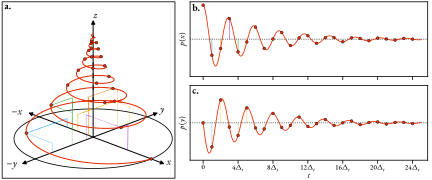
\includegraphics{quadrature_detection/quadrature_detection.pdf}
    \caption[
        An illustration of the free evolution of the bulk
        magnetisation of an ensemble of spin-$\nicefrac{1}{2}$ nuclei
        according to the Bloch model.
    ]{
        \textbf{a.} An illustration of the free evolution of the bulk
        magnetisation of an ensemble of spin-$\nicefrac{1}{2}$ nuclei
        immediately after the application of a $\ang{90}_y$ pulse according to
        the Bloch model.
        The projections of the magnetisation vector onto the
        $x$- and  $y$-axes are plotted in panels \textbf{b.} and \textbf{c.},
        respectively. Modern \acs{NMR} spectrometers utilise quadrature
        detection, such that the $x$- and  $y$- projections of the time-varying
        magnetisation are sampled at regular time intervals, separated by
        $\Dt$.  The resulting \acs{FID} is given by the complex value $p(x) +
        \iu p(y)$.
    }\label{fig:quadrature}
\end{figure}

Everything has now been established to state the Bloch equations, which
describe the evolution of the bulk magnetisation of an ensemble of identical
spin-$\nicefrac{1}{2}$ nuclei in the rotating frame:
\begin{equation}
    \frac{\mathrm{d}\tilde{\symbf{M}}(t)}{\mathrm{d}t} =
    \begin{bmatrix}
        -R_2 & -\Omega & -\gamma B_1 \sin(\phi_{\text{RF}}) \\
        \Omega & -R_2 & \gamma B_1 \cos(\phi_{\text{RF}}) \\
        \gamma B_1 \sin(\phi_{\text{RF}}) & -\gamma B_1 \cos(\phi_{\text{RF}}) & -R_1
    \end{bmatrix}
    \tilde{\symbf{M}}(t)
    + R_1 M_0
    \begin{bmatrix}
        0 \\ 0 \\ 1
    \end{bmatrix},
\end{equation}
\Cref{fig:quadrature}.a depicts the
evolution of an off-resonance bulk
magnetisation vector after the application of an
\ac{RF} pulse with $\phi_{\text{RF}} = \nicefrac{\pi}{2}$, and an appropriate
combination of duration and power to induce a clockwise rotation of \ang{90}
about the $y$-axis; such a pulse is denoted $\ang{90}_{y}$.
Assuming that negligible evolution due to the offset occurs during the pulse,
the magnetisation vector will land on the $x$-axis, and evolve according to
\begin{subequations}
    \begin{gather}
        \tilde{M}_x(t) = M_0 \cos(\Omega t) \exp(-R_2 t),\\
        \tilde{M}_y(t) = M_0 \sin(\Omega t) \exp(-R_2 t),\\
        \tilde{M}_z(t) = M_0 (1 - \exp(-R_1 t)),
    \end{gather}
\end{subequations}
with $t=\qty{0}{\second}$ denoting the time that the magnetisation lands on the
$x$-axis.
During acquisition, the transverse components of the bulk magnetisation are
detected by the spectrometer probe circuitry
(Figures \ref{fig:quadrature}.b and \ref{fig:quadrature}.c), such that the
resulting signal, called the \acfi{FID}, is given by
\begin{subequations}
    \begin{gather}
        y(t) = c \tilde{M}_+(t),\\
        \tilde{M}_+(t) = \tilde{M}_x (t) + \iu \tilde{M}_y (t) = M_0 \exp(\iu \Omega t - R_2 t),
    \end{gather}
\end{subequations}
with $c \in \mathbb{R}_{>0}$ being a proportionality constant.


\subsection{The NMR Spectrometer}

Modern \ac{NMR} spectrometers are capable of conducting a plethora of
experiments which can aide chemists.
In essence, a spectrometer comprises a high-field magnet, a probe, components
which are used to transmit \ac{RF} pulses to the probe, and components which
are used to process the resulting signal from the probe. A brief summary of
these is now given.

\subsubsection{The Magnet}
The static $\symbf{B}_0$ field is generated by a magnet which is composed of a
superconducting solenoid immersed in liquid helium; common materials used for
the solenoid include Nb-Ti alloy and Nb\textsubscript{3}Sn. To minimise the
extent of helium evaporation, the dewar containing the helium is lined with
a thermal radiation shield. The helium dewar is then surrounded by a larger
dewar containing liquid nitrogen,
\correction{which is finally encased in a vacuum chamber.\label{corr:vacuum}}
A bore passes through the $z$-direction of
the magnet, which is maintained at a user-specified temperature. Within the
bore sits the probe as well as the sample. Magnets with high field
strengths are desirable, as both the resolution ($\propto B_0$) and \ac{SNR}
($\propto B_0^{\nicefrac{3}{2}}$) of the data are affected. At the
time of writing, commercial spectrometers which operate at and above a
\proton\ Larmor frequency of \qty{1}{\giga\hertz} (\qty{23.5}{\tesla}) exist,
though these are uncommon and are employed primarily for the study of large
biomolecules
\correction{and solid-state \ac{NMR}\label{corr:solid-state}}.
For most applications, including
the study of small molecules, spectrometers with more modest field strengths on
the order of \qty{100}{\mega\hertz} are typically adequate. Due to their cheap
operating costs and small size, ``benchtop'' \ac{NMR} spectrometers, which
comprise permanent magnets and typically operate on the order of
\qty{10}{\mega\hertz}, have also become popular in educational and
high-throughput settings~\cite{Giberson2021}.

To ensure a high spatial field homogeneity (a necessity for data with
acceptable resolution) a series of coils called \textit{shims} surround the
sample. Each coil produces a weak magnetic field with a specific spatial
profile in accordance with a spherical harmonic function; a collection of shims
can cancel out
\correction{small\label{corr:small-inhomog}}
inhomogeneities inherent to the main magnet.
A field-frequency lock is used to ensure the stability of the
field. The lock is effectively a small \ac{NMR} spectrometer, tuned to a
specified isotope (typically \textsuperscript{2}H\footnote{
    \textsuperscript{2}H-enriched solvents are routinely used to make up
    \ac{NMR} samples. In \proton\ \ac{NMR} experiments, this ensures that an
    extremely intense signal due to the solvent does not dwarf the signals from
    other spins in the sample. This makes \textsuperscript{2}H a suitable
    nucleus to monitor by the lock, as it present in high concentrations, but
    rarely directly studied.
}), which monitors the resonance frequency of the isotope over
time. If the frequency begins to drift, the current in the $Z_0$ coil is
appropriately adjusted, which induces a constant change in field strength
throughout the sample volume.

\subsubsection{The Probe}
\correction{The probe sits inside the bore of the magnet and has a number of
responsibilities including holding the sample, regulating the sample temperature,
and housing the coils used to pulse the sample with \ac{RF}
radiation as well as coils which are used to generate field
gradients\cite[Section 4.7]{Levitt2007}.\label{corr:probe}}
The \ac{RF} coils also receive the response from the sample during detection.
The principle source of data corruption in \ac{NMR} experiments is thermal
noise within the probe circuitry.  For this reason, cryogenic probes have
become a popular development, in which the coils and other probe electronics
are maintained at a very low temperature (typically about
$\qty{20}{\kelvin}$)~\cite{Kovacs2020}.

\subsubsection{The Transmitter}
The transmitter is responsible for the generation of \ac{RF} pulses
with specified power, timing and phase.
A synthesiser acts as an \ac{RF} source, producing a continuous carrier wave at
or very close to the Larmor frequency of the target nucleus. This frequency
($\omega_{\text{RF}}$) can be adjusted in order to determine the center of the
spectrum. The difference between the carrier frequency and the reference
``basic frequency'' of the spectrometer is referred to as the \emph{transmitter
offset} $\foff$.  The output of the synthesiser is gated to ensure pulses are
applied at the desired times. Attenuators/amplifiers then adjust the power
of the pulse, which travels to the probe.

\subsubsection{The Receiver}
During detection, the time-varying current induced in the probe coil by
the sample magnetisation \correction{travels to\label{corr:travel}} a receiver,
which comprises a series of components designed to convert the
analogue current to the digital \ac{FID} which is stored in computer memory.
One of the processes that the receiver is responsible for is \emph{quadrature
detection}~\cite[Section 13.6]{Keeler2010}, which ensures
\acp{FID} are frequency discriminated, i.e. that they possess the requisite
information to determine whether a given component in the \ac{FID} has a
frequency that is above or below the transmitter frequency.
This is achieved by splitting the signal from the probe into two channels. In
each channel, the signal, which is of a very high frequency
(\unit{\mega\hertz}), is mixed with a reference signal of frequency
$\omega_{\text{RF}}$. The mixing process results in a low-frequency
(\unit{\kilo\hertz}) signal being generated, along with a very high frequency
signal. The reference signal in one channel possesses a phase which
is shifted by \ang{90} relative to the other, such that the combined signal
constitutes a quadrature pair.
Both signals are then sent through a low-pass filter to remove
the high frequency component produced through mixing. Finally, an analogue to
digital converter translates the signal to the real and imaginary components of
a binary dataset which constitutes the \ac{FID}.

\subsection{The Structure of the \acs{FID}}
The result of running a \ac{1D} \ac{NMR} experiment is an \ac{FID} $\by \in
\mathbb{C}^N$ which is sampled at equally spaced points in time, with
consecutive samples separated by time $\Dt$:
\begin{equation}
    \begin{gathered}
        \by = \begin{bmatrix}
            y_0 & y_1 & y_2 & \cdots & y_{N-1}
      \end{bmatrix}\T\\
      \equiv
      \begin{bmatrix}
          y(t=0) & y(t=\Dt) & y(t=2\Dt) & \cdots & y(t=(N-1)\Dt)
      \end{bmatrix}\T,
    \end{gathered}
\end{equation}
where $y(t)$ is the (continuous) variation of the generated signal as a
function of time,
and $N$ (often a power of 2) is the number of points sampled. The inverse of
the sampling rate,
$\nicefrac{1}{\Dt}$ is the \correction{\emph{spectral width}\label{corr:sw}} $\fsw$ which
defines how wide the range of samplable frequencies is, in accordance with the
Nyquist theorem~\cite{Shannon1949}.

\acp{FID} adopt the form of a summation of $M \in \mathbb{N}$ complex
exponentials (signals). Each signal will be subjected to damping due to
transverse relaxation, which is typically exponential in nature. An \ac{FID}
therefore takes the form\footnote{
    This provides an idealised model of an \ac{FID}, based on the
    underlying theory of the experiment. In reality, there is the possibility
    of significant deviations from this model being realised. One potential
    cause of this is the influence of magnetic field inhomogeneities, which
    will cause spectral peaks to deviate from having Lorentzian lineshapes
    (\cref{subsec:nmr-proc}). In cases where distortions to the data have
    occurred, techniques such as \emph{reference deconvolution}~\cite{Morris1997}
    can be used as a corrective measure in a bid to make the data agree more
    closely with this model.
}
\begin{subequations}
    \begin{gather}
        y_n = x_n(\bth) + w_n \quad
            \quad \forall n \in \lbrace 0, 1, \cdots, N - 1 \rbrace,
            \label{eq:y=x+w} \\
        x_n(\bth) =
        \sumM \amexpphim \exp\left(
            (2 \pi \iu (f_m - \foff)- \eta_m ) n \Dt
        \right).
        \label{eq:x-1d}
    \end{gather}
    \label{eq:1d}%
\end{subequations}%
\cref{eq:1d} indicates that \iac{FID} comprises contributions from the
(deterministic) evolution of the spin magnetisation $\bx$ and experimental
noise $\bw$ (\emph{vide infra}). Each signal which contributes to $\bx$ is
defined by four parameters:
\begin{itemize}
    \item Amplitude $a \in \mathbb{R}_{>0}$ ,
    \label{pg:param-constraints}
    \item Phase $\phi \in (-\pi, \pi]$ (\unit{\radian}),
    \item Frequency $f \in \left[\hspace*{2pt}\foff - \nicefrac{1}{2} \hspace*{2pt}
        \fsw, \foff + \nicefrac{1}{2} \hspace*{2pt}\fsw \right]$ (\unit{\hertz}),
    \item Damping factor $\eta \in \mathbb{R}_{>0}$ (\unit{\per\second}).
\end{itemize}%
\Iac{FID} can therefore be parameterised by the vector $\bth \in
\mathbb{R}^{4M}$:
\begin{equation}
    \bth =
    \begin{bmatrix}
        \symbf{a}\T & \symbf{\phi}\T & \symbf{f}\T & \symbf{\eta}\T
    \end{bmatrix}\T,
\end{equation}
where $\bda \in \mathbb{R}^M = [a_1 \hspace{2pt} a_2 \hspace{2pt} \cdots
\hspace{2pt} a_M]^{\mathrm{T}}$ is a vector of all amplitudes, $\bdphi \in
\mathbb{R}^M$ is a vector of all phases, etc.
An alternative, more concise, notation for \correction{\cref{eq:x-1d}}
involves the \emph{complex amplitudes} and \emph{signal poles} associated with
the \ac{FID}:
\begin{subequations}
    \begin{gather}
        x_n(\bth) = \sumM \alpha_m^{\vphantom{n}} z_m^n,\\
        \alpha_m = \amexpphim,\\
        z_m = \exp\left(
            \left(2 \pi \iu \left(f_m - \foff\right) - \eta_m\right) \Dt
        \right).\label{eq:signal-pole}
    \end{gather}
    \label{eq:x-alpha-z}%
\end{subequations}
The respective influences of the four parameters on a signal in the time-domain
are depicted in Figures \ref{fig:amp-phase-freq-damp}.a1 to
\ref{fig:amp-phase-freq-damp}.d1.
\begin{figure}
    \centering
    \includegraphics{amp_phase_freq_damp/amp_phase_freq_damp.pdf}
    \caption[
        An illustration of the influence of the four parameters associated
        with a signal in both the time-domain and the Fourier-domain.
    ]{
        An illustration of the influence of the four parameters associated
        with a signal in both the time-domain (a1 to d1) and Fourier-domain
        (a2 to d2).
        The red signal is generated with the same parameters across all panels:
        $a = a_{\text{red}}$, $\phi = 0\,\unit{\radian}$, $f = f_{\text{red}}$,  $\eta =
        \eta_{\text{red}}$.  The blue and yellow signals were produced by
        altering one parameter out of the four.
        \textbf{a.} $a_{\text{yellow}} = \nicefrac{1}{2} a_{\text{blue}} =
        \nicefrac{1}{4} a_{\text{red}}$.
        \textbf{b.}
        $\phi_{\text{blue}} = \nicefrac{\pi}{4}\,\unit{\radian}$,
        $\phi_{\text{yellow}} = \pi\,\unit{\radian}$.
        \textbf{c.}
        $f_{\text{blue}} = \nicefrac{1}{2} f_{\text{red}}$,
        $f_{\text{yellow}} = 0$.
        \textbf{d.}
        $\eta_{\text{yellow}} =
        \nicefrac{1}{2}\eta_{\text{blue}} =
        \nicefrac{1}{4}\eta_{\text{red}}$.
        The real and imaginary components of each signal are plotted, with the
        imaginary component being paler than its real counterpart.
    }
    \label{fig:amp-phase-freq-damp}%
\end{figure}

Multidimensional experiments involve incrementing one or more delays within the
pulse sequence, in order to obtain an array of \ac{1D} \acp{FID}. In a
$D$-dimensional dataset, each contributing signal is parameterised by an
amplitude and phase as before, along with $D$ distinct frequencies and damping
factors, such that a general parameter vector  $\bth \in \mathbb{R}^{2(1+D)M}$
is given by
\begin{equation}
    \bth =
    \begin{bmatrix}
    \symbf{a}\T &
    \symbf{\phi}\T &
    {\bdfone}\T &
    \cdots &
    {\bdfD}\T &
    {\bdetaone}\T &
    \cdots &
    {\bdetaD}\T
    \end{bmatrix}\T,
    \label{eq:theta}
\end{equation}
where $\bdfD$ and $\bdetaD$ are the frequencies and damping factors in the
actively acquired (direct) dimension, and $\lbrace \bdfone, \cdots,
\bdfDminusone \rbrace$ and
$\lbrace \bdetaone, \cdots, \bdetaDminusone \rbrace$ are those for the indirect
dimension(s).
Indirect dimensions can exhibit different forms of evolution, depending on
the precise nature of the pulse sequence, of which two are very
common~\cite[Section 4.3.4]{Cavanagh2007}. \acp{FID} whose constituent signals
evolve according to $\cos(2 \pi f t)$ or $\sin(2 \pi f t)$ modulate the
amplitude of the direct dimension across increments, while those whose signals
evolve according to $\exp(2 \pi \iu f t)$ and $\exp(-2 \pi \iu f t)$ modulate
the phase instead.
For experiments which produce amplitude-modulated \acp{FID},
both the cosine and sine forms should be acquired if possible, as this ensures
that spectra with desirable properties can be generated. The same is true for the positive
and negative forms when phase-modulated \acp{FID} are acquired (\emph{vide
infra}). In general, a $D$-dimensional \ac{FID} $\bY \in \mathbb{C}^{\None
\times \cdots \times \ND}$ can be expressed as
\begin{subequations}
    \begin{gather}
        \ynonenD = \xnonenD(\bth) + \wnonenD,\\
        \xnonenD
            = \sumM \amexpphim \prodD
            \zeta^{(d)}\left(2 \pi \left(f^{(d)}_m  - \foffd\right) \nd \Dtd\right)
            \exp\left(-\eta^{(d)}_m \nd \Dtd\right),\\
        \zeta^{(d)}(\cdot)
        \begin{cases}
            = \exp(\iu\cdot) & d = D \\
            \in \left\lbrace \cos(\cdot), \sin(\cdot), \exp(\iu\cdot) \exp(-\iu\cdot)\right\rbrace & \text{otherwise}
        \end{cases},
    \end{gather}
    \label{eq:general-fid}%
\end{subequations}%

It is typical to assume that the data is corrupted by an array of \ac{AWGN},
i.e. the noise instances are described by a complex normal distribution with
mean 0, and pairs of noise instances are statistically independent, regardless
of their time separation:
\begin{subequations}
    \begin{gather}
        \wnonenD \sim
        \mathcal{N_C}\left(0, 2\sigma^2\right) \\
        \begin{gathered}
            \implies \Re\left(\wnonenD\right) \upmodels \Im\left(\wnonenD\right),\\
             \Re\left(\wnonenD\right) \sim \mathcal{N}\left(0, \sigma^2\right),\\
             \Im\left(\wnonenD\right) \sim \mathcal{N}\left(0, \sigma^2\right). \\
        \end{gathered}
    \end{gather}
\end{subequations}
The extent by which \iac{FID} is corrupted by noise is given by its \ac{SNR},
the ratio of signal power and noise power:
\begin{equation}
    \SNR\left(\bY\right) \coloneq
        \frac{1}{2 N_{\text{tot}} \sigma^2}
        \sum_{\none=0}^{\None-1} \cdots \sum_{\nd=0}^{\ND-1}
        \left \lvert \xnonenD \right \rvert^2,
        \label{eq:snr}
\end{equation}
where $N_{\text{tot}} \coloneq \None \times \cdots \times \ND$ is the total
number of points the \ac{FID} comprises. Due to the large dynamic range
observed for the \ac{SNR} across datasets, it is common to express it using a
logarithmic scale instead, in units of decibels (\unit{\deci\bel}):
\begin{equation}
    \SNR_{\unit{\deci\bel}} \coloneq 10 \log_{10} \left(\SNR\right).
    \label{eq:snr-db}
\end{equation}

\section{An Overview of NMR Data Analysis}
To gain insights from \ac{NMR} experiments on the chemical system of interest,
extraction of the defining parameters $\bth$ is necessary, though the majority
of \ac{NMR} users are unlikely to think about the process of \ac{NMR} analysis
in this way. For example:
\begin{itemize}
    \item An understanding of the chemical environments of atoms in a molecule
        can be gained by considering the chemical shifts of the various peaks
        in the spectra, which are a proxy for the \ac{FID} frequencies
        $\symbf{f}$.
    \item  The relative stoichiometries\note{does this make sense?} of a
        molecule can be elucidated by inspecting the integrals of spectral
        peaks, which are directly related to the \ac{FID} amplitudes $\bda$
\end{itemize}

\note{
    \begin{itemize}
        \item Structure of NMR data
        \item Typical approach to analysing the data (FT, peak pick, integrate, baseline correction, window functions, zero-filling etc),
        \item Estimation techniques: LP, SVD techniques, iterative techniques (AMARES, VARPRO), Bayesian techniques (CRAFT), ML techniques
    \end{itemize}
}

\subsection{Conventional NMR Analysis}

\subsection{Estimation Techniques for NMR Analysis}

\section{Overview of this work}

\subsection{Conception and motivation}
\note{Confirm whether this is accurate with Ali}
The initial motivation for this thesis came from discussions within the NMR
Methodology group in Manchester involving my principal
supervisor Dr. Mohammadali Foroozandeh and coworkers (notably Prof. Gareth
Morris and Prof. Mathias Nilsson) when Dr. Foroozandeh was a Postdoctoral
researcher there. There was an interest in generating pure shift \ac{NMR}
spectra from \acs{2DJ} spectra using an appropriate estimation and
reconstruction algorithm. While little progress was made while Dr. Foroozandeh
was in Manchester, he wished to continue with it after moving to Oxford to take
up a research fellowship. I took on a project with a broader scope
when I joined his nascent research group, starting with developing a routine
and accompanying software for estimating \ac{1D} \acp{FID}. Subsequently, a
number of applications involving \ac{FID} estimation were worked on, including
the original \ac{2DJ} project.

\subsection{Thesis Overview}
This thesis is broken into three principal themes, which span the proceeding
three chapters:
\begin{itemize}
    \item Chapter \ref{chap:theory} discusses the theory behind routines which
        can be applied to determine parameter estimates which describe \ac{1D}
        and \ac{2D} \ac{NMR} datasets.
    \item Chapter \ref{chap:results} provides illustrations of the effectiveness
        of the estimation routine on numerous \ac{NMR} datasets. Furthermore,
        means in which the established estimation routine can be extended for
        useful applications are explored, with these applications being:
        \begin{itemize}
            \item The generation of pure shift spectra with featuring peaks
                with desirable lineshapes from \ac{2DJ} datasets (Section
                \ref{sec:pure-shift}).
            \item Analysis of amplitude-attenuated datasets, such as those
                derived from diffusion and inversion recovery experiments
                (Section \ref{sec:seq}).
            \item Overcoming quadratic phase behaviour and baseline distortions
                associated with excitation by a single \acl{FS} pulse (Section
                \ref{sec:bbqchili}).
        \end{itemize}
    \item Chapter \ref{chap:nmrespy} describes the source code, called
        \acs{EsPy}, which has been written to provide access to the described
        routines presented.
\end{itemize}



\chapter{Theory}
\label{chap:theory}

\begin{chapterquote}{Garth Marenghi, Garth Marenghi's Darkplace}
    The human spirit cannot be overcome. You know, as a writer, if you took away my paper, I would write on my heart. If you take away my ink, I'd write on the wind.\vspace*{1em}\\
    It wouldn't be an ideal way to work.
\end{chapterquote}

This chapter provides a detailed outline of an estimation routine which has
been developed for the parametric estimation of \acp{FID}. \note{More detail?}

\section{Outline of the Problem}
\label{sec:theory-outline}
For the purposes of this work, it is always assumed that an \ac{FID} to be
estimated
$\bY \in \mathbb{C}^{\None \times \cdots \times \ND}$
is hypercomplex in form, meaning that it obeys
\cref{eq:general-fid} with $\zeta^{(d)} = \exp(\iu \cdot)\ \forall d \in
\lbrace 1, \cdots D \rbrace$:
\begin{subequations}
    \begin{gather}
        \ynonenD = \xnonenD(\bth) + \wnonenD,\\
        \xnonenD(\bth) =
        \sumM \amexpphim
        \prodD \exp\left(\left(
            2 \pi \iu \left(f^{(d)}_m - \foffd\right)
            -\eta_m\right)
            \nd \Dtd\right),\label{eq:x}\\
        \wnonenD \sim \mathcal{N_C}\left(0, 2\sigma^2\right),%
    \end{gather}%
    \label{eq:hypercomplex-fid}%
\end{subequations}%
where $\Dtd = \nicefrac{1}{\fswd}$.
Under this model, it is assumed that
\iac{FID} consists of a summation of $M$ damped complex sinusoids in the
presence in \ac{AWGN}.
It is the goal of parametric estimation to establish the
identity of all the quantities which describe the model component $\bX$, which
are distilled into the vector $\bth \in \mathbb{R}^{2(D + 1)M}$, given by
\cref{eq:theta}.
\Cref{eq:x} can be expressed in terms of complex amplitudes and signals poles
as follows:
\begin{subequations}%
    \begin{gather}%
        \xnonenD(\bth) = \sumM \alpha_m \prodD {z^{(d)}_m}^{\nd},\\
        \alpha_m = \amexpphim,\\
        z_m^{(d)} = \exp\left(
            \left(2 \pi \iu \left(f_m^{(d)} - \foffd\right) - \eta^{(d)}_m\right) \Dtd
        \right).%
    \end{gather}%
    \label{eq:x-alpha-z}%
\end{subequations}%
Due to the assumed \ac{AWGN} nature of the noise array, the \ac{pdf} of an
individual noise component is
\begin{equation}
    p(\wnonenD) =
        \frac{1}{2\pi \sigma^2}
        \exp\left( -\frac{\left\lvert \wnonenD \right\rvert^2}{2\sigma^2}\right).
\end{equation}
As the elements are independent and identically distributed, the joint \ac{pdf}
describing the entire noise array is given by the product of each element's
\ac{pdf}:
\begin{equation}
    \begin{split}
        p\left(\bW\right) &=
            \prod_{\none=0}^{\None - 1}
            \cdots
            \prod_{\nD=0}^{\ND - 1}
            \frac{1}{2\pi \sigma^2}
            \exp\left(
                -\frac
                {\left\lvert \wnonenD \right\rvert^2}
                {2\sigma^2}\right) \\
            &= \frac{1}{\left(2\pi \sigma^2\right)^{\mathfrak{N}}}
            \exp\left( -\frac{\left\lVert \bW \right\rVert^2}{2\sigma^2}\right),
    \end{split}
\end{equation}
where $\mathfrak{N} \coloneq \None \times \cdots \times \ND$ is the total
number of points the \ac{FID} comprises.
As the noise array is the difference between the data and model, the
likelihood function of $\bth$ given $\bY$, $\mathcal{L}\left(\bth \vert
\bY\right)$, is
\begin{equation}
    \mathcal{L}\left(\bth \vert \bY\right) =
    \frac{1}{\left(2\pi \sigma^2\right)^{\mathfrak{N}}}
        \exp\left( -\frac{\left\lVert \bY - \bX(\bth) \right\rVert^2}{2\sigma^2}\right).
\end{equation}
It is common to consider instead the log-likelihood function,
$\ell\left(\bth \vert \bY\right)$. As application of the logarithm is a
monotonic transformation, the arguments of the maxima of $\mathcal{L}$ and
$\ell$ are equivalent.
\begin{equation}
    \ell\left(\bth \vert \bY\right) =
        -\mathfrak{N} \ln\left(2 \pi \sigma^2\right)
        -\frac{\left\lVert \bY - \bX(\bth) \right\rVert^2}{2\sigma^2}.
    \label{eq:log-likeihood}
\end{equation}
\Cref{eq:log-likeihood} implies that the optimal set of parameters
$\bth^{(*)}$, often referred to as the \acfi{MLE}\acused{MLE},
is that which minimises the
squared norm of the difference between the data and model, often call the
\acfi{RSS}:
\begin{equation}
    \bthstar = \argmax_{\bth \in \mathbb{R}^{2(D+1)M}}
        \ell\left(\bth \vert \bY\right) \equiv
        \argmin_{\bth \in \mathbb{R}^{2(D+1)M}} \left\lVert \bY - \bX(\bth) \right\rVert^2.
    \label{eq:argmin_y-x}
\end{equation}
The application of \ac{NLP} is a well-established approach to solve such a
problem\cite{Fletcher1987,Nocedal2006}. The basic principle behind \ac{NLP} is
to iteratively explore, in a methodical way, how a function varies with its
arguments. By using information about the function and optionally its
derivatives, such a routine attempts to find a minimum in the function, and
terminates once this has been achieved. While derivative-free approaches to
\ac{NLP} do exist\cite{Nelder1965,Kirkpatrick1983,Powell2009},
in scenarios where the function under consideration has well-defined,
computationally tractable derivatives, the use of these can be valuable to
solving optimisation problems; the problem outlined in
\cref{eq:argmin_y-x} is such an example.

As discussed already, for \ac{NLP} to perform effectively, a large amount of
\textit{a priori} information is typically required, in the form of an initial
guess.
To achieve this, the method employed in this work use the \ac{MPM}, the subject
of the next section.

\section{Generating an Initial Guess: Matrix Pencil Method}
\label{sec:mpm}
\note{Brief introductory text. Mention applications w. citations}

\subsection{1D Matrix Pencil Method}
\label{subsec:mpm}

\begin{remark}
    In contexts where \ac{1D} datasets are considered specifically, the
    redundant dimension index $^{(1)}$ will be neglected for conciseness.
\end{remark}
The \acfi{MPM}, developed by Hua and Sarkar\cite{Hua1990,Hua1990b,Hua1991}, provides a
route to extracting the signal poles of a \ac{1D} dataset, based on the
assumption that the number or oscillators $M$ is known.
To motivate how the \ac{MPM} works, first consider a dataset which is devoid of
noise, given by \cref{eq:x-alpha-z} with $D=1$:
\begin{equation}
    x_n(\bth) = \sumM \alpha_m^{\vphantom{n}} z_m^n,\\
\end{equation}
Consider the Hankel matrix $\Hx \in \mathbb{C}^{(N-L) \times (L+1)}$:
\begin{equation}
    \Hx =
    \begin{bmatrix}
        x_0 & x_1 & \cdots & x_L\\
        x_1 & x_2 & \cdots & x_{L+1}\\
        \vdots & \vdots & \ddots & \vdots\\
        x_{N-L-1} & x_{N-L} & \cdots & x_{N-1}
    \end{bmatrix}.
\end{equation}
This matrix comprises windowed segments of the FID, with each row comprising
the segment shifted to the right by one point relative to the row above.
$L \in \mathbb{N}$ is the \emph{pencil parameter}, which dictates the size of
each window. From $\Hx$, two matrices are defined, $\Hxone$ and $\Hxtwo$,
formed by the removal of the last or first column of $\Hx$, respectively:
\begin{subequations}
   \begin{gather}
        \Hxone =
        \begin{bmatrix}
            x_0 & x_1 & \cdots & x_{L-1} \\
            x_{1} & x_{2} & \cdots & x_{L} \\
            \vdots & \vdots & \ddots & \vdots\\
            x_{N-L-1} & x_{N-L} & \cdots & x_{N-2}\
        \end{bmatrix}, \\
        \Hxtwo =
        \begin{bmatrix}
            x_{1} & x_{2} & \cdots & x_{L} \\
            x_{2} & x_{3} & \cdots & x_{L+1} \\
            \vdots & \vdots & \ddots & \vdots\\
            x_{N-L} & x_{N-L+1} & \cdots & x_{N-1}\\
        \end{bmatrix}.
   \end{gather}
\end{subequations}
These matrices can be deconstructed into the following forms involving matrices
containing the $M$ signal poles and complex amplitudes that the data comprises:
\begin{subequations}
   \begin{gather}
       \Hxone = \symbf{Z}_{\text{L}} \symbf{A} \symbf{Z}_{\text{R}},\\
       \Hxtwo = \symbf{Z}_{\text{L}} \symbf{A} \symbf{Z}_{\text{D}} \symbf{Z}_{\text{R}},\\
       \mathbb{C}^{\left(\None - \Lone\right) \times M} \ni
       \symbf{Z}_{\text{L}} =
       \begin{bmatrix}
           \symbf{1} &
           \symbf{z} &
           \symbf{z}^2 &
           \cdots &
           \symbf{z}^{N-L-1}
        \end{bmatrix}\T,\\
        \mathbb{C}^{M \times L} \ni
        \symbf{Z}_{\text{R}} =
           \begin{bmatrix}
               \symbf{1} & \symbf{z} & {\symbf{z}}^{2} & \cdots & {\symbf{z}}^{L-1}
           \end{bmatrix} ,\\
        \mathbb{C}^{M \times M} \ni
        \symbf{Z}_{\text{D}} = \diag\left(\symbf{z}\right), \label{eq:ZD}\\
        \mathbb{C}^{M \times M} \ni
        \symbf{A} = \diag\left(\symbf{\alpha}\right),\label{eq:A}\\
        \symbf{\alpha} =
        \begin{bmatrix}
            \alpha_1 & \alpha_2 & \cdots & \alpha_M
        \end{bmatrix}\T,\\
        \symbf{z} =
        \begin{bmatrix}
            z_1 & z_2 & \cdots & z_M
        \end{bmatrix}\T.
   \end{gather}
    \label{eq:HX-decomp}
\end{subequations}
The \emph{matrix pencil} $\Hxtwo - \lambda\Hxone$, with $\lambda \in
\mathbb{C}$, can therefore be expressed as
\begin{equation}
    \Hxtwo - \lambda \Hxone = \symbf{Z}_{\text{L}} \symbf{A} \left(
        \symbf{Z}_{\text{D}} - \lambda \symbf{I}_M
    \right) \symbf{Z}_{\text{R}},
\end{equation}
where $\symbf{I}_M \in \mathbb{C}^{M \times M}$ is the identity matrix.
Assuming that the following condition is met:
\begin{equation}
    M \leq L \leq N - M,\label{eq:pencil_condition}
\end{equation}
the rank of the matrix pencil will be $M$. \cref{eq:pencil_condition}
must be obeyed to ensure that both the number of rows and columns of the matrix
pencil are at least $M$. Now consider the case when the scalar $\lambda$ is
equal to one of the signal poles i.e.  $\lambda = z_m\ \forall m \in
\lbrace 1, \cdots, M \rbrace$. The element $[\symbf{Z}_{\text{D}} -
\lambda \symbf{I}_M]_{m,m}$ will be set to $0$, which will lead to the
determinant of the matrix pencil being $0$. The eigenvalues of the matrix
pencil are the solution of the so-called \emph{generalised eigenvalue problem},
and are defined as\cite[Section 7.7]{Golub2013}
\begin{equation}
    \symbf{z} = \left\lbrace
        z \in \mathbb{C} : \det\left(\Hxtwo - z \Hxone\right) = 0
    \right\rbrace
\end{equation}
One means of finding the signal poles is by finding the eigenvalues of the
matrix $\Hxone^+ \Hxtwo^{\vphantom{+}}$. Deriving the corresponding complex
amplitudes can then be achieved by solving the set of linear equations
\begin{subequations}
    \begin{gather}
        \symbf{\alpha} = \symbf{Z}^+ \symbf{x},\\
        \symbf{Z} =
        \begin{bmatrix}
            \symbf{1} &
            {\symbf{z}} &
            {\symbf{z}}^2 &
            \cdots &
            {\symbf{z}}^{N-1}
        \end{bmatrix}\T.
    \end{gather}
    \label{eq:comp-amps}
\end{subequations}
Extraction of the amplitudes, phases, frequencies, and damping factors from the
signal poles and complex amplitudes can then take place:
\begin{subequations}
    \begin{gather}
        \symbf{a} = \left \lvert \symbf{\alpha} \right \rvert,\\
        \symbf{\phi} = \arctan \left(\frac{\Im (\symbf{\alpha})}{\Re(\symbf{\alpha})}\right),\\
        \symbf{f} = \frac{\fsw}{2 \pi} \Im\left(\ln \symbf{z} \right) + \foff, \\
        \symbf{\eta} = -\fsw \Re\left(\ln \symbf{z}\right).
    \end{gather}
\end{subequations}

\subsubsection{Noisy data}
The presence of noise in the signal complicates the process of
determining the $M$ signal poles, as $\Hy$\,---\,$\Hx$'s equivalent with
elements replaced by the noisy data $\symbf{y}$\,---\, is likely to be
full-rank, given by $\min(N - L, L + 1)$. To minimise the influence of noise on
the estimated signal poles, it is necessary to
generate a rank-reduced matrix $\Hytilde$. By employing the \ac{EYM}
theorem\cite[Section~2.2]{Golub2013}, an appropriate matrix is can be obtained
through \ac{SVD} (see \cref{subsec:linear-algebra}):
\begin{subequations}
    \begin{gather}
    \Hytilde =
        \symbf{U}_M^{\vphantom{\dagger}}
        \symbf{\Sigma}_M^{\vphantom{\dagger}}
        \symbf{V}_M^{\dagger},\\
    \mathbb{C}^{(\None - \Lone) \times M} \ni
        \symbf{U}_M^{\vphantom{\dagger}} =
        \begin{bmatrix}
            \symbf{u}_1 &
            \symbf{u}_2 &
            \cdots &
            \symbf{u}_M
        \end{bmatrix},\\
    \mathbb{C}^{(\Lone + 1) \times M} \ni
        \symbf{V}_M^{\vphantom{\dagger}} =
        \begin{bmatrix}
            \symbf{v}_1 &
            \symbf{v}_2 &
            \cdots &
            \symbf{v}_M
        \end{bmatrix},\\
    \mathbb{C}^{M \times M} \ni
        \symbf{\Sigma}_M^{\vphantom{\dagger}} =
        \diag \left( \sigma_1, \sigma_2, \cdots, \sigma_M \right).
    \end{gather}
\end{subequations}
$\sigma_m$ is the $m$ \textsuperscript{th} largest singular value of $\Hy$;
$\symbf{u}_m \in \mathbb{C}^{N - L}$ and $\symbf{v}_m \in
\mathbb{C}^{L+1}$ are the corresponding left and right singular vectors,
respectively. The \ac{EYM} proves that $\Hytilde$ is the closest matrix of rank
$M$ to $\Hy$ in a Frobenius norm sense, i.e.
\begin{equation}
    \Hytilde = \argmin_{\symbf{A}:\ \rank(\symbf{A}) = M} \left \lVert \symbf{A} - \Hy \right \rVert.
\end{equation}
With a rank-reduced matrix produced from the noisy matrix, the signal poles can
then be derived from the eigenvalues of $\Hytildeone^+
\Hytildetwo^{\vphantom{+}}$, where $\Hytildeone$ and $\Hytildetwo$ have the
same relation to $\Hytilde$ as  $\Hxone$ and  $\Hxtwo$ do to  $\Hx$. As a
less expensive alternative, the same result can be achieved by
computing the eigenvalues of $\symbf{V}_{M1}^+\symbf{V}_{M2}^{\vphantom{+}}$,
with
\begin{subequations}
    \begin{gather}
        \symbf{V}_{M1} =
        \begin{bmatrix}
            \symbf{v}_1 & \symbf{v}_2 & \cdots & \symbf{v}_{M-1}
        \end{bmatrix},\\
        \symbf{V}_{M2} =
        \begin{bmatrix}
            \symbf{v}_2 & \symbf{v}_3 & \cdots & \symbf{v}_{M}
        \end{bmatrix}.
    \end{gather}
\end{subequations}
\cref{alg:mpm} provides a pseudo-code description of the \ac{MPM}, while
\cref{lst:mpm} outlines a \Python implementation of it. For optimal
results, the pencil parameter should adhere to $\lfloor \nicefrac{N}{3} \rfloor
\leq L \leq \lfloor\nicefrac{2N}{3}\rfloor$\cite{Hua1990}. In this work,
$\lfloor\nicefrac{N}{3}\rfloor$ is always used, primarily since the computational
complexity of the method is at a maximum when $L = \nicefrac{N}{2}$\footnote{
    With $L = \lfloor\nicefrac{N}{2}\rfloor$, the matrix
    $\symbf{H}_{\symbf{Y}}$ is at its most ``square'' i.e. the number of rows
    and columns are at their most similar. Matrices which are more
    square will increase the demands on computing the \ac{SVD}, with a
    complexity $\mathcal{O}(\min(L+1,N-L+1)^2 \times \max(L+1,N-L+1))$.
}

\begin{algorithm}
    \caption[
        The \acl{MPM}, with the optional prediction of model order using the
        \acl{MDL}.
    ]
    {
        The \acs{MPM}, with the optional prediction of model order using the
        \acs{MDL}, if $M$ is set to $0$.
    }\label{alg:mpm}
    \begin{algorithmic}[1]
        \Procedure{MPM}{$\by \in \mathbb{C}^{N}, \fsw \in \mathbb{R}_{>0}, \foff \in \mathbb{R}, M \in \mathbb{N}_0$}
            \State $L \gets \left\lfloor \nicefrac{N}{3} \right\rfloor$;
            \State $\symbf{H}_{\symbf{y}} \gets
                \begin{bmatrix}
                    y_{0} & y_{1} & \cdots & y_{L}\\
                    y_{1} & y_{2} & \cdots & y_{L+1}\\
                    \vdots & \vdots & \ddots & \vdots\\
                    y_{N-L-1} & y_{N-L} & \cdots & y_{N-1}\\
                \end{bmatrix}
            $;
            \State $\symbf{U}, \symbf{\sigma}, \symbf{V}^{\dagger} \gets
            \SVD(\symbf{H}_{\symbf{y}})$;
            \If {$M = 0$}
                \State $M \gets \operatorname{MDL}(\symbf{\sigma}, L, N)$;
            \EndIf
            \State $\symbf{V} \gets \left[\symbf{V}^{\dagger}\right]^{\dagger}$;
            \State $\symbf{V}_M \gets \symbf{V}\left[:, :M\right]$;
            \Comment{Retain first $M$ right singular vectors.}
            \State $
                \symbf{V}_{M1}, \symbf{V}_{M2} \gets
                \symbf{V}_M\left[:,:M-1\right],
                \symbf{V}_M\left[:,1:\right]
            $;
            \Comment{Remove last/first column}
            \State $\symbf{z} \gets \textsc{Eigenvalues}\left(\symbf{V}_{M1}^+ \symbf{V}_{M2}^{\vphantom{+}}\right)$;
            \State $\symbf{Z} \gets
                \begin{bmatrix}
                    \symbf{1} & \symbf{z} & {\symbf{z}}^2 & \cdots & {\symbf{z}}^{N}
                \end{bmatrix}\T
            $;
            \State $\bdalpha \gets \symbf{Z}^+ \bY$;
            \State $
                \symbf{a} \gets \left\lvert\symbf{\alpha}\right\rvert$;
            \State $\symbf{\phi} \gets \arctan
                \left(\frac{\Im(\symbf{\alpha})}{\Re(\symbf{\alpha})}\right)
            $;
            \State $\symbf{f} \gets \frac{\fsw}{2\pi} \Im \left( \ln \symbf{z} \right) + \foff$;
            \State $\symbf{\eta} \gets -\fsw \Re \left( \ln \symbf{z} \right)$;
            \If {$\symbf{\eta}$ contains negative values}
            \Comment{Purge any oscillators with negative damping}
                \State Remove these from $\symbf{\eta}$, and remove the
                corresponding values from
                $\symbf{a}$, $\symbf{\phi}$, and $\symbf{f}$;
            \EndIf
            \State $\bthzero \gets
                \begin{bmatrix}
                    \symbf{a}\T &
                    \symbf{\phi}\T &
                    \symbf{f}\T &
                    \symbf{\eta}\T
                \end{bmatrix}\T
            $;
            \State \textbf{return} $\bthzero$;
        \EndProcedure
        \Statex
        \Procedure{MDL}{$\symbf{\sigma} \in \mathbb{R}^{L+1}, L \in \mathbb{N}, N \in \mathbb{N}$}
            \State $\operatorname{MDL}_{k-1} \gets \infty$
            \Comment{Ensure that on first iteration ($k=0$), the conditional does not hold}
                \For {$k = 0, \cdots, L$}
                    \State $\operatorname{MDL}_k \gets
                    -\ln\left(
                        \frac
                        {\prod_{r=k}^{L-1} \sigma_{r+1}^{\nicefrac{1}{L-k}}}
                        {\frac{1}{L-k} \sum_{r=k}^{L-1} \sigma_{r+1}}
                    \right)^{(L-k)N}$;
                    \If {$\operatorname{MDL}_k > \operatorname{MDL}_{k-1}$}
                        \State $M \gets k-1$;
                        \State \textbf{break};
                        \Else\State$\operatorname{MDL}_{k-1} \gets \operatorname{MDL}_k$;
                    \EndIf
                \EndFor
                \State \textbf{return} $M$;
        \EndProcedure
    \end{algorithmic}
\end{algorithm}


\subsection{2D Matrix Enhancement and Matrix Pencil Method}
\label{subsec:mmempm}
The \ac{MPM} was extended for the consideration of \ac{2D} data by Hua with the
\acfi{MEMPM}\cite{Hua1992}. The method centers around the enhanced matrix $\EY
\in \mathbb{C}^{\left(\Lone \Ltwo\right) \times \left(\None - \Lone +
1\right)\left(\Ntwo - \Ltwo + 1\right)}$, a block Hankel matrix of the form
\begin{subequations}
    \begin{gather}
        \EY =
        \begin{bmatrix}
            \symbf{H}_{\symbf{Y},0} & \symbf{H}_{\symbf{Y},1} & \cdots & \symbf{H}_{\symbf{Y},\None - \Lone} \\
            \symbf{H}_{\symbf{Y},1} & \symbf{H}_{\symbf{Y},2} & \cdots & \symbf{H}_{\symbf{Y},\None - \Lone + 1} \\
            \vdots & \vdots & \ddots & \vdots \\
            \symbf{H}_{\symbf{Y},\Lone - 1} & \symbf{H}_{\symbf{Y},\Lone} & \cdots & \symbf{H}_{\symbf{Y},\None - 1}
        \end{bmatrix}, \\
        \def\arraystretch{1.3}
        \symbf{H}_{\symbf{Y},\none} =
        \begin{bmatrix}
            y_{ \none, 0 } & y_{ \none, 1 } & \cdots & y_{ \none, \Ntwo - \Ltwo } \\
            y_{ \none, 1 } & y_{ \none, 2 } & \cdots & y_{ \none, \Ntwo - \Ltwo + 1 } \\
            \vdots & \vdots & \ddots & \vdots \\
            y_{ \none, \Ltwo - 1 } & y_{ \none, \Ltwo } & \cdots & y_{ \none, \Ntwo - 1 }
        \end{bmatrix}.
    \end{gather}
\end{subequations}
In a similar fashion to \cref{eq:HX-decomp},
$\symbf{H}_{\symbf{X},\none}$, the noiseless equivalent to
$\symbf{H}_{\symbf{Y},\none}$, can be expressed as
\begin{equation}
    \symbf{H}_{\symbf{X},\none} =
        \symbf{Z}^{(2)}_{\text{L}}
        \symbf{A}
        {\symbf{Z}^{(1)}_{\text{D}}}^{\none}
        \symbf{Z}^{(2)}_{\text{R}}.
\end{equation}
This then enables the noiseless enhanced matrix to be expressed as
\begin{subequations}
    \begin{gather}
        \symbf{E}_{\symbf{X}} =
        \symbf{E}_{\text{L}}
        \symbf{A}
        \symbf{E}_{\text{R}},\\
        \mathbb{C}^{\Lone \Ltwo \times M} \ni
        \symbf{E}_{\text{L}} =
        \begin{bmatrix}
            \symbf{Z}^{(2)}_{\text{L}} \\
            \symbf{Z}^{(2)}_{\text{L}} \symbf{Z}^{(1)}_{\text{D}} \\
            \vdots \\
            \symbf{Z}^{(2)}_{\text{L}} {\symbf{Z}^{(1)}_{\text{D}}}^{\Lone - 1} \\
        \end{bmatrix},\label{eq:EL}\\
        \mathbb{C}^{M \times \left(\None - \Lone + 1\right)\left(\Ntwo - \Ltwo + 1\right)} \ni
        \symbf{E}_{\text{R}} =
        \begin{bmatrix}
            \symbf{Z}^{(2)}_{\text{R}} &
            \symbf{Z}^{(1)}_{\text{D}} \symbf{Z}^{(2)}_{\text{R}} &
            \cdots &
            {\symbf{Z}^{(1)}_{\text{D}}}^{\None - \Lone} \symbf{Z}^{(2)}_{\text{R}} \\
        \end{bmatrix}.
    \end{gather}
\end{subequations}
As was the case in the \ac{1D} \ac{MPM}, \ac{SVD} can be utilised to generate a
filtered matrix $\EYtilde$ with its rank reducd to $M$, in accordance witht he
\ac{EYM} theorem:
\begin{equation}
    \EYtilde =
        \symbf{U}_M^{\vphantom{\dagger}}
        \symbf{\Sigma}_M^{\vphantom{\dagger}}
        \symbf{V}_M^{\dagger}
\end{equation}
If the conditions $\Nd - L^{(d)} + 1 \geq M\ \forall d \in \lbrace 1, 2
\rbrace$ are met, $\range\left(\symbf{U}_M\right) =
\range\left(\symbf{E}_{\text{L}}\right)$. This implies that there is some
nonsingular matrix $\symbf{T} \in \mathbb{C}^{M \times M}$ such that
\begin{equation}
    \symbf{U}_M = \symbf{E}_{\text{L}} \symbf{T}.
\end{equation}
Now consider the following two matrices:
\begin{subequations}
    \begin{gather}
        \symbf{U}_{M1} = \symbf{E}^{\vphantom{(1)}}_{\text{L}1} \symbf{T},\\
        \symbf{U}_{M2} = \symbf{E}^{\vphantom{(1)}}_{\text{L}1} \symbf{Z}^{(1)}_{\text{D}} \symbf{T},\\
        \mathbb{C}^{\Lone \left(\Ltwo - 1\right) \times M} \ni
        \symbf{E}_{\text{L}1} =
        \begin{bmatrix}
            \symbf{Z}^{(2)}_{\text{L}} \\
            \symbf{Z}^{(2)}_{\text{L}} \symbf{Z}^{(1)}_{\text{D}} \\
            \vdots \\
            \symbf{Z}^{(2)}_{\text{L}} {\symbf{Z}^{(1)}_{\text{D}}}^{\Lone - 2}
        \end{bmatrix}.
    \end{gather}
\end{subequations}
$\symbf{U}_{M1}$ and $\symbf{U}_{M2}$ correspond the $\symbf{U}_M$ with the
last and first $\Ltwo$ rows removed, respectively. The matrix pencil for
$\symbf{U}_{M1}$ and $\symbf{U}_{M2}$ can be expressed as
\begin{equation}
    \symbf{U}_{M1} - \lambda \symbf{U}_{M2} =
    \symbf{E}_{\text{L}1} \left( \symbf{Z}^{(1)}_{\text{D}} - \lambda \symbf{I}_M \right) \symbf{T}.
\end{equation}
As seen previously, this matrix structure implies that the elements of
$\bdzone$ are the solutions to the generalised eigenvalue problem, such that
they are the eigenvalues of $\symbf{U}_{M1}^{+} \symbf{U}_{M2}^{\vphantom{+}}$.

To extract the signal poles in the other dimension, $\bdztwo$, the permutation
matrix is defined:
\begin{equation}
    \mathbb{R}^{\Lone \Ltwo \times \Lone \Ltwo} \ni
    \symbf{P} =
    \begin{bmatrix}
        \symbf{e}\left(1\right)\T \\
        \symbf{e}\left(\Ltwo + 1\right)\T \\
        \vdots \\
        \symbf{e}\left(1 + \left(\Lone - 1\right)\Ltwo\right)\T \\
        \symbf{e}\left(2\right)\T \\
        \symbf{e}\left(2 + \Ltwo\right)\T \\
        \vdots \\
        \symbf{e}\left(2 + \left(\Lone - 1\right)\Ltwo\right)\T \\
        \vdots \\
        \vdots \\
        \symbf{e}\left(\Ltwo\right)\T \\
        \symbf{e}\left(2\Ltwo\right)\T \\
        \vdots \\
        \symbf{e}\left(\Lone \Ltwo\right)\T \\
    \end{bmatrix}.
\end{equation}
$\symbf{e}\left(i\right) \in \mathbb{R}^{\Lone \Ltwo}$ corresponds to a unit
vector comprising zeros except for $e_i = 1\ \forall i \in \lbrace 1, \cdots,
\Lone\Ltwo \rbrace$.
Multiplying $\symbf{E}_{\text{L}}$ by the permutation matrix leads to a matrix
in which the roles of the two sets of signal poles are effectively swapped:
\begin{equation}
    \symbf{E}_{\text{LP}} \coloneq \symbf{P} \symbf{E}_{\text{L}} =
    \begin{bmatrix}
        \symbf{Z}^{(1)}_{\text{L}} \\
        \symbf{Z}^{(1)}_{\text{L}} \symbf{Z}^{(2)}_{\text{D}} \\
        \vdots \\
        \symbf{Z}^{(1)}_{\text{L}} {\symbf{Z}^{(2)}_{\text{D}}}^{\Ltwo - 1} \\
    \end{bmatrix}.\label{eq:ELP}
\end{equation}
Note the similarity of \cref{eq:ELP} with \cref{eq:EL}, which
implies that with the same reasoning as given above, $\bdztwo$ can be derived
by extracting the eigenvalues of $\symbf{U}_{M\text{P}1}^+
\symbf{U}_{M\text{P}2}^{\vphantom{+}}$, where $\symbf{U}_{M\text{P}1}$ and
$\symbf{U}_{M\text{P}2}$ correspond to $\symbf{P} \symbf{U}_M$
with the last and first $\Lone$ rows removed, respectively.

In the original account on the \ac{MEMPM}, the final stage involved employing a
pairing algorithm in order to assign the uncorrelated signal poles in $\bdzone$
with $\bdztwo$\cite{Hua1992}. The \emph{modified} \ac{MEMPM} (\acs{MMEMPM}) was
developed in order to overcome two issues with the pairing algorithm: (a) it is
computationally expensive (b) it is prone to return incorrect
pairings\cite{Chen2007}.  As well as the eigenvalues of
$\symbf{U}^{+}_{M1}\symbf{U}_{M2}^{\vphantom{+}}$, the \ac{MMEMPM} requires
extraction of the eigenvectors too, which are contained in the matrix
$\symbf{W}^{(1)}$. Assuming that there are no repeated poles in $\bdzone$, the
correctly paired second set of poles is then generated via
\begin{equation}
    \bdztwo = \diag\left(
        \symbf{W}^{-1}
        \symbf{U}_{M\text{P}1}^+
        \symbf{U}_{M\text{P}2}^{\vphantom{+}}
        \symbf{W}
    \right)
\end{equation}
\note{Talk about case of paired eigenvalues.}

See \cref{alg:mmempm} for a pseudo-code outline, and \cref{lst:mmempm} for a
\Python implementation of the \ac{MMEMPM}.

\subsection{Model Order Selection}
\label{subsec:model-order}
The \ac{MPM} and \ac{MMEMPM} operate under the assumption that the model order
$M$ is known, or at least has been predicted.
It is possible that an individual inspecting the \ac{FID}'s spectrum could
predict $M$ based on the number of peaks visible, however subjective means of
predicting model order are typically viewed as disadvantageous as they have bias
associated with them.
There are various non-subjective criteria which have been established for
estimating the model order of a given signal, with probably the two most
prominent being the \ac{AIC}\cite{Akaike1974} and
\ac{MDL}\cite{Schwarz1978,Rissanen1978}. Both of these consider a family of
potential models which describe a given set of observations, parametrised by
the vector $\bth$. For the purpose of \ac{1D} \ac{FID} estimation, the family
of potential models comprise \cref{eq:x}, with variable $M$. Both the \ac{AIC}
and \ac{MDL} take the same general form:
\begin{equation}
    \mathcal{C}(k) = -c \ln \left(\mathcal{L} \left(\bthstar | \by \right)
    \right) + \mathcal{P}(k) \text{ with } \bthstar \in \mathbb{R}^{4k},
\end{equation}
$\forall k \in \lbrace 0, 1, \cdots \rbrace$. $\mathcal{L} \left(\bthstar |
\by \right)$ is the likelihood
function of a given model, with order $k$, at the \ac{MLE}
$\bthstar$, $c \in \mathbb{R}_{>0}$ is a scaling
constant, and $\mathcal{P}$ is a penalising function, which acts to correct
for bias. As the model order increases, the likelihood function at the \ac{MLE}
will increase in size, as a model with more parameters will be able to fit a
given dataset more accurately. However, as the model order increases, there will
become a point where practically all of the deterministic part of the signal
has been incorporated into the model, and increasing the model order further
leads to the model also accounting for noise. The penalising term, which
is larger for higher $k$, is required in order to estimate a model
order which is parsimonious. Wax and Kailath derived an expression for
the likelihood at the \ac{MLE} for models comprising a summation of
complex sinusoids\cite{Wax1985}\footnote{
    The expression in original paper considers the eigenvalues of the
    covariance matrix for the signal, rather than the singular values of $\Hy$.
    These are equivalent however.
}:
\begin{equation}
    \mathcal{L}\left(\bthstar \in \mathbb{R}^{4k} | \by\right) = \left(
        \frac{
            \prod_{r=k}^{L-1} \sigma_{r+1}^{\nicefrac{1}{L-k}}
        }{
            \frac{1}{L-k} \sum_{r=k}^{L-1} \sigma_{r+1}
        }
        \right)^{(L - k) N},
        \label{eq:wax-pdf}
\end{equation}
$\forall k \in \lbrace 0, 1, \cdots, L - 1 \rbrace$. $\symbf{\sigma} \in
\mathbb{R}^{\Lone}$ is the set of singular values of $\symbf{H}_{\symbf{y}}$,
in decreasing order. The forms of the \ac{AIC} and \ac{MDL} are given by
\begin{subequations}
    \begin{gather}
        \operatorname{AIC}(k) = -2 \ln\left( \mathcal{L} \left(\hat{\bth} | \by\right) \right) + 2k(2 L - k), \\
        \operatorname{MDL}(k) = -\ln\left( \mathcal{L} \left(\hat{\bth} | \by\right) \right) + \tfrac{1}{2} k(2 L - k) \ln N. \label{eq:mdl}
    \end{gather}
\end{subequations}
The \ac{AIC} has been shown to be inconsistent in that it tends to overestimate
the model order as the number of samples increases\cite{Wax1985}. For this
reason, the \ac{MDL} has found greater favour in signal processing
applications. As such, by default the estimation routine employed in this work
utilises the \ac{MDL}:
\begin{equation}
    M = \argmin_{k \in \mathbb{N}_0 :\ k < L} \operatorname{MDL} (k).
\end{equation}
\begin{figure}
    \centering
    \includegraphics{mdl/mdl.pdf}
    \caption[
        A visualisation of the behaviour of the \acs{MDL} for three different
        \acsp{FID} comprising the same deterministic component, but with
        different noise variances.
    ]{
        A visualisation of the behaviour of the \acs{MDL} for three different
        \acsp{FID} comprising the same deterministic component ($\bx$) but
        with different noise instances of differing variances. The model used
        to construct the \acp{FID} features 7
        signals. The three \acsp{SNR} used were
        \qty{7}{\deci\bel} (red), \qty{12}{\deci\bel} (blue), and
        \qty{20}{\deci\bel} (yellow). The \acsp{FID} were generated with $N
        = 256$.
        \textbf{a.} Spectra of the three \acsp{FID}.
        \textbf{b.} The values of the 14 most significant singular values
        associated with the Hankel matrix $\Hy$, with the
        pencil parameter $L$ set to $\lfloor \nicefrac{N}{3} \rfloor =
        85$.
        \textbf{c.} Square points with dotted lines: The negative log-likeliood
        at the \ac{MLE}, i.e. the first term of \cref{eq:mdl}.
        Grey line: the penalty component of the \ac{MDL}, given by the second
        term in \cref{eq:mdl}.
        Circular points with solid lines: the \ac{MDL}.
        Stars denote the minimum of the \ac{MDL} for a given \ac{FID}. The
        \qty{20}{\deci\bel}
        signal is correctly deemed to have a model order of 7, while the other
        two are underestimated (predicted models orders are 5 and 3 for the
        \qty{12}{\deci\bel} and \qty{7}{\deci\bel} \acsp{FID}, respectively).
    }
    \label{fig:mdl}
\end{figure}
Applying the \ac{MDL} for model order selection, and subsequently using the
\ac{MPM} for parameter estimation is the basis of the \ac{ITMPM}\cite{Lin1997}.
\Cref{fig:mdl} illustrates the form of the \ac{MDL} for three signals
with equivalent underlying models, with $M=7$, and noise instances with
different variances. The first 14 singular values of $\Hy$
are plotted in panel b, where it can be seen that beyond the first 7,
which account for signal components, the subsequent singular values, decrease
at a far slower rate. The noise subspace for \acp{FID} with higher \acp{SNR}
have singular values which are (a) smaller in magnitude and (b) more
consistent, such that distinguishing the noise and signal subspaces is an
easier task (cf. the yellow and red lines in panel b). As such, the
\ac{MDL} is more likely to provide a faithful estimate of the true number of
components in the \ac{FID} (panel c) when the \ac{SNR} is higher.

\note{Mention that multidimensional criteria are available, though not
implemented in this work.}

\section{\Acl{NLP}}
\label{sec:nlp}

\subsection{An overview of \ac{NLP}}
\label{subsec:nlp-overview}
In an optimisation problem, the goal is to determine the minimum\footnote{
    In certain applications, the interest could actually be to find the maximum of
    a function. However, it is trivial to transform a maximisation problem into
    a minimisation problem by finding the minimum of negative of the function.
}
of a function $\Fth: \mathbb{R}^n \rightarrow \mathbb{R}, n \in \mathbb{N}$, often
called the \emph{cost function} or \emph{fidelity}.
This is typically with the goal of determining the argument $\bthstar$ at
which the minimum is found:
\begin{equation}
    \bthstar = \argmin_{\bth \in \mathbb{R}^n} \Fth.
    \label{eq:minF}
\end{equation}
The above problem is \emph{unconstrained}, as there are no limitations that the
parameter vector is subjected to. Unless $\Fth$ has particular properties, such
as convexity\footnote{
    A convex function is one such that a line segment through any two points of
    the function lies above it.
}, it is generally only possible to determine a \emph{local} minimum,
rather than a \emph{global} minimum for high-dimensionality problems such as
the one of interest here. $\bthstar$ is a local
minimiser of $\Fth$ if there is a neighbourhood $V \ni \bthstar$ for which
\begin{equation}
    \Fthstar \leq \Fth\ \forall \bth \in V.
  \label{def:local-minimiser}
\end{equation}
$V \subset \mathbb{R}^n$ is a continuous space such that one can move some
amount in any direction away from $\bthstar$ and still be in $V$.
Key to \ac{NLP} are the \emph{necessary conditions}, which define whether a
given vector $\bth$ is a local minimum of the fidelity.
The \emph{first necessary condition} states
that if $\Fth$ is continuously differentiable, and $\bthstar$ is a local extremum\footnote{
    ``Extremum'' is used here instead of ``minimum'', as the first necessary
    condition applies to maxima of a function as well as minima.
} of $\Fth$, then the gradient vector $\bdgthstar \coloneq \nabla \Fthstar$ is the
zero vector:
\begin{equation}
    \bdgthstar = \symbf{0} \in \mathbb{R}^n
\end{equation}
The \emph{second necessary condition} subsequently states that
if $\Fth$ and $\bdgth$ are continuously differentiable, and $\bthstar$ is a
local minimiser of $\Fth$, then the Hessian matrix $\bdHthstar \coloneq
\nabla^2 \Fthstar$ is positive semidefinite, i.e.
\begin{equation}
  \symbf{v}^{\mathrm{T}} \bdHthstar \symbf{v} \geq 0\ \forall \symbf{v} \in \mathbb{R}^n.
\end{equation}
Furthermore, it is a \emph{unique} local minimiser if the \emph{second-order
sufficient condition} is also satisfied, i.e. that the Hessian is positive
definite:
\begin{equation}
    \symbf{v}^{\mathrm{T}} \bdHthstar \symbf{v} > 0\ \forall \symbf{v} \in \mathbb{R}^n.
\end{equation}

A plethora of approaches have been established to determine local minima of
scalar functions. One of the better-known strategies is \emph{Newton's method},
in which a quadratic approximation of the fidelity is considered.
For a given iteration $k \in \mathbb{N}_0$, the fidelity is approximated using
\begin{equation}
    \FQth =
        \Fthk +
        \symbf{h}\T \bdgthk +
        \tfrac{1}{2} \symbf{h}^{\mathrm{T}} \bdHthk \symbf{h},
    \label{eq:quad-approx}
\end{equation}
where $\symbf{h} = \bth - \bthk$.  An updated prediction of the parameter
vector is derived by finding the minimum of this quadratic approximation:
\begin{gather}
    \frac{\partial \Fth}{\partial \symbf{h}} =
        \bdgthk + \bdHthk \symbf{h} \notag\\
    \implies 0 = \bdgthk + \bdHthk \left(\bthkplusone - \bthk\right) \notag\\
    \therefore\ \bthkplusone =
        \bthk - \bdHthk^{-1}
        \bdgthk.\label{eq:newton-update}
\end{gather}
This process is repeated, until the convergence criterion as been met:
\begin{equation}
    \left\lVert \bdgthk \right\rVert \leq \epsilon.
\end{equation}
The convergence threshold $\epsilon > 0$ can be tuned based on the desired
accuracy of the result.
\Cref{eq:newton-update} tends not to be used as the update formula in real
optimisation problems; one of the major downsides of the Newton update is the
possibility that is not a minimising update if the Hessian is not positive
definite. Two primary strategies have emerged which are typically used instead:
\begin{itemize}
    \item \emph{Line search methods}\cite[Chapter 3]{Nocedal2006} determine an
        appropriate direction $\symbf{p}^{(k)}$ along which the updated
        parameter vector is sourced.  After this, an appropriate step length
        $\alpha^{(k)}$ is determined\,---\,typically in an efficient, though not
        optimal manner\,---\,leading to $\bthkplusone = \bthk - \alpha^{(k)}\symbf{p}^{(k)}$.
    \item \emph{Trust region methods}\cite[Chapter 4]{Nocedal2006} define a
        radius $\Updelta^{(k)} > 0$, and determine the minimum of
        \cref{eq:quad-approx} subject to the constraint that
        $\left\lVert\symbf{h}\right\rVert \leq \Updelta^{(k)}$.
\end{itemize}
A trust region method is applied in this work, and as such further
consideration of it will now be made.

\begin{algorithm}
    \caption[
        \acs{NLP} routine employed in this work.
    ]
    {
        \ac{NLP} routine employed in this work. This makes use of
        Algorithms 4.1 \& 7.2 in \cite{Nocedal2006}, with a extra check
        inserted to deal with any negative-amplitude oscillators which may be
        generated as the routine evolves
        (\crefrange{state:neg-amp-start}{state:neg-amp-end}).
    }
    \label{alg:nlp}
    \begin{algorithmic}[1]
        \Procedure {NLP}{$\bY \in \mathbb{C}^{\None \times \cdots \times \ND}, \bthzero \in \mathbb{R}^{2(D + 1)M}$}
            \State $\trustradius{0} \gets \nicefrac{1}{10} \left\lVert \bdgthzeroY \right\rVert$;
            \State $\trmax \gets 16 \trustradius{0}$;
            \For {$k = 0, 1, \cdots $}
            \State $\symbf{p}^{(k)} \gets \textsc{SteihaugToint}\left(\symbf{Y}, \symbf{\theta}^{(k)}, \trustradius{k}\right)$;
                \Comment{See \cref{alg:steihaug-toint}}
                \State $\rho^{(k)} \gets
                    \frac
                        {\Fphithk - \Fphithkpk}
                        {\FphiQthk - \FphiQthkpk}$;
                \If {$\rho_k < \nicefrac{1}{4}$}
                \label{state:decrease-tr-start}
                \State $\trustradius{k+1} \gets \nicefrac{1}{4} \trustradius{k}$;
                    \label{state:decrease-tr-end}
                    \ElsIf {$\rho_k > \nicefrac{3}{4}$ \textbf{ and } $\left\lVert \symbf{p}^{(k)} \right\rVert = \trustradius{k}$}
                \label{state:increase-tr-start}
                \State $\trustradius{k+1} \gets \min\left(2 \trustradius{k}, \trmax\right)$;
                    \label{state:increase-tr-end}
                \Else
                \State $\trustradius{k+1} \gets \trustradius{k}$;
                \EndIf
                \If{$\rho^{(k)} > \nicefrac{3}{20}$}
                \label{state:large-rho-start}
                    \State $\bthkplusone \gets \bthk + \symbf{p}^{(k)}$;
                    \label{state:large-rho-end}
                \Else
                \label{state:small-rho-start}
                    \State $\symbf{\theta}^{(k+1)} \gets \symbf{\theta}^{(k)}$;
                    \label{state:small-rho-end}
                \EndIf
                \If{$k \bmod 25 = 0 \textbf{ and } \symbf{\theta}^{(k+1)}$ contains negative amplitudes}\label{state:neg-amp-start}
                    \State $\symbf{\theta}^{(0)} \gets \symbf{\theta}^{(k+1)}$ with negative-amplitude oscillators removed;
                    \State $\symbf{\theta}^{(*)}, \symbf{\epsilon}^{(*)} \gets \operatorname{NLP}\left(\symbf{Y}, \symbf{\theta}^{(0)}\right)$;
                \EndIf\label{state:neg-amp-end}
                \If{$\left\lVert \bdgthkplusone \right\rVert < \num[print-unity-mantissa=false]{1e-8}$}
                    \State \textbf{break};
                \EndIf
            \EndFor
            \State $\symbf{\theta}^{(*)} \gets \symbf{\theta}^{(k+1)}$
            \State $\symbf{\epsilon}^{(*)} \gets
                \sqrt{
                    \frac
                    {
                        \Fthstar \diag \left(
                            \left[\bdHthstar\right]^{-1}
                        \right)
                    }
                    {(\None \cdots \ND) - 1}
                }$
            \State \textbf{return} $\symbf{\theta}^{(*)}, \symbf{\epsilon}^{(*)}$;
        \EndProcedure
    \end{algorithmic}
\end{algorithm}
The structure of a typical trust region method is presented in
\cref{alg:nlp} (ignoring \crefrange{state:neg-amp-start}{state:neg-amp-end}, which is a custom addition,
see \cref{subsec:phase-variance}). An initial radius for the trust region
$\trustradius{0}$ is defined, along with a maximum permitted radius
$\trmax$, to ensure that excessively adventurous steps do not take place.
For each iteration, a solution to the following sub-problem is sought:
\begin{equation}
    \begin{split}
        \bpk = \argmin_{\bp \in \mathbb{R}^{n}}
            \Fthk +
            (\bthk + \bp)\T \bdgthk +
            \tfrac{1}{2} (\bthk + \bp)\T \bdHthk (\bthk + \bp) \\
        \text{subject to } \left \lVert \bp \right \rVert \leq \trustradius{k}.
    \end{split}
\end{equation}
This sub-problem is not usually minimised exactly, but instead an efficient
means of determining a sufficiently good update is used.
Common approaches include computing the Cauchy point, the Dogleg
method, and a truncated conjugate-gradient
approach commonly called the \ac{ST} method\cite[Chapter 7]{Nocedal2006}.
The latter is employed in this work (see \cref{alg:steihaug-toint} and
\cref{lst:tr}). In the \ac{ST} approach, iterates of the conjugate-gradient
method\cite[Chapter 5]{Nocedal2006} are computed, either until an iterate which
is outside the trust region is computed, or negative curvature is discovered.

Once a provisional update $\bthkplusone = \bthk + \bpk$ is determined using the
\ac{ST} method, a metric is considered which indicates how well the
quadratic estimate agrees with the true value of the fidelity:
\begin{equation}
    \rho^{(k)} = \frac
        {\Fthk - \Fthkpk}
        {\FQthk - \FQthkpk}.
\end{equation}
$\rho^{(k)}$ is the ratio between the actual reduction of the fidelity caused
by taking the proposed step, and the predicted reduction based on the quadratic
model. If $\rho^{(k)}$ is sufficiently close to $1$, the quadratic model being
used to generate new iterates is deemed to be acting well enough to warrant
accepting the proposed update
(\cref{state:large-rho-start,state:large-rho-end}).
Furthermore, if $\rho^{(k)}$ is particularly close to 1, and the proposed
update is at the boundary of the trust radius, it is appropriate to enlarge the
radius of the trust region for the next iteration in an attempt to increase the
rate of convergence
(\cref{state:increase-tr-start,state:increase-tr-end}).
On the other hand, a small value of $\rho^{(k)}$ implies that the
quadratic model reflects the true fidelity poorly, such that the proposed
update should be rejected
(\cref{state:small-rho-start,state:small-rho-end}).
As well as this, the trust region's radius should be
decreased such that the model is more likely to behave faithfully
(\cref{state:decrease-tr-start,state:decrease-tr-end}). In general, the
thresholds which dictate whether to accept an update, and whether to adjust the
trust region radius are customisable. The hard-coded numerical values found in
\cref{alg:nlp} are the values used for the results presented in this work.

\subsection{\acs{NLP} applied to \acs{FID} estimation}
Focus now turns to the specific problem of FID estimation using \ac{NLP}, for
which a general $D$-dimensional dataset will be considered. As established in
\cref{sec:theory-outline}, the fidelity $\FthY : \mathbb{C}^{\None \times
\cdots \times \ND} \times \mathbb{R}^{2(1 + D)M} \rightarrow \mathbb{R}$ is
given by
\begin{equation}
    \FthY = \left \lVert \bY - \bXth \right \rVert^2.
    \label{eq:fidelity}
\end{equation}
The elements of the gradient vector $\bdgthY \in \mathbb{R}^{2(1+D)M}$ and
the Hessian matrix $\bdHthY \in \mathbb{R}^{2(1+D)M \times 2(1+D)M}$ are
derived by taking the first and second partial derivatives of the fidelity with
respect to the elements in $\bth$:
\begin{subequations}
    \begin{gather}
        g_i = -2 \Re
                \left\langle
                    \left(\bY - \bX\right),
                    \frac{\partial \bX}{\partial \theta_i}
                \right\rangle,
        \label{eq:grad} \\
        h_{i,j} = 2 \Re
            \biggl(
                \underbrace{
                    \left\langle
                        \frac{\partial \bX}{\partial \theta_i},
                        \frac{\partial \bX}{\partial \theta_j}
                    \right\rangle
                }_{\circled{1}}
                -
                \underbrace{
                    \left\langle
                        \left(\bY - \bX\right),
                        \frac{\partial^2 \bX}{\partial \theta_i \partial \theta_j}
                    \right\rangle
                }_{\circled{2}}
            \biggl),
            \label{eq:hess}
    \end{gather}
    \label{eq:fidelity-grad-hess}%
\end{subequations}
$\forall i,j \in \lbrace 1, \cdots, 2(1+D)M \rbrace$.
The complete set of first and second derivatives of a particular element of the
model $x \coloneq \xnonenD$, given by \cref{eq:x}, is as follows
$\forall m \in \lbrace 1, \cdots, M \rbrace$,
$\forall d, d^{\prime} \in \lbrace 1, \cdots, D \rbrace$:
\paragraph{First dreivatives}
\begin{subequations}
    \begin{gather}
        \xderiv{\theta_m} \equiv
            \xderiv{a_m} =
            \frac{x}{a_m},
            \label{eq:deriv-a}\\
        \xderiv{\theta_{m + M}} \equiv
            \xderiv{\phi_m} =
            \iu x,\\
        \xderiv{\theta_{m + (d + 1)M}} \equiv
            \xderiv{\fdm} =
            2 \pi \iu \Dtd \nd x,\\
        \xderiv{\theta_{m + (d + D + 1)M}} \equiv
            \xderiv{\etadm} =
            - \Dtd \nd x.
    \end{gather}
    \label{eq:first-derivs}
\end{subequations}
\paragraph{Second derivatives}
\begin{subequations}
    \begin{gather}
        \xderivtwosame{\theta_{m}} \equiv
            \xderivtwosame{a_m} =
            0,
            \label{eq:amp-second-deriv}\\
        \xderivtwodiff{\theta_{m}}{\theta_{m + M}} \equiv
            \xderivtwodiff{a_m}{\phi_m} =
            \frac{\iu x}{a_m},\\
        \xderivtwodiff{\theta_{m}}{\theta_{m + (d + 1)M}} \equiv
            \xderivtwodiff{a_m^{\vphantom{(d)}}}{\fdm} =
            \frac{2 \pi \iu \Dtd \nd x}{a_m},\\
        \xderivtwodiff{\theta_{m}}{\theta_{m + (d + D + 1)M}} \equiv
            \xderivtwodiff{a_m^{\vphantom{(d)}}}{\etadm} =
            \frac{-\Dtd \nd x}{a_m},\\
        \xderivtwosame{\theta_{m + M}} \equiv
            \xderivtwosame{\phi_m} =
            -x,\\
        \xderivtwodiff{\theta_{m + M}}{\theta_{m + (d + 1)M}} \equiv
            \xderivtwodiff{\phi_m^{\vphantom{(d)}}}{\fdm} =
            -2 \pi \Dtd \nd x,\\
        \xderivtwodiff{\theta_{m + M}}{\theta_{m + (d + D + 1)M}} \equiv
            \xderivtwodiff{\phi_m^{\vphantom{(d)}}}{\etadm} =
            -\iu \Dtd \nd x,\\
        \xderivtwodiff{\theta_{m + (d + 1)M}}{\theta_{m + (d^{\prime} + 1)M}} \equiv
            \xderivtwodiff{\fdm}{\fdmp} =
            -4\pi^2 \left(\Dtd \nd \right) \left(\Dtdp \ndp \right) x,\\
        \xderivtwodiff{\theta_{m + (d + 1)M}}{\theta_{m + (d^{\prime} + D + 1)M}} \equiv
            \xderivtwodiff{\fdm}{\etadmp} =
            -2 \pi \iu \left(\Dtd \nd \right) \left(\Dtdp \ndp \right) x,\\
        \xderivtwodiff{\theta_{m + (d + D + 1)M}}{\theta_{m + (d^{\prime} + D + 1)M}} \equiv
            \xderivtwodiff{\etadm}{\etadmp} =
            \left(\Dtd \nd \right) \left(\Dtdp \ndp \right) x,\\
        \xderivtwodiff{\theta_{i}}{\theta_{j}} =
            \xderivtwodiff{\theta_{j}}{\theta_{i}},
            \label{eq:symmetric-second-derivs}\\
        \xderivtwodiff{\theta_{i}}{\theta_{j}} = 0\ \text{ if not specified above.}
        \label{eq:zero-second-deriv}
    \end{gather}
    \label{eq:second-derivs}
\end{subequations}
\Cref{eq:zero-second-deriv} indicates that any second derivative
with respect to two parameters which do not belong to the same oscillator in
then model will always be $0$. This, along with the symmetrical nature of the
second derivatives (\cref{eq:symmetric-second-derivs}) drastically reduces the
required number to explicitly compute, from $4 (1 + D)^2 M^2$ per data-point
to  $(1+D)\left(3 + 2D\right)M$. Finally, \cref{eq:amp-second-deriv}
indicates that another $M$ second derivatives do not need to be computed, as
they are always $0$. See \cref{tab:number-of-derivatives} for the total
number of derivatives that need to be computed for datasets with different
numbers of dimensions.
\begin{table}
    \begin{center}
        \begin{tabular}{ c c c }
            \toprule
            Dimensions &
                \raisebox{\depth}{\#} 1\textsuperscript{st} derivatives &
                \raisebox{\depth}{\#} 2\textsuperscript{nd} derivatives\\
            \midrule
            $1$ & $4M\None$ & $9M\None$\\
            $2$ & $6M\None\Ntwo$ & $20M\None\Ntwo$\\
            $3$ & $8M\None\Ntwo\Nthree$ & $35M\None\Ntwo\Nthree$\\
            $D$ &  $2(1 + D)M \mathfrak{N}$ &  $((1 + D)(3 + 2D) - 1)M \mathfrak{N}$\\
            \bottomrule
        \end{tabular}
    \end{center}
    \caption{
        The number of first and second derivatives that are necessary to
        compute the gradient vector and Hessian matrix of the fidelity for
        1- 2- and 3-dimensional datasets, as well as a general $D$-dimensional
        dataset.
    }
    \label{tab:number-of-derivatives}
\end{table}

\subsection{Approximating the Hessian}
\label{subsec:hess-approx}
Despite many of the model second derivatives being $0$, computation of those
that are not zero, and subsequently using these the form the Hessian matrix,
can be an expensive part of the optimisation routine.
Numerous optimisation problems exist where this is the case, and as such
there is considerable precedent for improving the efficiency of optimisation
algorithms by generating approximations of the Hessian which are demanding to
compute.
Examples include the \ac{GN} method and \ac{LM} algorithm,
which are specifically for \ac{RSS} problems\cite[Chapter
10]{Nocedal2006}, as well as quasi-Newton methods such as the \ac{BFGS}
method\cite[Chapter 6]{Nocedal2006}.

The \ac{GN} and \ac{LM} approaches replace the true Hessian matrix at each
iteration with the following expression:
\begin{equation}
    h_{i,j} = 2 \Re
        \left\langle
            \frac{\partial \bX}{\partial \theta_i},
            \frac{\partial \bX}{\partial \theta_j}
        \right\rangle,
    \label{eq:hess-approx}
\end{equation}
i.e. term \circled{2} in \cref{eq:hess}, which involves the model second
derivatives, is neglected. All that needs to be generated is the Jacobian
$\symbf{J} = \nicefrac{\partial \bX}{\partial \bth}$. This can
bring a very large reduction in the computational cost, as no extra
derivatives need to be computed for the Hessian at all, since the Jacobian is
already required for generating the gradient vector.
In situations where the residuals between the data and model are small, term
\circled{1} will tend to dominate term \circled{2}, and as such these methods
often enjoy a convergence rate which is comparable to that of Newton's method
when close to local minima. Despite this, by invoking this approximation, the
rate of convergence, i.e. the number of iterations required to reach
$\bthstar$, tends to be adversely affected. See \cref{subsec:optim-vis} for an
example of this phenomenon.

\subsection{Visualisation of a simple example}
\label{subsec:optim-vis}
\begin{figure}
    \centering
    \includegraphics{optimisation_visualisation/optimisation_visualisation.pdf}
    \caption[
        A visualisation of the trajectory of a 2-parameter optimisation
        involving a simulated \acs{FID} comprising a single signal.
    ]
    {
        A visualisation of the trajectory of a 2-parameter optimisation
        involving a simulated \acs{FID} comprising a single signal.
        \textbf{a.} \& \textbf{b.} Representations of the signal in
        the time domain and Fourier domain, respectively.
        Black dots: the signal to be estimated $\by$.
        Solid grey line: the model generated
        using the initial guess $\bx \left( \bthzero \right)$.
        Dotted grey line: the model generated using the optimised result, $\bx
        \left( \bthstar \right)$.
        \textbf{c.} A contour plot of the fidelity.
        Blue line: the trajectory of the parameter vector with the true
        Hessian matrix used in computing each update.
        Red line: the analogous trajectory using the Hessian approximation
        in place of the true Hessian.
    }
    \label{fig:optim-vis}
\end{figure}
\Cref{fig:optim-vis} provides a visual example of the application of \ac{NLP}
to estimate a simulated \ac{1D} \ac{FID} comprising a single signal.
The FID was constructed using \cref{eq:general-fid} with $M=1$,
$N = 64$, $\fsw = \qty{5.2}{\hertz}$ ($\Dt \approx
\qty{0.192}{\second}$), and $\foff = \qty{0}{\hertz}$.
The signal was parameterised by $\bth \in \mathbb{R}^4$ comprising $a=1$,
$\phi=\qty{0}{\radian}$, $f=\qty{1}{\hertz}$, $\eta=\qty{0.2}{\per\second}$.
\ac{AWGN} was added to the \ac{FID} to give it \iac{SNR} of approximately
\qty{10}{\deci\bel}. As the visualisation of 5D space is beyond the scope of
this work, only two parameters, the frequency and damping factor, were optimised
from an initial guess $\bthzero$; the amplitude and phase were fixed to
their true values throughout. The initial guess comprised a frequency of
\qty{1.1}{\hertz}, and a damping factor of \qty{0.8}{\per\second}, with the
solid grey lines in panels a \& b denoting the model generated in the time- and
Fourier-domains, respectively. $\bthzero$ was subjected to \ac{NLP} twice. In
the first instance, the exact Hessian matrix, given by \cref{eq:hess} was used
in order to compute each update step, while in the second the Hessian
approximation given by \cref{eq:hess-approx} was used. The initial
radius of the trust region was set to $\nicefrac{1}{10}$ of the gradient norm
($\approx 0.3$), which has a precedent in the literature\cite{Gould2005}. The
trajectories of the parameter vector are denoted by coloured lines in panel c.
In both cases, the \ac{NLP} routine successfully converged at a result $\bthstar$
in agreement with the true frequency and damping factor used to construct the
\ac{FID}. However, it is clear that using the true Hessian matrix (blue)
led to a far better rate of convergence compared with the
approximated analogue (red), which exhibited ``zig-zagging''\footnote{
    This phenomenon is often seen in gradient descent methods, in which each
    update occurs along the opposite direction to the gradient.
}.
14 iterations were required to reach the
convergence criterion $\epsilon \leq \num[print-unity-mantissa=false]{1e-8}$
when the true Hessian was used, while 81 were required for the approximated
case. Despite being an anecdotal example, this highlights that use of the true
Hessian matrix tends to allow a better rate of convergence. However, for
\acp{FID} comprising many signals and far more points, the approximated form
often requires a shorter time to converge overall, especially for \ac{2D}
\acp{FID}, as will be illustrated in \cref{sec:profiling}.

\subsection{Phase Variance Minimisation}
\label{subsec:phase-variance}
\Iac{NLP} procedure tasked with minimising the discrepancy between the model
$\bX$ and the observed data $\bY$ is well-suited to produce an accurate
holistic
representation of the data, assuming a sufficiently large
model order is used. However, as has already been discussed, this is not
necessarily sufficient due to the ill-posed nature of the estimation problem.
It is desirable to produce an estimate which not only achieves a good fit to
the data in \iac{RSS} sense, but which is also in agreement with the process
underpinning the observation. It is for this reason that iterative procedures
typically require significant quantities of prior knowledge, beyond basic
assumptions of the underlying model, in order to produce meaningful estimation
results.  This is also why they are often able to produce results which agree
better with a spectroscopist's conception of what the ``correct'' parameter
estimate should look like, relative to other methods where such detailed
information is not exploited.

While the \ac{MPM} is often able to generate seemingly reasonable parameter
estimates,
one particular feature has been noticed in many of its results:
often, oscillators in the result exhibit spurious phase behaviour.
As has been discussed (\cref{subsec:nmr-proc}),
\ac{NMR} datasets for most experiments comprise signals whose phases
depend on their resonance frequencies to first order. This is routinely
corrected in conventional \ac{NMR} spectral processing, such that all signals
are adjusted to acquire a phase of \qty{0}{\radian}. This feature of the
dataset can be exploited in order to overcome the aforementioned shortcoming of
the \ac{MPM}, through appropriate regularisation of the \ac{NLP} routine.
Assuming that the data has been phase corrected\footnote{
    Rather than rely on the data being phase-corrected, one could envisage
    replacing the phase variance with a term which guides the
    oscillators to adopt a first-order phase relationship. The reason why the
    phase variance has been chosen is two-fold: (i) Applying phase-correction
    to \ac{NMR} data is straightforward and can be automated,
    meaning the user would experience minimal burden. (ii) As will be discussed
    in \cref{sec:filtering}, it is beneficial to have a spectrum comprising
    pure absorption-mode Lorentzians in order to produce frequency-filtered
    ``sub-\acp{FID}'' from the original data, so the data being estimated will
    be phase-corrected anyway.
}, incorporating the variance of oscillator
phases into the fidelity can lead to improved estimation results; examples of
this will be provided later (\cref{sec:evaluation}).
The updated fidelity becomes
\begin{equation}
    \FphithY = \left \lVert \bY - \bXth \right \rVert^2 + \circvar,
    \label{eq:fidelity-phasevar}
\end{equation}
where $\circvar$ is the \emph{circular variance} of the oscillator phases.
Oscillator phases are an example of a circular variable, as all
phases are wrapped within an interval of size 2$\pi$\,\unit{\radian}. Given an
unwrapped phase $\widetilde{\phi} \in \mathbb{R}$, the
corresponding wrapped phase $\phi \in \left( -\pi, \pi \right]$ is given by
\begin{equation}
    \phi = (\widetilde{\phi} + \pi) \bmod 2 \pi - \pi.
    \label{eq:phase_wrap}
\end{equation}
This makes the conventional (linear)
definition of variance, given by
\begin{subequations}
    \begin{gather}
        \Var_{\shortmid}\hspace*{-3pt}\left(\symbf{\phi}\right) =
            \frac{1}{M} \sum_{m=1}^{M} \left(\phi_m - \mu\left(\symbf{\phi}\right)\right)^2, \\
        \mu\left(\symbf{\phi}\right) = \frac{1}{M} \sum_{m} \phi_m,
    \end{gather}
\end{subequations}
unsuitable as a metric to define the variation in phases. Consider as a simple
example a scenario
where there are two oscillators with phases $\widetilde{\bdphi} = \left[ \pi +
\delta\:\:\pi - \delta \right]\T$ for some small $\delta$.
The phase variance is expected to be small as the phases are similar.
However, with the inclusion of wrapping through application of
\cref{eq:phase_wrap}, these phases would actually be set to $\bdphi = \left[
    -\pi
+ \delta\:\:\pi - \delta \right]\T$, and the linear phase
variance would be large. It is therefore apparent that a definition of variance
which accounts for the periodicity of the phases is needed. The circular
variance is defined as\cite[Chapter 3]{Fisher1993}
\begin{subequations}
    \begin{gather}
        [0, 1] \ni \circvar = 1 - \frac{R}{M},\\
        R = \sqrt{c_{\Sigma}^2 + s_{\Sigma}^2}, \\
        c_{\Sigma} = \sum_{m=1}^M \cos \phi_m, \\
        s_{\Sigma} = \sum_{m=1}^M \sin \phi_m.
    \end{gather}
\end{subequations}
$R$ is the length of the resultant vector produced by summing $M$ unit vectors
with angles given by $\bdphi$. In the case that all the vectors have the
same angle, $R=M$, leading to the variance being $0$ as expected. At the other
extreme, with $M$ vectors uniformly separated about the unit circle\,---\,such
that there is an angle of $\nicefrac{2 \pi}{M - 1}$\,\unit{\radian} between all
pairs of adjacent vectors\,---\,the
vectors will perfectly cancel, leading to $R=0$. In this case, the maximum
variance of $1$ is obtained.
The inclusion of the phase variance into the fidelity is one of the
motivating reasons for normalising the data prior to estimation (see
\cref{rem:norm-data}). Since $\circvar$ is constrained to the interval $[0,
1]$, if the data were not normalised it is likely that $\lVert \bY - \bX
\rVert^2$ would dominate $\circvar$ in \cref{eq:fidelity-phasevar}, such that
the influence of the phase variance would be negligible.

The first and second derivatives of the circular variance are required for
the computation of the gradient vector and Hessian matrix, whose updated forms
are
\begin{subequations}
    \begin{gather}
        g_i = -2 \Re
                \left\langle
                    \left(\bY - \bX\right),
                    \frac{\partial \bX}{\partial \theta_i}
                \right\rangle
                + \frac{\partial \circvar}{\partial \theta_i}, \\
        h_{i,j} = 2 \Re
            \biggl(
                    \left\langle
                        \frac{\partial \bX}{\partial \theta_i},
                        \frac{\partial \bX}{\partial \theta_j}
                    \right\rangle
                -
                \underbrace{
                    \left\langle
                        \left(\bY - \bX\right),
                        \frac{\partial^2 \bX}{\partial \theta_i \partial \theta_j}
                    \right\rangle
                }_{\parbox{6em}{\scriptsize{Neglected if approximation used}}}
            \biggl)
            + \frac{\partial^2 \circvar}{\partial \theta_i \partial \theta_j}.
    \end{gather}
\end{subequations}
The derivatives of the phase variance are given by:
\begin{subequations}
    \begin{gather}
        \frac{\partial \circvar}{\partial \theta_i} =
        \begin{cases}
            \frac{1}{RM}
            \left(
                c_{\Sigma} \sin \phi_{i-M} -
                s_{\Sigma} \cos \phi_{i-M}
            \right) & M \leq i < 2M\\
            0 & \text{otherwise}
        \end{cases}\\
        \frac{\partial^2 \circvar}{\partial \theta_i \partial \theta_j} =
        \begin{cases}
            \begin{split}
                \tfrac{1}{RM}\left[
                    \tfrac{1}{R^2}
                    \left(c_{\Sigma} \sin \phi_{i-M}  - s_{\Sigma} \cos \phi_{i-M} \right)^2 \right. \\
                    \left. + c_{\Sigma} \cos \phi_{i-M} + s_{\Sigma} \sin \phi_{i-M}
                    - 1
                \vphantom{\tfrac{1}{RM}}\right]
            \end{split}
            & M \leq i, j < 2M, i = j\\
            \begin{split}
                \tfrac{1}{RM}\left[
                    \tfrac{1}{R^2}
                    \left(c_{\Sigma} \sin \phi_{i-M} - s_{\Sigma} \cos \phi_{i-M} \right) \right.\\
                    \times \left(c_{\Sigma} \sin \phi_{j-M} - s_{\Sigma} \cos \phi_{j-M} \right) \\
                    \left. - \cos\left( \phi_{i-M} - \phi_{j-M} \right)
                    \vphantom{\tfrac{1}{R^2}}
                \right]
            \end{split}
            & M \leq i, j < 2M, i \neq j\\
            0 & \text{otherwise}
        \end{cases}
    \end{gather}
\end{subequations}

The phase variance-regularised fidelity (\cref{eq:fidelity-phasevar}) is
minimised according the unconstrained \ac{NLP} routine described above. It is
therefore possible for oscillators to acquire parameters which are unrealistic
as the optimiser evolves (see \cpageref{pg:param-constraints} for an outline of
the expected ranges that the parameters reside in). With the inclusion of
the variance of oscillator phases, there are situations where oscillators
acquire negative amplitudes. Typically, this occurs when there are
oscillators in the \ac{MPM} result which start out with phases that are far from \qty{0}{\radian}. By acquiring a negative amplitude and a phase close to
\qty{0}{\radian}\,---\,the expected phase of most oscillators in the parameter
set\,---\,little change to the \ac{RSS} term is made, while
$\circvar$ will be reduced. The presence of such oscillators is
undesirable, as they are spurious in the context of phased data. As a
result, the \ac{NLP} routine periodically checks for negative-amplitude oscillators
(\crefrange{state:neg-amp-start}{state:neg-amp-end} in \cref{alg:nlp}). After a
given number of iterations ($25$ is the value given in \cref{alg:nlp})
if any oscillators have acquired negative
amplitudes, these are removed from the model, and the routine continues with a reduced number
of oscillators. While not infallible, this can help to to get rid of excessive oscillators in the
model which do not correspond to true signals in the data. For example, in
scenarios where an overestimate of model order has occurred, noise components
will be incorporated into the \ac{MPM} result. These typically have greater
variability in their phases; often, such oscillators gain negative amplitudes
as the \ac{NLP} routine evolves, leading to unwanted signals being removed and
a more parsimonious result being obtained.

\section{Profiling the \acs{MPM} and \acs{NLP}}
\label{sec:profiling}
The routine described for \ac{FID} estimation involves operations which can be
computationally demanding, with the burden on computational resources
increasing with the number of points in the \ac{FID}, as well as the number of
oscillators in the model. This is the case both in terms of the amount of work
done by the \ac{CPU}, and the amount of \ac{RAM} needed to store all the
required data as the routine runs. For the \ac{MPM}, the most
demanding aspect is \ac{SVD} calculations while for numerical optimisation, it
is generation of the Hessian matrix in each iteration. Detailed accounts of the
computational complexity of the \ac{MPM} and \ac{MMEMPM} have been
presented\cite{Hua1992,Chen2007}.  However, it is useful to consider what the
actual run times of these routines are on a modern computer; a lot of
accounts on the \ac{MPM} are from decades before this work, and so the
run time will have decreased considerably thanks to
improvements in processing power. As an example, the account by Pines a
co-workers from 1997 outlining the \ac{ITMPM} states that a signal comprising
$1024$ points would take about
\qty{4.5}{\minute} to be processed by the \ac{MDL} and \ac{MPM}, using a
\qty{100}{\mega\hertz} \ac{CPU}\cite{Lin1997}. On the system used for all
results generated for this work (see \cref{rem:workstation}) an
equivalent computation takes about \qty{100}{\milli\second}.
\begin{remark}
    \label{rem:workstation}
    All results generated in this work were acquired using a workstation
    featuring a Intel\textregistered\ Core\texttrademark\ i9-10900X \ac{CPU} @
    \qty{3.7}{\giga\hertz}, and \qty{32}{\gibi\byte} of \ac{RAM}.
\end{remark}

To acquire the results presented in this section, third-party \Python profilers
were employed to assess both the line-by-line execution times\cite{LineProf},
and the time-dependent \ac{RAM} usage\cite{MemProf}.

\subsection{The \acs{MPM} and \acs{MMEMPM}}
\begin{figure}
    \includegraphics{mpm_profiling/mpm_profiling.pdf}
    \caption[
        Outlines the run times and peak memory consumption of
        the \acs{1D} \acs{MPM} and \acs{2D} \acs{MMEMPM}.
    ]
    {
        Outlines of the run times and peak memory consumption of
        the \acs{1D} \acs{MPM} and \acs{2D} \acs{MMEMPM}.
        The \acp{FID} that were used to acquire these results are described in
        the main text.
        \textbf{a.} panels are related to the \acs{MPM}, while \textbf{b.}
        panels are related to the \acs{MMEMPM}.
        \textbf{a1.} The amount of time required to compute the \ac{MPM}, as a
        function of number of points. Also plotted is a cubic fit of the
        circular points.
        \textbf{a2.} Peak memory consumption in performing the \ac{MPM} as a
        function of the number of points.
        \textbf{b1.} The run times for computing the \ac{MMEMPM} of
        \acp{FID} with $\None = 64$, and variable $\Ntwo$ and $M$.
        \textbf{b2.} The time required to compute the \ac{SVD} of $\EY$ for the
        $M=40$ \acp{FID}. The solid line is a quadratic fit of the circular
        points, while the dashed line is a quadratic fit of the square points.
        \textbf{b3.} Peak memory consumption in performing the \ac{MMEMPM} for
        the $M=40$ \acp{FID}.
    }
    \label{fig:mpm-profiling}
\end{figure}

A series of synthetic \ac{1D} \acp{FID} were constructed, comprising $10$ evenly-spaced
signals, with a
variable number of time-points $N \in \lbrace 512k \hspace*{2pt} \vert
\hspace*{2pt} k \in \lbrace 1, 2, \cdots, 16 \rbrace \rbrace$.
For each \ac{FID}, the \ac{MPM} routine outlined in \cref{lst:mpm} was
performed 5 times, with a pencil parameter $L = \lfloor
\nicefrac{N}{3} \rfloor$.
The mean complete time to run the \ac{MPM} is plotted as a function
of $N$ in panel a1 of \cref{fig:mpm-profiling}, where it can be seen that for
the larger values of $N$ considered, the \ac{MPM} is computed in approximately
$\mathcal{O}({N}^3)$ time. This is because the rate-limiting step of the
\ac{MPM} is the \ac{SVD} of $\Hy$, whose size is to a very good approximation
$\tfrac{2N}{3} \times \tfrac{N}{3}$\footnote{
    \label{fn:svd-complexity}
    The time complexity for the \ac{SVD} of generic a $m \times n$ matrix is
    $\mathcal{O}(\operatorname{min}(m, n)^2 \cdot \operatorname{max}(m, n))$,
    while the space complexity is $\mathcal{O}(mn)$.
}. For smaller values of $N$, a deviation
away from a cubic relationship is observed;
a fit of a cubic function of the form $aN^3 + b$ to the data satisfying $7 \leq k \leq
16$ is plotted in panel a1 to highlight this behaviour.
This arises because the computation of the complex amplitudes using
\cref{eq:complex-amplitudes} has a comparatively significant run time
relative to \ac{SVD} in the low-$N$ regime;
for a $512$ point signal, the \ac{SVD} of $\Hy$ took up roughly 80\% of the
complete run time, while the computation of the complex amplitudes took up
roughly 20\%. For a 8192 point signal, these percentages had changed to
$>\!\!99\%$ and $<\!\!1\%$, respectively.
For all values of $N$,

The \ac{MPM} was run a sixth time on each generated \ac{FID} in order to assess
the effect of $N$ on the space complexity.
The peak \ac{RAM} consumption is plotted in panel a2 of \cref{fig:mpm-profiling}.
A clear quadratic dependence on consumption is realised as function of $N$,
again in agreement with the expected space complexity of the
\ac{SVD}\footnoteref{fn:svd-complexity}.

A similar study was conducted in consideration of the \ac{MMEMPM}. A
series of \ac{2D} \acp{FID} were simulated, all of which all comprised $\None =
64$. The \acp{FID} possessed values of $\Ntwo \in \lbrace 32k
\hspace*{2pt} \vert \hspace*{2pt} \lbrace 1, \cdots, 16 \rbrace \rbrace$.
With the \ac{MPM}, since a
complete \ac{SVD} of the matrix $\Hy$ is computed, the model order is
irrelevant in dictating the run time (at least when $M \ll N$). This is not the
case for the \ac{MMEMPM}; because the \Python implementation used
(\cref{lst:mmempm}) employs a truncated \ac{SVD} in order to compute only the
first $M$ components of $\EY$, the elected model order will have an impact on
run time.  Therefore, \acp{FID} with different model orders were generated: $M
\in \lbrace 10, 20, 40, 80 \rbrace$.

The \ac{MMEMPM} was repeated 5 times for each \ac{FID}, and the mean run
times for each $\Ntwo$ and $M$ considered is plotted in panel b1 of
\cref{fig:mpm-profiling}.
Only the results for cases where the \ac{MMEMPM} was able to yeild a result in
agreement with the data are presented; for certain \acp{FID} with low
$\Ntwo$ and high $M$, appropriate estimation results could not be yielded as
the constituent signals were too poorly resolved.
While in the high-$N$ regime the \ac{MPM} has a cubic time dependence
on the number of points, the \ac{MMEMPM} can be seen to have an approximately
quadratic complexity regarding $\Ntwo$.
For all combinations of $\Ntwo$ and $M$,
the truncated \ac{SVD} was the most time consuming aspect of the routine,
however other steps have notable run times too. Most of the run time is due to
the following five steps (with the relevant lines in \cref{lst:mmempm} given):
\begin{itemize}
    \item Step 1: Construction of $\EY$. This involves building the Hankel matrices
        $\lbrace \symbf{H}_{\symbf{y},\none} : \none \in \lbrace 0, \cdots, 63
        \rbrace \rbrace$, assigning them to the
        correct locations in $\EY$, and finally converting  $\EY$ to a sparse
        matrix\footnote{
            Truncated \ac{SVD} is only available for sparse matrices in
            \textsc{NumPy}\cite{svds}. Some experimenting was done to determine
            the most efficient means of generating $\EY$ in sparse form, and
            subsequently compute its \ac{SVD}.
            It was determined that constructing $\EY$ using a
            standard \textsc{NumPy} array before converting it to
            \ac{CSR} format\cite{csr} was optimal.
        } (Lines \ref{ln:EY-start} to \ref{ln:sparse1}).
    \item Step 2: Truncated \ac{SVD} of $\EY$ to form $\symbf{U}_M$ (Line \ref{ln:sparse2}).
    \item Step 3: Determining $\bdzone$ and  $\symbf{W}^{(1)}$ by computing the
        \ac{EVD} of $\symbf{U}_{M1}^+ \symbf{U}_{M2}^{\vphantom{+}}$ (Lines
        \ref{ln:poles1-start} to \ref{ln:poles1-end}).
    \item Step 4: Generating the second set of signal poles $\bdztwo$, by
        multiplying $\symbf{U}_M$ by the permutation matrix, and extracting
        the diagonal from matrix $\symbf{G}$, computed using \cref{eq:G} (Lines
        \ref{ln:poles2-start} to \ref{ln:poles2-end}). N.B. The \acp{FID} were
        constructed such that the signal poles were unique on all occasions, so
        the additional treatment of repeated signal poles was not necessary.
    \item Step 5: Computation of the complex amplitudes using
        \cref{eq:complex-amplitudes-2d} (Lines \ref{ln:comp-amps-2d-start} to
        \ref{ln:comp-amps-2d-end}).
\end{itemize}
A comparison of the relative times to perform these steps for a few select
pairings of $M$ and $\Ntwo$ is provided by \cref{tab:mmempm-steps}. It can be
seen that as $M$ increases, the relative amount of time spent performing
\ac{SVD} increases, while the amount of time to generate $\EY$ decreases. This
reflects the greater number of iterations required by
the Rayleigh-Ritz method to produce the desired number of \ac{SVD} components,
while the run time to generate $\EY$ remains fixed.

Interestingly, the plots for a given value of $M$ in panel b1 do not exhibit
consistent quadratic behaviour throughout. After a certain value of $\Ntwo$, a
slight reduction in the gradient of the plots in panel b1 can be observed (cf
the square and circular points). This was found to be caused by the \ac{SVD}
computation, whose run times for the $M=40$ \acp{FID} are plotted in panel b2.
The square and circular points both display quadratic behaviour, though the
exact form of the function which
describes them are different ; both sets of points have been fit to curves of
the form of the form $a\Ntwo^2 + b$. After $\Ntwo$ becomes larger than
roughly $200$, the \ac{SVD} run time appears to enter a new regime in which
subsequent increases in  $\Ntwo$ cause the rate of \ac{SVD} to increase at a
slower rate than was the case previously. The exact reason for this probably
lies in the implementation of the Rayleigh-Ritz algorithm, and has not yet been
ascertained.

The peak \ac{RAM} usage for the $M=40$ \acp{FID} as a function of $\Ntwo$ is
plotted in panel b3, where a quadratic complexity is observed. The variation in
memory consumption barely changes as a function of the model order, since the
peak usage is dependent on the size of $\EY$.

It should be noted that the run time and peak \ac{RAM} consumption will also be
(roughly) quadratically dependent on $\None$, just as with $\Ntwo$, i.e.
increasing  $\None$ for  $64$ to  $128$ would cause all the run times in panel
b1 and peak memory usages in panel b3 to quadruple in value.

\begin{table}
    \begin{center}
        \begin{tabular}{ c c c c c c c }
            \toprule
            $\Ntwo$ &
            $M$ &
            Step 1 &
            Step 2 &
            Step 3 &
            Step 4 &
            Step 5 \\
            \midrule
            64 & 10 & 12.2\% & 60.6\% & 2.9\% & 9.7\% & 13.8\% \\
            64 & 40 & 4\% & 74.6\% & 1.9\% & 8.9\% & 9.6\% \\
            512 & 10 & 22.1\% & 67.2\% & 0.2\% & 3.1\% & 7.2\% \\
            512 & 40 & 7.4\% & 81.9\% & 0.1\% & 1.3\% & 9.4\% \\
            512 & 80 & 3.8\% & 85.8\% & 0.1\% & 0.8\% & 9.4\% \\
            \bottomrule
        \end{tabular}
    \end{center}
    \caption[
        A comparison of the relative times to perform the key steps in the \acs{MMEMPM}.
    ]{
        A comparison of the relative times to perform the key steps in the
        \acs{MMEMPM}, for selected pairings on $M$ and $\Ntwo$. See the main
        text for a description of what each step entails.
    }
    \label{tab:mmempm-steps}
\end{table}

\subsection{Computing the Hessian for \acs{NLP}}

\section{Frequency Filtration}
\label{sec:filtering}
The previous section provides motivation for finding ways to reduce the
number of points in the signal and also the number of oscillators that the
signal contains. This has led to work on a procedure for generating
frequency-filtered ``sub-FIDs'' from the original data. A detailed description
of the filtering procedure is presented in this section.

\subsection{The \acl{VE}}
\label{subsec:ve}
In brief, the filtering procedure  consists taking the \ac{FT} of the \ac{FID},
applying a band-pass filter on the spectral data to discard parts of not being
considered, and returning the spectrum back to the time-domain by an \ac{IFT}.
For a filtered \ac{FID} to be faithfully described by the model of a
summation of damped complex sinusoids, it is necessary that the
spectral peaks of interest lie effectively entirely within the filter
region\footnote{
    Lorentzian lineshapes tend to, but don't reach zero, as the distance from
    the maximum tends to $\infty$\cite{Tang1994}. However, as long as a
    sufficiently wide filtering is employed, the regions of the Lorentzian
    which do not pass through the filter can be assumed to be negligible.
}.
For absorptive Lorentzians, due to their characteristically narrow
linewidths, this is straightforward. However, for broader dispersive
Lorentzians, this is far more challenging. For this reason, generating
a spectrum in which only the real component is retained is desired.
Assuming the data has been phase-corrected, this will produce a
spectrum comprising only absorptive Lorentzians. The \ac{VE} has been employed
here, which has found application in the field of compressed sensing
NMR\cite{Mayzel2014,Golowicz2020,Luo2020}. This is a signal with double the
size as the original \ac{FID}, with the key characteristic that its \ac{FT} has
a real component which is equivalent to its counterpart derived from an
unaltered \ac{FID} (except it has double the points), and an imaginary
component of $0$s. The concept of a virtual echo can be applied to data of any
number of dimensions. However, only \ac{1D} virtual echoes are employed in the
work outlined in this thesis. An account of the \ac{2D} virtual echo is
provided in the Appendix (Section \ref{sec:multidim-ve}.

Assuming that a \ac{1D} \ac{FID} $\by \in \mathbb{C}^N$ is phased, such that
$\bdphi = \symbf{0} \in \mathbb{R}^M$, it can be described by
\begin{subequations}
    \begin{gather}
        y_n = \xi_n (c_n + \iu s_n) + w_n,\\
        \xi_n = \sum_m a_m \exp(-\eta_m n \Dt),\\
        c_n / s_n = \sum_m \cos / \sin(2 \pi f_m n \Dt).
    \end{gather}
\end{subequations}
The frequency-dependence has been decomposed into its real and imaginary
components. With this in mind, a conjugate pair of signals $\symbf{\psi}_{\pm}
\in \mathbb{C}^N$ are defined:
\begin{equation}
    \psi_{\pm,n} = \xi_n (c_n \pm \iu s_n) + w_n \equiv \Re(y_n) \pm \iu \Im(y_n)
\end{equation}
Two vectors $\lbrace \symbf{t}_{1}, \symbf{t}_2 \rbrace \in \mathbb{C}^{2N}$
are constructed using the conjugate pair.
$\symbf{t}_1$ is given by $\symbf{\psi}_+$ padded with zeros from below:
    \begin{equation}
        \symbf{t}_1 = \begin{bmatrix}
            \symbf{\psi}_+ \\ \symbf{0} \in \mathbb{C}^{N}
        \end{bmatrix}.
    \end{equation}
$\symbf{t}_2$ is given by $\symbf{\psi}_{-}$ with its elements in
    reversed order ($\cdot^{{\leftrightsquigarrow}}$), padded with zeros
    from above, and finally subjected to a right circular shift by one
    element ($\cdot^{{\circlearrowright}}$):
    \begin{equation}
        \symbf{t}_2 = \begin{bmatrix}
            \symbf{0} \in \mathbb{C}^{N} \\ \symbf{\psi}_-^{{\leftrightsquigarrow}}
    \end{bmatrix}^{{\circlearrowright}}.
   \end{equation}
The \ac{VE} $\by_{\text{ve}}$ is then given by $\symbf{t}_1 +
\symbf{t}_2$, with the first element divided by $2$, which is equivalent to
\begin{equation}
    \by_{\text{ve}} =
    \begin{bmatrix}
        \Re(y_0^{\vphantom{*}}) &
        y_1^{\vphantom{*}} &
        \cdots &
        y_{N-1}^{\vphantom{*}} &
        0 &
        y_{N-1}^* &
        \cdots &
        y_1^*
    \end{bmatrix}\T.
\end{equation}
As eluded to already, the \ac{FT} of $\by_{\text{ve}}$ produces a spectrum
$\symbf{s}_{\text{ve}}$ such that $\Im\left(\symbf{s}_{\text{ve}}\right) =
\symbf{0}$, with $\Re\left(\symbf{s}_{\text{ve}}\right)$ featuring absorption
Lorentzian peaks.

\subsection{The filtering process}
To filter the spectrum $\symbf{s}_{\text{ve}}$, it is subjected multiplication
with a function which acts as a band-pass filter. An example of a suitable
filter is a \emph{super-Gaussian} $\symbf{g} \in \mathbb{C}^{2N}$ defined by a
central index $c \in \lbrace 0, \cdots, 2N-1 \rbrace$ and a bandwidth  $b \in
\mathbb{N}: b < 2N$ in each dimension:
\begin{equation}
    g_n = \exp \left(-2^{p+1} \left(\frac{n - c}{b}\right)^p\right).
    \label{eq:super-Gaussian-onedim}
\end{equation}
The scalar $p \in \mathbb{R}_{>0}$ dictates the steepness
of the filter at the boundaries, with the function becoming more rectangular
as it increases. It is set to $40$ in this work. Application of the
super-Gaussian filter to $\symbf{s}_{\text{ve}}$
would lead to large sections of the filtered spectrum being $0$. This has an
undesired impact on the \ac{MDL}, as noise that has passed through filter (i.e.
the noise inside the region of interest) will now seem to resemble true signal,
as its amplitude is infinitely greater than the zeroed regions. A massive
over-estimation of model order result due to this. In order to obtain better
results from model order selection, an array of synthetic \ac{AWGN} is
added to the filtered spectrum. To achieve this, a region in
$\symbf{s}_{\text{ve}}$ is specified which contains no discernible signal peaks
(referred to as the \emph{noise region}). The variance of this region
$\sigma^2$ is determined, and used to construct a vector of values sampled from
a normal distribution with mean $0$ and variance $\sigma^2$,
$\symbf{w}_{\sigma^2} \in \mathbb{R}^{2N}$.
The filtered spectrum is then given by
\begin{equation}
    \widetilde{\symbf{s}}_{\text{ve}} = \symbf{s}_{\text{ve}} \odot \symbf{g} + \symbf{w}_{\sigma^2} \odot \left(\symbf{1} - \symbf{g} \right).
    \label{eq:Sve-tilde}
\end{equation}
Note that the noise array's magnitude at each point is attenuated by the value
of the super-Gaussian filter, as a means of ensuring the noise variance remains
consistent across the frequency space.

After filtering, $\widetilde{\symbf{s}}_{\text{ve}}$ is returned to the
time-domain by \ac{IFT}. The \ac{IFT} of a real-valued spectrum generates a
conjugate-symmetric signal, which is also a \ac{VE}. This is sliced so as to
retain the first half, which is the final filtered sub-FID $\widetilde{\by} \in
\mathbb{C}^{N}$:
\begin{subequations}
    \begin{gather}
        \widetilde{\symbf{y}}_{\text{ve}} = \IFT(\widetilde{\symbf{s}}_{\text{ve}}),\\
        \widetilde{\by} = \widetilde{\symbf{y}}_{\text{ve}}[0 : N].
    \end{gather}
    \label{eq:yve-tilde}
\end{subequations}
A summary of the filtering process is provided by Figure \ref{fig:filtering}.
\begin{figure}
     \centering
     \includegraphics{filtering/filtering.pdf}
     \caption[
         An illustration of the filtering procedure applied to a \acs{1D}
         \acs{FID}.
     ]{
         An illustration of the filtering procedure applied to a \ac{1D}
         \ac{FID}.
         \textbf{a.} A \ac{VE} $\by_{\text{ve}}$, with the first and last
         $N$ points coloured red and blue, respectively. The middle of the
         \ac{VE} is magnified to highlight its conjugate symmetry.
         \textbf{b.} The \ac{FT} of the \ac{VE}, $\symbf{s}_{\text{ve}}$.
         The region of interest (orange) and noise region (grey) are denoted.
         \textbf{c.} A super-Gaussian function used as a band-pass filter,
         $\symbf{g}$.
         \textbf{d.} \acs{AWGN} vector to be added to the filtered spectrum.
         The magnitude of the signal at each point is dependent on the
         corresponding super-Gaussian value.
         \textbf{e.} The filtered spectrum $\widetilde{\symbf{s}}_{\text{ve}}$,
         formed by applying the super-Gaussian filter, and adding the noise
         vector.
         \textbf{f.} The \ac{IFT} of the filtered spectrum,
         $\widetilde{\symbf{y}}_{\text{ve}}$, from which the final filtered
         signal $\widetilde{\symbf{y}}$ is obtained by extracting
         the first $N$ points.
     }
     \label{fig:filtering}
\end{figure}

The central index and bandwidth of the super-Gaussian filter function are given
by the following expressions:
\begin{subequations}
    \begin{gather}
        c = \tfrac{1}{2} \left(l_{\text{idx}} + r_{\text{idx}}\right), \\
        b = l_{\text{idx}} - r_{\text{idx}},
    \end{gather}
\end{subequations}
where $l_{\text{idx}}$ and $r_{\text{idx}}$ denote the desired
indices where the filter's left and right bounds are located, respectively.
Array indices can be obtained from the corresponding spectral frequencies
$f^{(d)}_{\unit{\hertz}}$ via
\begin{equation}
    \begin{gathered}
        f_{\text{idx}} =
            \left \lfloor
                \frac
                {
                    \left(2N - 1\right)
                    \left(\fsw + 2 \left(\foff - f_{\unit{\hertz}}\right) \right)
                }
                {2 \fsw}
            \right \rceil \\
        \forall f_{\unit{\hertz}} \in
            \left[\foff - \tfrac{1}{2} \fsw, \foff + \tfrac{1}{2} \fsw\right].
        \label{eq:fidx}
    \end{gathered}
\end{equation}
Conversion from \unit{\partspermillion} to array indices can be achieved by
replacing  $f_{\unit{\hertz}}$ in \eqref{eq:fidx} with
$f_{\unit{\partspermillion}} f_{\text{sfo}}$, where $f_{\text{sfo}}$ is the
transmitter frequency (\unit{\mega \hertz}) and $f_{\unit{\partspermillion}}$
is the frequency expressed as a chemical shift.

\subsubsection{Spectrum slicing}
Thus far, the method described is able to reduce the model order of a given
signal, however the signal still comprises the same number of points. However
it is clear that there are a large number of points outside the region of
interest in $\widetilde{\symbf{s}}_{\text{ve}}$ that do not possess any
meaningful information. Discarding such points will then lead to filtered
\ac{FID} with the same information about the signals of interest, but with
far fewer points. A slicing ratio is defined, $\chi \in \mathbb{R}: \chi>
1$,
which dictates the left and right indices at which the spectrum should be
sliced:
\begin{subequations}
    \begin{gather}
        l_{\text{slice}} =
        \begin{cases}
            c - \left \lfloor \frac{b \chi}{2} \right \rfloor &
            \text{if } \geq 0 \\
            0 & \text{otherwise}
        \end{cases} \\
        r_{\text{slice}} =
        \begin{cases}
            c + \left \lceil \frac{b \chi}{2} \right \rceil &
            \text{if } \leq 2N - 1 \\
            2N - 1 & \text{otherwise}
        \end{cases}
    \end{gather}
\end{subequations}
The filtered spectrum is then sliced accordingly:
\begin{equation}
    \widetilde{\symbf{s}}_{\text{ve,slice}} =
        \widetilde{\symbf{s}}_{\text{ve}} [
            l_{\text{slice}} :
            r_{\text{slice}} + 1
        ].
\end{equation}
Generation of the final sub-\ac{FID} is then achieved in a similar fashion to
before: by performing \ac{IFT}, and retaining the first half of the signal.
It is also necessary to scale the signal by the ratio of the number of points
in the sliced spectrum and it's unsliced counterpart, in order to ensure that
the amplitudes of each signal are unaffected.
\begin{subequations}
    \begin{gather}
        \widetilde{\by} =
            \frac{r_{\text{slice}} - l_{\text{slice}}}{2N}
            \IFT(\widetilde{\symbf{s}}_{\text{ve,slice}})
            [0 : N_{\text{slice}}],\\
            N_{\text{slice}} = \left \lfloor \frac{r_{\text{slice}} - l_{\text{slice}}}{2} \right \rfloor
    \end{gather}
\end{subequations}
The associated sweep width and transmitter offset of the \ac{FID} will have
been altered by this process, and in order to derive accurate frequencies and
damping factors for the sliced signal, it is necessary to determine these. The
corrected values can be computed using
\begin{subequations}
    \begin{gather}
        f_{\text{sw,slice}} = \frac{r_{\text{slice}} - l_{\text{slice}}}{2N - 1} \fsw\\
        f_{\text{off,slice}} = \foff + \frac{\fsw}{2} \left(
            1 - \frac{l_{\text{slice}} + r_{\text{slice}}}{2N - 1}
        \right)
    \end{gather}
\end{subequations}

\section{Summary}
The matrix pencil-based methods described above are well established as
effective procedures for parametric estimation of time-domain signals in a
number of disciplines, including radar detection\cite{Hua1994},
acoustics\cite{TODO}, and \ac{NMR}\cite{Lin1997}, with specific application to
relaxometry being a recently introduced application \cite{Fricke2020,
Wortge2023}. Due to considerable advances computational processing power since
the introduction of the technique, estimates can be acquired from \ac{NMR}
signals in reasonable times. One notable downside of the technique that has
been realised while assessing its effectiveness in parametrising \ac{NMR}
\ac{FID}s is its propensity to return oscillators with unexpected phase
behaviour, especially in scenarios involving resonances with close frequencies.
For this reason, estimating phase-corrected \acp{FID}, using the result of the
\ac{MPM} as an initial guess to feed into a phase-variance penalised \ac{NLP}
routine was proposed as a means of improving parameter estimates. The theory
underpinning the procedure has been explored in this chapter.

The computational burden of running the procedure is large and often
intractable for complete \ac{NMR} signals, which often comprise thousands of
samples, and at least hundreds of contributing resonances. This has been
illustrated through profiling both the \ac{CPU} time and the peak memory
requirements for the \ac{1D} and \ac{2D} methods. \note{Say more when
completed?} For this reason, a method to break \acp{FID} into
frequency-filtered sub-signals, by filtering spectra derived using virtual
echoes, is introduced.  This method enables to formation of signals with far
fewer resonances and samples as compared to the full signal.

Algorithm \ref{alg:1d-2d-summary} provides an overview of the principal steps
involved in the \ac{1D} and \ac{2D} estimation procedures. Detailed algorithms
for each step are presented elsewhere in this text.

\begin{algorithm}
    \begin{algorithmic}[1]
        \caption[
            An overview of the estimation procedure outlined in this work.
        ]{
            An overview of the estimation procedure outlined in this work, for
            the consideration of \ac{1D} and \ac{2D} \ac{NMR} signals.
        }
        \label{alg:1d-2d-summary}
        \Procedure{Estimate$1$D}{$
            \by \in \mathbb{C}^{\None},
            \symbf{r}_{\text{interest}} \in \mathbb{R}^2,
            \symbf{r}_{\text{noise}} \in \mathbb{R}^2,
            M \in \mathbb{N}_0
            $
        }
            \State $\widetilde{\by} \gets \textsc{Filter}1\textsc{D}\left(
                \by,
                \symbf{r}_{\text{interest}},
                \symbf{r}_{\text{noise}}
                \right)
            $;
            \Comment{Algorithm \ref{alg:filter-1d}}
            \If{$M=0$}
                \State $M \gets \textsc{MDL}\left(\widetilde{\symbf{y}}\right)$;
                \Comment{\note{TODO}}
            \EndIf
            \State $\bthzero \gets \textsc{MPM}\left(\widetilde{\by}, M\right)$;
            \Comment{Algorithm \ref{alg:mpm}}
            \State $\bthstar, \symbf{\epsilon}^{(*)} \gets \textsc{NLP}\left(\widetilde{\by}, \bthzero\right)$;
            \Comment{Algorithm \ref{alg:nlp}}
            \State \textbf{return} $\bthstar, \symbf{\epsilon}^{(*)}$;
        \EndProcedure
        \Statex
        \Procedure{Estimate$2$D}{$
            \bY_{\cos} \in \mathbb{C}^{\None \times \Ntwo},
            \bY_{\sin} \in \mathbb{C}^{\None \times \Ntwo},
            \symbf{R}_{\text{interest}} \in \mathbb{R}^{2 \times 2},
            \symbf{R}_{\text{noise}} \in \mathbb{R}^{2 \times 2},
            M \in \mathbb{N}_0
            $
        }
            \State $\widetilde{\bY} \gets \textsc{Filter}2\textsc{D}\left(
                \bY_{\cos},
                \bY_{\sin},
                \symbf{R}_{\text{interest}},
                \symbf{R}_{\text{noise}}
                \right)
            $;
            \Comment{Algorithm \ref{alg:filter-2d}}
            \If{$M=0$}
                \State $M \gets \textsc{MDL}\left(\widetilde{\bY}[:, 0]\right)$;
                \Comment{Run the MDL on the first direct-dimension slice.}
            \EndIf
            \State $\bthzero \gets \textsc{MMEMPM}\left(\widetilde{\bY}, M\right)$;
            \Comment{Algorithm \ref{alg:mmempm}}
            \State $\bthstar, \symbf{\epsilon}^{(*)} \gets \textsc{NLP}\left(\widetilde{\bY}, \bthzero\right)$;
            \Comment{Algorithm \ref{alg:nlp}}
            \State \textbf{return} $\bthstar, \symbf{\epsilon}^{(*)}$;
        \EndProcedure
    \end{algorithmic}
\end{algorithm}

Having established an estimation routine, the next chapter focusses on its
performance, as well as applications which are possible through parametric
estimation.


\chapter{Results and Applications}

\section{\acs{1D} Datasets}

In order to assess the estimation routine proposed in Chapter \ref{chap:theory}
-- specifically the effectiveness of applying \ac{NLP} using an initial guess
generated using the \ac{MPM} -- a series of synthetic \acp{FID} were constructed
using \eqref{eq:hypercomplex-fid}. For each \ac{FID}, a model order of $M=20$
was used, the number of points sampled was $\None = 1024$, the sweep width
was $\fswone=\qty{125}{\hertz}$, and the transmitter offset was $\foffone =
\qty{0}{\hertz}$.  Each oscillator was assigned a phase of \ang{0}, while the
amplitudes, frequencies and damping factors were drawn at random from the
following distributions:
$\bdam \sim \mathcal{U}(1, 5)$, $\bdfonem \sim \mathcal{U}(\qty{-55}{\hertz},
\qty{55}{\hertz})$, $\bdetaonem \sim \mathcal{U}(\qty{2}{\per\second},
\qty{8}{\per\second})\ \forall m \in \lbrace 0, \cdots, 19\rbrace$. An extra
constraint was applied to the frequencies,
such that no two oscillators were permitted to have frequencies that differed
by less than $\nicefrac{4 \fswone}{\None} \approx \qty{0.49}{\hertz}$. Each
noiseless \ac{FID} was then corrupted with \ac{AWGN}, with a target \ac{SNR} of
\qty{25}{\deci\bel}\note{Reference that this is the lowest
SNR that the MPM considered to be effective}. The spectra of the simulated
\acp{FID} are presented in panel a of Figure \ref{fig:mpm_vs_nlp}.

For each \ac{FID}, the \ac{MPM} was performed, assuming that the model order is
30, constituting a considerable over-fit. Simulated signals typically show a
clean division between signal and noise components, with noise components
commonly being characterised by small amplitudes and/or very small damping
factors. For this reason, prior to subjecting the \ac{MPM} result to \ac{NLP},
oscillators which satisfied either $\bdam < 0.1$ or  $\bdetaonem <
\qty{0.7}{\per\second}$ were removed from the parameter set. The individual
oscillators which make up the \ac{MPM} result after purging are displayed in panel b of
Figure \ref{fig:mpm_vs_nlp}, along with the residual between the data and the
model.

It can be seen that in several spectral regions across the datasets, especially
those which are more crowded, oscillators possess parameters which deviate
significantly from the true parameters (the true set of oscillators is
presented in panel d), with the most notable feature being individual
oscillator phases, which can stray far from \ang{0}.
The central motivation behind employing phase variance-regularised \ac{NLP} is
as a means of attempting to overcome this detrimental feature of the \ac{MPM}.
It should be noted however, that the \ac{MPM} invariably generates a model with
good agreement with the data, as evidenced by the residual.
In Figure \ref{fig:mpm_vs_nlp}, the blue oscillators are those which agree very
closely with a particular oscillator in the true set of parameters. Oscillators
with other colours are in disagreement for some reason (\textit{vide infra}).
The goal of the \ac{NLP} routine is therefore to adjust the parameters
describing the non-blue oscillators in panel b such that they agree with
oscillators found in the true set, while not affecting the blue oscillators.
The results of \ac{NLP} at convergence ($\epsilon = \num{1e-8}$) are provided
in panel c. ...

\note{Maybe define the notion of a ``frequency neighbourhood''?
    A small rage of frequencies within which it is necessary for the MPM to generate at least the same number of oscillators as the true number for NLP to have a chance of correctly estimating the dataset.
}

\paragraph{Green oscillators}
These oscillators belong to a grouping of oscillators with similar frequencies
which exhibited significant deviation from the true parameter set, but which
were mapped to agree closely with the true result thanks to the \ac{NLP}
routine.

\paragraph{Orange oscillators}
Orange oscillators are examples of scenarios where the \ac{MPM} routine
over-fit a particular spectral region, and the \ac{NLP} routine was able to
purge these excessive oscillators, leading to a parsimonious set of parameters.

\paragraph{Red oscillators}
These oscillators are examples of a cases where the routine has underfit the
dataset, because there are a pair of similar-frequency oscillators in the true
parameter set which were not be individually resolved. In these cases, the
\ac{MPM} assigned only a single oscillator to fit the spectral region, making
it impossible for the \ac{NLP} routine to make any improvements to the
estimation result.

\paragraph{Yellow oscillators}
Similar to red oscillators, yellow oscillators eventually lead to the
under-fitting of the dataset. However, in these cases, the \ac{MPM} has
generated sufficient oscillators in the frequency neighbourhood. Unlike in
scenarios which is seen for the green oscillators though, the \ac{NLP} routine
evolves such that at least one of the oscillators is driven by the phase
variance constraint to acquire a negative amplitude, such that it is purged
from the parameter set. This typically occurs when an oscillator has an initial
phase close to \ang{180}.

\paragraph{Purple oscillators}
The arise rather infrequently, and correspond to over-fits of the dataset.


\begin{sidewaysfigure}
    \centering
    \includegraphics{mpm_vs_nlp/mpm_vs_nlp.pdf}
    \caption[
        The result of estimating a series of 5 simulated signals comprising 20
        oscillators, using solely the \acs{MPM} and also with phase
        variance-regularised \acs{NLP} afterwards.
    ]{
        The result of estimating a series of 5 simulated signals comprising 20
        oscillators (see the main text for details on how the datasets were constructed).
        \textbf{a.} Spectra of the datasets generated.
        \textbf{b.} Plots of spectral lines for each oscillator generated using
        the \acs{MPM}.
        \textbf{c.} An equivalent plot for the result after applying \acs{NLP},
        with the \ac{MPM} result being the initial guess.
        \textbf{d.} Spectral lines corresponding to the true set of oscillators
        used to generate each the datasets.
        Also included in \textbf{b.} -- \textbf{d.} is the residual between the
        data and the sum of the oscillator peaks (grey line).
        The colouring of oscillator lines is described in the main text.
    }
    \label{fig:mpm_vs_nlp}
\end{sidewaysfigure}

\section{\acs{2D} Datasets}
\label{sec:twodim}

\section{Pure-Shift Spectra via \acl{2DJ} Estimation}
\label{sec:pure-shift}

Two key features which the \ac{NMR} community is constantly seeking to improve
are the sensitivity and resolving power of experiments. There are
numerous means of improving spectral sensitivity, via technological
advancements including the production of superconducting magnets with higher
field strengths\note{CITE?} (sensitivity $\propto B_0^{\nicefrac{7}{4}}$),
and cryogenic probes\cite{Kovacs2005}, as well as simply increasing the number
of scans (\ac{SNR} $\propto \text{NS}^{\nicefrac{1}{2}}$).  There are however
few means of achieving better resolution beyond increased field strengths
(resolution $\propto B_0$). Significant interest has therefore been
given to the development of homodecoupled (``pure shift'')
experiments\cite{Meyer2013,Adams2014,Zangger2015}, in which the
effects of homonuclear scalar couplings are removed from the data. The presence
of J-couplings, indicating the close proximity of spins in a chemical
bonding sense, is a distinguishing feature of \ac{NMR}, and is often valuable for
structural assignment. However, in many cases their effect can lead to spectra
which are too crowded for meaningful insights to be gleamed.  Heteronuclear
couplings, between spins with different nuclei (i.e. \proton\ and \carbon) are
straightforward to decouple at the point of \ac{FID} acquisition, using well
known schemes such as WALTZ-16\cite{Shaka1983a, Shaka1983b} and
GARP\cite{Shaka1985}. Homonuclear decoupling is anything but simple on the
other hand.

In this section, an overview of the key techniques which have
been developed to generate pure shift spectra is given, starting with \ac{2DJ}
spectroscopy and finishing up with \ac{PSYCHE}, widely considered the most
robust pure shift experiment in terms of sensitivity and tolerance to strong
coupling. Subsequently, a new technique for generating pure shift spectra via
parametric estimation, named \acf{CUPID} is presented.

\subsection{An Overview of Pure Shift NMR}

\subsubsection{The \acl{2DJ} Experiment}
The \ac{2DJ} experiment\cite{Aue1976, Morris2009} provided the first means of
achieving pure shift spectra.  It has a simple pulse sequence, presented in
Figure \ref{fig:pure_shift_seqs}.a: after excitation of magnetisation onto the
transverse plane, the indirect dimension evolution consists of a spin echo, with
acquisition following immediately afterwards. Fourier transformation in both
dimensions leads to a spectrum in which only scalar couplings contribute in
$\Fone$, as the chemical shifts are refocussed by the spin echo, while both
scalar couplings and chemical shifts contribute in $\Ftwo$.
Peaks belonging to a particular multiplet lie along a line at \ang{45} to the
$F^{(1)}$ and $F^{(2)}$ axes, as seen in panel a. of Figure
\ref{fig:jres_spectrum}.
\begin{figure}%
    \centering%
    \includegraphics{jres_spectrum/jres_spectrum.pdf}%
    \caption[
        Example of a simple \acs{2DJ} spectrum derived from an AMX spin system.
    ]
    {%
        \textbf{a.} Contour plot of an absolute value mode \ac{2DJ} spectrum for an
        AMX spin system, produced by applying sine-bell apodisation on a hypercomplex
        \ac{FID} before a \ac{FT} in both dimensions. Each multiplet lies a
        long a line at \ang{45} to the $F^{(1)}$ and $F^{(2)}$ axes. Note that
        this line often appears to make an angle that is greater than \ang{45}
        with the $F^{(2)}$ axis when viewing spectra, since typically $\fswone
        \ll \fswtwo$. Above the \ac{2DJ} spectrum is a plot of its summation
        along the $\Fone$ axis.
        \textbf{b.} Spectrum generated after application of a \ang{45} shear,
        with its $\Fone$ summation above.
   }%
    \label{fig:jres_spectrum}%
\end{figure}%

An FID generated by the \ac{2DJ} experiment is hypercomplex, taking the form of
\eqref{eq:general fid} with $D=2$ and $\zeta = \exp(\iu\cdot)$, i.e.
\begin{equation}%
    \begin{split}%
        \jresfid\idxnonentwo =
        \sum_{m=0}^{M-1} \bdam \exp\left( \iu \bdphim \right)
            \exp\left(\left(2 \pi \iu \bdfonem - \bdetaonem\right) {\none}_{\vphantom{t}} \Dtone\right) \times \\
            \exp\left(\left(2 \pi \iu \bdftwom - \bdetatwom\right) {\ntwo}_{\vphantom{t}} \Dttwo\right)
            + \symbf{W}\left[n^{(1)}, n^{(2)}\right].
    \end{split}%
    \label{eq:jres-fid}
\end{equation}%
A major downside of the \ac{2DJ} experiment is there is no means of generating
a pair of phase- or amplitude-modulated signals which are the
conventional route to frequency-discriminated spectra with absorption mode
lineshapes. In many multidimensional experiments, changing the phase of
certain \ac{RF} pulses or the use of \acp{PFG} can induce a change in the \ac{CTP},
generating such signal-pairs, though this unavailable with \ac{2DJ}
spectroscopy as no mixing time exists. The FT of $\jresfid$ produces a spectrum
$\jresspec$ with ``phase-twist'' peaks, which possess contributions from both absorption
and dispersion Lorentzians. There are two primary steps involved in obtaining a
pure shift spectrum from $\jresspec$:
\begin{enumerate}
    \item Perform a \ang{45} shear (often called a tilt) on the spectrum array,
        leading to the separation of chemical shifts and scalar couplings onto
        orthogonal axes  (panel b. in Figure \ref{fig:jres_spectrum}). Each
        slice in $\Ftwo$ is subjected to a right circular rotation such that
        \begin{subequations}
            \begin{gather}
                \jresspectilt\left[{\none}\vpsub{\mathrm{sw}},{\ntwo}\vpsub{\mathrm{sw}}\right] =
                \jresspec\left[{\none}\vpsub{\mathrm{sw}},\ntwonew\right],\\
                \ntwonew = \left(
                    {\ntwo}\vpsub{\mathrm{new}} + \left\lfloor
                        \frac
                            {\fswone \Ntwo\vpsub{\mathrm{sw}}}
                            {\fswtwo \None\vpsub{\mathrm{sw}}}
                        \left(
                            \frac{\None\vpsub{\mathrm{sw}}}{2} - \none
                        \right)
                    \right\rceil
                \right) \bmod \Ntwo.
            \end{gather}
        \end{subequations}
        This achieves the mapping $\jresspec\left(\fone,\ftwo\right)
        \rightarrow \jresspec\left(\fone, \ftwo - \fone\right)$.  It should be
        noted that the effectiveness of the shear is maximised when both
        $\nicefrac{\fswtwo}{\fswone}$ and $\nicefrac{\Ntwo}{\None}$ are powers
        of 2\note{check this}.
    \item Sum the spectrum along $\Fone$:
        \begin{equation}
            \specps\idxntwo =
            \sum_{\none=0}^{\None-1} \jresspectilt\idxnonentwo.
        \end{equation}
\end{enumerate}%
Shearing and summing $\jresspec$ actually leads to the absorptive and dispersive
components of the spectrum cancelling each other out . It is necessary to display
the spectrum in absolute value mode before carrying out the above steps (i.e.
use $\Re(\lvert \jresspec \rvert)$).
This still leads to undesirable pure shift spectra with broad ``wings'' on
account of the presence of dispersive character. The dispersive component can
be suppressed by appropriate processing to make the FID envelope symmetric in
both dimensions, such as with sine-bell
apodisation\cite[Section3.3.5]{Lindon1980}, or pseudo-echo
reshaping\cite{Bax1981}, though this results in a significant reduction in
sensitivity being incurred.

\begin{figure}
    \centering
    \includegraphics{pure_shift_sequences/pure_shift_sequences.pdf}
    \caption[
        The pulse sequences of some common pure shift experiments.
    ]{
        \note{Work needed. Figure out the correct delays in ZS, BIRD, PSYCHE}
        The pulse sequences of four of the most common pure shift experiments.
        \textbf{a.} \acs{2DJ}.
        \textbf{b.} The \acs{ZS} method.
        \textbf{c.} The \acs{BIRD} method.
        \textbf{d.} The \acs{PSYCHE} method.
    }
    \label{fig:pure_shift_seqs}
\end{figure}

\subsubsection{The \acl{ZS} Method}
\label{subsec:ZS}
In 1997 Zangger and Sterk introduced a pulse sequence element which achieves
slice-selective excitation, by applying a low \ac{RF} power (weak) \ang{180}
pulse\footnote{Conventionally, a R-SNOB pulse is used\cite{Kupce1995}.} in the
presence of a \ac{PFG} along the $z$-axis\cite{Zangger1997}. Such an element
excites a
given spin only in a narrow range of heights in the sample, as the \ac{PFG}
induces a shift in resonance frequency according to $\Delta \omega(z) = \gamma
G_z z$, where $G_z$ is the magnitude of the \ac{PFG}. By placing a hard
\ang{180} pulse adjacent to the selective pulse, the
``active'' spin in a given slice is rotated by \ang{360} (i.e. no net
rotation), while all other (``passive'') spins are only rotated by \ang{180}.
Placing such a element in the middle of the $\tone$ evolution therefore
achieves refocussing of the J-couplings associated with the active
spin\cite{Aguilar2010}. In order to achieve effective decoupling of any given
pair of spins, it is necessary that the bandwidth of the selective π-pulse is
smaller than the difference in their chemical shifts. However, with more
selective pulses, a smaller proportion of the available spin magnetisation will
contribute to the final FID, and hence sensitivity will be diminished
\footnote{
    The reduction in sensitivity is $\propto \nicefrac{f_B}{\gamma G_z l_z}$,
    where $f_B$ is the selective pulse bandwidth, and $l_z$ is the length of
    the sample lying within the receiver coil ($\approx
    \qty{1.5}{\centi\meter}$).
}.
There is therefore a trade-off between effective decoupling of all spins, and
achieving the greatest sensitivity possible. In the case of strong coupling,
the \ac{ZS} method tends to perform poorly relative to other options for this
reason. The \ac{ZS} element has been applied by Keeler and Pell in order to
generate \ac{2DJ} datasets comprising phase-modulated pairs, enabling the
generation of pure absorption-mode spectra\cite{Pell2007}.


\subsubsection{The \acs{BIRD} Method}
The \ac{BIRD} pulse sequence element\cite{Garbow1982,Bax1983}, presented in
Figure \ref{fig:pure_shift_seqs}.c, also takes advantage of the idea of
selectively inverting passive spins, while leaving active spins unaffected.
However the active spins are those which are directly bound to
\textsuperscript{13}C nuclei, which naturally occur with an abundance of 1.1\%,
while the passive spins are those bound to far more abundant
\textsuperscript{12}C nuclei. The reduction in sensitivity of the experiment
relative to a full-sensitivity experiment is therefore known and constant
across samples. In scenarios where is this strong coupling, \ac{BIRD} can
achieve improved sensitivity over \ac{ZS}, since with the latter a very weak
selective pulse would be required to ensure it is of a sufficiently small
bandwidth. The \ac{BIRD} method is particularly attractive in scenarios where
the sensitivity penalty due to the involvement of a low-abundance nucleus has
already been paid, for example in a \ac{HSQC} experiment\cite{Paudel2013}.

\subsubsection{PSYCHE}
\label{subsec:psyche}
\note{TODO}
Original paper\cite{Foroozandeh2014}, tutorial paper\cite{Foroozandeh2018}, PSYCHE-2DJ\cite{Kiraly2017}.

\subsubsection{Pure Shift NMR via J-Resolved Post-Processing}

There have been previous descriptions of acquiring pure-shift spectra from
typical \ac{2DJ} datasets via more sophisticated post-processing methods.
Nuzillard presented \ac{ALPESTRE}\cite{Nuzillard1996}, in which the parameters
of each indirect-dimension FID are estimated using linear prediction, such that
there is a set of parameters $\symbf{\Theta} \in \mathbb{R}^{\Ntwo \times 4M}$
with
\begin{equation}
    \symbf{\Theta}\left[\ntwo\right] =
    \begin{bmatrix}
        \left[\bda_{\ntwo}\right]\T &
        \left[\bdphi_{\ntwo}\right]\T &
        \left[\bdfone_{\ntwo}\right]\T &
        \left[\bdetaone_{\ntwo}\right]\T
    \end{bmatrix}.
\end{equation}
The parameters generated are used to propagate each FID backward into
$-\tone$, producing a ``full-echo'':
\begin{equation}
    \begin{split}
        \symbf{Y}_{\text{full}}\left[\none, \ntwo\right] = \sum_{m=0}^{M-1}
            \bda_{\ntwo} \left[ m \right]
            \exp\left(\iu \bdphi_{\ntwo} \left[ m \right] \right)
            \exp\left(\left(2 \pi \iu \bdfone_{\ntwo} \left[ m \right] \none
            -\bdetaone_{\ntwo} \left[ m \right] \left\lvert \none \right\rvert \right)\Dtone\right) \\
        \forall \none \in \mathbb{Z}: -\None < \none < \None,\\ \forall \ntwo \in \mathbb{N}_0: \ntwo < \Ntwo.
    \end{split}
\end{equation}
\ac{FT} of generates a spectrum whose real component comprises absorption-mode
Lorentzian character in both dimensions. This opens up the means of producing
pure-shift spectra from the \ac{2DJ} experiment with sharp lineshapes and
without sensitivity loss. A similar approach proposed by Mutzenhardt et al.
instead constructed full echoes via \ac{LP} of each direct-dimension
\ac{FID}, and generation of a full echo by propagating
into $-\ttwo$\cite{Mutzenhardt1999}.

\subsection{An outline of \acs{CUPID}}
\ac{CUPID} aims to generate pure shift spectra by utilising the result of
parametric estimation on \ac{2DJ} data, assumed to take the functional form of
\eqref{eq:jres-fid}.
Instead of estimating successive \ac{1D} \acp{FID}, as has been described by
Nuzillard and Mutzenhardt et al., the entire \ac{2DJ} signal is estimated as a
whole, giving access to the parameter vector $\bth \in \mathbb{R}^{6M}$. Using
$\bth$, a synthetic \ac{1D} \ac{FID}, named the ``\ang{-45} signal'' (Figure
\ref{fig:neg-45}), is produced:
\begin{equation}
    \symbf{y}_{\ang{-45}}\left(\bth\right)\left[ \ntwo \right] =
        \sum_{m=0}^{M-1} \bdam \exp \left(\iu \bdphim \right)
        \exp\left(
            \left(
                2 \pi \iu \left(\bdftwom - \bdfonem\right)
                - \bdetatwom
            \right) \ntwo \Dttwo
        \right).
    \label{eq:neg-45}
\end{equation}
$\forall \ntwo \in \lbrace 0, \cdots, \Ntwo - 1 \rbrace$. The \ang{-45} signal
takes the same functional form as a typical \ac{1D}
\ac{FID} acquired by a pulse-acquire experiment, except that the frequency of
each oscillator, which would usually be $\ftwo$, is replaced with $\ftwo -
\fone$. In a \ac{2DJ} experiment, $\fone$ corresponds to the displacement of a
given oscillator from the central frequency of the multiplet it is associated
with. As such, the oscillators belonging to a given multiplet all provide
a contribution with the same frequency to the \ang{-45} signal, namely the
chemical shift of relevant spin.
\begin{figure}
    \centering
    \includegraphics{neg_45_signal/neg_45_signal.pdf}
    \caption[
        An illustration of the reasoning behind the name ``\ang{-45}
        signal''.
    ]{
        An illustration of the reasoning behind the name ``\ang{-45}
        signal''. The pale red dots denote a typical \ac{2DJ} \ac{FID}, where
        the amount and rate of sampling in the direct dimension is greater than
        in the indirect dimension (i.e. $\None \ll \Ntwo$ and $\fswone \ll
        \fswtwo$). The bright red dots correspond to the first direct-dimension
        signal $\bY_{\text{2DJ}}(0, \ttwo)$, which has the same form as
        \iac{FID} from a pulse-acquire experiment. A hypothetical signal
        generated by propagating the \ac{FID} into $-\tone$, with the same rate
        of sampling in both dimensions, is denoted with pale blue dots. Taking
        the diagonal of this signal, such that it forms a \ang{-45} to the
        $\ttwo$ axis, yields an \ac{FID} $\by_{\ang{-45}}$  which is
        homodecoupled. It should be noted that there is a slightly discrepancy
        between \eqref{eq:neg-45} and this description, in that the
        indirect-dimension damping factors $\bdetaone$ are neglected in the
        former case.
    }
    \label{fig:neg-45}
\end{figure}

\subsubsection{Multiplet Prediction}
A holistic \ac{2D} estimation of the \ac{FID} provides access to other useful
information about the dataset. One such example is the grouping of oscillators
in account of which multiplet structure they belong to. As has already been
established, for oscillators which are associated with the same multiplet
structure, the quantity $\ftwo - \fone$ should be equal. This provides a
criterion in order to assess whether it is likely that two oscillators in the
estimation result belong to the same multiplet:
\begin{equation}
    \left \lvert
        \left( \bdftwo \left[ m_1 \right] -
        \bdfone \left[ m_1 \right] \right) -
        \left( \bdftwo \left[ m_2 \right] -
        \bdfone \left[ m_2 \right] \right)
    \right \rvert < \epsilon
\end{equation}
$\forall m_1, m_2 \in \lbrace 0, \cdots, M-1 \rbrace$, with  $\epsilon \in
\mathbb{R}_{>0}$ being a suitable threshold to account for error in the
estimation. An appropriate value for $\epsilon$ would appear to be half the
spectral resolution in the more poorly resolved dimension, i.e.
$\epsilon = \min\left(\nicefrac{\fswone}{2 \None}, \nicefrac{\fswtwo}{2\Ntwo}\right)$. In situations involving real \ac{2DJ}
signals however, it is found that $\epsilon$ sometimes has to be increased to
values slightly larger than this to achieve effective groupings (\textit{vide
infra}). Algorithm \ref{alg:mp-assign} provides a routine that can be used for
multiplet prediction.

\note{Removal of spurious oscillators}

\subsubsection{Filtration of \ac{2DJ} data}
Unlike the direct-dimension, which can often comprise sparsely distributed
peaks in the Fourier domain, the indirect dimension of \ac{2DJ} datasets tends
to be rather densely populated. As such, it is typically of little use in
attempting to generate filtered sub-\acp{FID} in the indirect dimension. The
filtering procedure utilised for \ac{2DJ} data is therefore an extension of the
filtration procedure for \ac{1D} data described in Section \ref{sec:filtering}
(Figure \ref{fig:jres-filtering}). The filtering procedure involves the
following steps:
\begin{enumerate}
    \item The signal $\symbf{Y}_{\text{ve}} \in \mathbb{C}^{\None \times 2 \Ntwo}$ is
    constructed, such that a virtual echo is formed from each direct-dimension
    signal:
    \begin{equation}
        \begin{split}
            \symbf{Y}_{\text{ve}} \left[n^{(1)}\right] =
                &\left[
                \begin{matrix}
                    \Re\left(\symbf{Y}\left[n^{(1)}, 0\right]\right) &
                    \symbf{Y}\left[n^{(1)}, 1\right] &
                    \cdots
                \end{matrix}\right.
                \\
                &\left.
                \begin{matrix}
                    \symbf{Y}\left[n^{(1)}, \Ntwo - 1\right] &
                    0 &
                    \symbf{Y}\left[n^{(1)}, \Ntwo - 1\right]^* &
                    \cdots &
                    \symbf{Y}\left[n^{(1)}, 1\right]^*
                \end{matrix}
                \right]
        \end{split}
    \end{equation}
    $\forall n^{(1)} \in \lbrace 0, \cdots, N^{(1)} - 1 \rbrace$.
    \item $\symbf{Y}_{\text{ve}}$ is subjected to \ac{FT} along the direct
        dimension to produce the spectrum  $\symbf{S}_{\text{ve}}$ (panel a of
        Figure \ref{fig:jres-filtering}). This has a imaginary component of
        zeros.
    \item A super-Gaussian $\symbf{G} \in \mathbb{R}^{\None \times 2 \Ntwo}$ is
        constructed (panel b):
        \begin{equation}
            \symbf{G} = \symbf{1} \otimes \symbf{g}^{(2)},
        \end{equation}
        where $\symbf{1} \in \mathbb{R}^{\None}$ is a vector of ones, and
        $\symbf{g}^{(2)}$ is a super-Gaussian vector given by
        \eqref{eq:super-Gaussian-onedim} with $d=2$.
    \item A matrix of additive noise is generated by extracting the variance
        $\sigma^2$ of a strip of $\symbf{S}_{\text{ve}}$ which is devoid of
        peaks, and generating an array $\symbf{W}_{\sigma^2} \in
        \mathbb{R}^{\None \times 2 \Ntwo}$ with values independently sampled
        from a normal distribution with mean $0$ and variance  $\sigma^2$.
    \item The spectrum is filtered according to \eqref{eq:Sve-tilde}, yielding
        $\widetilde{\symbf{S}}_{\text{ve}}$ (panel d).
    \item $\widetilde{\symbf{S}}_{\text{ve}}$ is subjected to \ac{IFT} and is
        slicing in half in the direct dimension, yeilding the final filtered
        signal $\widetilde{\symbf{Y}}$:
        \begin{equation}
            \widetilde{\symbf{Y}} = \IFT^{(2)}\left(\widetilde{\symbf{S}}_{\text{ve}}\right) \left[:, : \Ntwo\right].
        \end{equation}
\end{enumerate}

\begin{figure}
    \centering
    \includegraphics{jres_filtering/jres_filtering.pdf}
    \caption[
        An illustration of the filtering procedure for \ac{2DJ} data.
    ]
    {
        An illustration of the filtering procedure for \ac{2DJ} data.
        For each panel is a heat-map of the full \ac{2D} signal, as well as a
        plot underneath of the first slice of the signal in the direct
        dimension.
        \textbf{a.} The spectrum $\symbf{S}_{\text{ve}}$,
        \textbf{b.} Super-Gaussian filter $\symbf{G}$,
        \textbf{c.} Additive noise, attenuated by the super-Gaussian, $\symbf{W}_{\sigma^2} \odot (\symbf{1} - \symbf{G})$,
        \textbf{d.} Filtered spectrum $\widetilde{\symbf{S}}_{\text{ve}}$
        Panels \textbf{a.}--\textbf{d.} are analogous to panels \textbf{b.}--
        \textbf{e.} in Figure \ref{fig:filtering} for the \ac{1D} case.
    }
    \label{fig:jres-filtering}
\end{figure}

\subsection{Results Using \acs{CUPID}}
\label{subsec:cupid-results}
A number of examples of the application of \ac{CUPID} are now provided.
Initially, a few results are presented using data simulated using the Spinach
MATLAB\textregistered\ library\cite{Hogben2011}.
After this, examples are provided with experimental data. In a couple of these,
comparison of the result acquired using \ac{CUPID} is compared with a spectrum
acquired using \ac{PSYCHE}.

For additional details relating to generation of the simulated datasets, see
section \ref{sec:simulated-datasets} in the Appendix.

\subsubsection{``Four Multiplets''}
\begin{figure}
    \centering
    \includegraphics{four_multiplets/four_multiplets}
    \caption[
        The result of applying \acs{CUPID} to 5 instances of simulated
        \acs{2DJ} datasets with 4 heavily overlapping multiplet structures.
    ]{
        The result of applying \ac{CUPID} to 5 instances of simulated \ac{2DJ}
        datasets with 4 heavily overlapping multiplet structures.
        \textbf{a.} Black: pure shift spectrum generated by \ac{CUPID}.
        Grey: \ac{1D} spectrum simulated with Spinach, using the same spin
        system as was used to produce the \ac{2DJ} dataset, but with all scalar
        couplings sets to \qty{0}{\hertz}. This has been offset slightly for
        clarity.
        \textbf{b.} \ac{1D} spectrum of the dataset.
        \textbf{c.} Multiplet structures predicted, using a threshold $\epsilon
        = \nicefrac{\fswtwo}{2 \Ntwo} \approx \qty{0.49}{\hertz}$.
        \textbf{d.} Contour plot of the \ac{2DJ} spectrum in absolute-value
        mode. Coloured points denote the frequencies of oscillators in the
        estimation result.
        Coloured vertical lines denote the predicted central frequencies of
        each multiplet structure.
    }
    \label{fig:four-multiplets}
\end{figure}
A series of simulated \proton\ \ac{2DJ} datasets were generated such that
within a known region of the spectrum, four ddd multiplet structures with
significant overlap existed. To achieve this, a spin-system with 7 spins was
formed, with the spins divided into 2 subsets:
\begin{itemize}
    \item 4 of the spins (the ``estimated spins'') were assigned random
        resonance frequencies sampled from $\mathcal{U}(\qty{-20}{\hertz},
        \qty{20}{\hertz})$.
    \item The remaining 3 spins (the ``coupling spins''), were coupled to each
        of the estimated spins, with the values of the couplings randomly
        sampled from $\mathcal{U}(\qty{-10}{\hertz}, \qty{10}{\hertz})$.  The
        coupling spins were given chemical shifts such that they lay far from
        the estimated spins in the spectrum (i.e. their frequencies were $\gg
        \qty{20}{\hertz}$).
\end{itemize}
\ac{AWGN} noise was added to the \ac{FID}, with a target \ac{SNR} of \qty{30}{\deci\bel}.
A filtered sub-\ac{FID} containing only the signals from the estimated spins
was then generated using the filtering procedure described above, with
$l^{(2)}_{\unit{\hertz}} = \qty{30}{\hertz}$,
$r^{(2)}_{\unit{\hertz}} = \qty{-30}{\hertz}$, and
$\xi = 1.1$. The resulting sub-\ac{FID} was expected to comprise 32 ($4 \times
2^3$) oscillators. To assess the estimation procedure's ability, a random
integer from the range 33 -- 40 was selected as the initial number of
oscillators. Hence, the initial guess from the \ac{MMEMPM} would comprise an
excessive number of oscillators. The \ac{FID} was subjected to
estimation, yielding the result vector $\bthstar$. Spurious oscillators were
checked for, using the criteria outlined above, with the threshold for
multiplet assignment set to half the spectral resolution in the direct
dimension:
$\epsilon = \nicefrac{f_{\text{sw}}^{(2)}}{2\Ntwo}$.  If spurious oscillators
were found, these were removed, and \ac{NLP} was run on the updated set of
parameters.

Figure \ref{fig:four-multiplets} illustrates the result achieved for 5 separate
runs of the procedure described above.
For each \ac{FID} generated, the method was effective at producing an
estimation result with 32 oscillators, as desired, despite the excessive number
that were present in $\bthzero$. Most of the excessive oscillators were purged
from $\bthzero$ through the \ac{NLP} procedure. When spurious oscillators did
remain\footnote{for 2 of the 5 datasets, the result after \ac{NLP} comprised 33
oscillators}, they were then detected when checking for spurious oscillators
and subsequently removed. The pure-shift spectra generated using \ac{CUPID}
closely agree with pure-shift spectra generated by running a Spinach simulation
on a spin system with the same chemical shifts, but with all scalar couplings
set to \qty{0}{\hertz}.

\subsubsection{``Sucrose''}
\begin{figure}
    \centering
    \includegraphics{sucrose_cupid/sucrose_cupid.pdf}
    \caption[
        Application of \acs{CUPID} on a simulated sucrose \acs{2DJ} dataset.
    ]
    {
        Application of \ac{CUPID} on a simulated sucrose \ac{2DJ} dataset.
        \textbf{a.} Black: the spectrum generated from \ac{FT} of the \ang{-45}
        signal. Grey: the spectrum of a simulated dataset with the same
        chemical shifts, with all scalar couplings set to \qty{0}{\hertz}.
        \textbf{b.} Conventional \ac{1D} spectrum.
        \textbf{c.} Multiplet structures assigned ($\epsilon \approx
        \qty{0.27}{\hertz}$).
        \textbf{d.} Contour plot of the absolute value mode \ac{2DJ} spectrum,
        with the locations of assigned oscillators given as coloured points.
    }
    \label{fig:sucrose-cupid}
\end{figure}
As a second example of applying \ac{CUPID} on simulated data, the chemical
shifts and isotropic scalar couplings associated with a
Gaussian\cite{Gaussian03} \ac{DFT} calculation of sucrose in a vacuum
\footnote{
It is well known that isotropic chemical shift calculations using \ac{DFT} are
typically very inaccurate. The resulting spectrum is not typical of sucrose in
the liquid state, though this doesn't really matter for assessing the
performance of \ac{CUPID}.
}
were used to construct a 2DJ dataset. \ac{AWGN} was added with a target
\ac{SNR} of \qty{20}{\deci\bel}. The CUPID procedure was applied to filtered
sub-FIDs such that the resonances from all 22 spins were considered, though
only the regions of the dataset with the most interesting multiplet structures
are presented in Figure \ref{fig:sucrose-cupid}.

The estimation technique successfully assigned multiplet structures for all 22
multiplets in the dataset, including structures derived from two spins (F \& N)
with a \qty{0.6}{\hertz} difference in resonance frequency, approaching the
spectral resolution in the direct dimension (\qty{0.537}{\hertz}). The
pure-shift spectrum generated via the \ang{-45} signal again showed close
agreement with a 1D spectrum simulated using the same chemical shifts, with
scalar couplings set to \qty{0}{\hertz}. There are particular multiplets where
the number of oscillators fit using the estimation routine was less than the
true number. Examples of this phenomenon are exhibited in the estimates of the
multiplets for spins B \& O, which are both ddd structures. The scalar
couplings involved meant that certain oscillators were
of such similar frequencies that they were separated by significantly less than
the spectral resolution, and thus deconvolving these was unrealistic. For
example, there are two pairs of peaks in the spin-B multiplet which lie only
\qty{0.085}{\hertz} apart. Under-fitting in this case had a negligible impact
on the final pure shift spectrum. However there are circumstances which will be
seen in the experimental examples below where more blatant cases under-fitting
lead to the generation of peaks in the pure shift spectrum which are noticeably
broadened (\textit{vide infra}).

\subsubsection{Quinine}
\begin{figure}
    \centering
    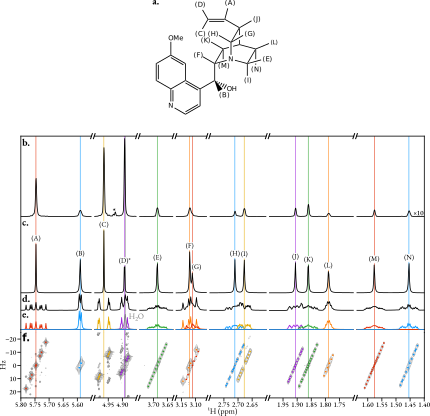
\includegraphics{quinine_cupid/quinine_cupid.pdf}
    \caption[
        Application of \acs{CUPID} on the non-aromatic regions of a quinine
        \acs{2DJ} dataset.
    ]{
        Application of \ac{CUPID} on the non-aromatic regions of a quinine
        \ac{2DJ} dataset.
        \textbf{a.} The spectrum generated from \ac{FT} of the \ang{-45}
        signal, with the green signal arising from water at about
        \qty{4.89}{\partspermillion} neglected.
        \textbf{b.} Conventional \ac{1D} spectrum.
        \textbf{c.} Multiplet structures assigned ($\epsilon =
        \nicefrac{\fswtwo}{\Ntwo} \approx \qty{0.92}{\hertz}$).
        \textbf{d.} Contour plot of the absolute value mode \ac{2DJ} spectrum,
        with the locations of assigned oscillators given as coloured points.
    }
    \label{fig:quinine-cupid}
\end{figure}

Figure \ref{fig:quinine-cupid} illustrates the result of applying \ac{CUPID} on
a dataset generated from a sample comprising quinine in CD\textsubscript{3}OD,
with all non-aromatic protons considered. The method successfully generated a
pure shift spectrum with distinct peaks for each \textsuperscript{1}H
environment. This example also highlights an added benefit of using \ac{CUPID}:
the ability to suppress unwanted signals in the final spectrum. In this
example, an intense, broad singlet at around \qty{4.89}{\partspermillion}
was detected (see the green peak at this frequency in panel c).
The singlet was due to the presence of water in the sample and was a hindrance
due to it overlapping heavily with the multiplet structure corresponding to
spin D. To obtain a clean singlet for spin D in the pure shift spectrum, the
oscillator corresponding to the water signal was simply neglected from
$\bthstar$ in generating the \ang{-45} signal. \note{Find reference for work
talking about using estimation for solvent suppression.}

As eluded to already, a few of the peaks in the pure-shift spectrum are rather
broad on account of the estimation routine under-fitting the relevant multiplet
structure. The most notable example of this phenomenon in the quinine example
comes from the peak for spin G, where siginifcant overlap with spin F has likely
compunded the task of accurately estimating the \ac{FID}. With fewer than the
true number of oscillators fitting a given multiplet structure, the \ac{NLP}
routine will compensate by giving the oscillators it does have at its disposal
large amplitudes and damping factors, so that they can reasonably fit multiple
similar-frequency oscillators.
While affecting peak linewdiths, this feature does not tend to significantly
affect the integrals of the pure shift peaks. \note{Should probably calculate
the integrals of these...}

\subsubsection{Dexamethasone}

\begin{sidewaysfigure}%
    \centering%
    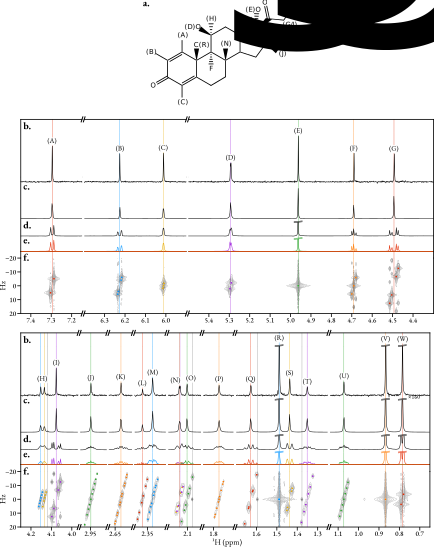
\includegraphics{dexamethasone_cupid/dexamethasone_cupid.pdf}%
    \caption[
        Application of \ac{CUPID} on a dexamethasone dataset.
    ]{
        Application of \ac{CUPID} on dexamethasone \ac{2DJ} dataset.
        \textbf{a.} \ac{TSE-PSYCHE} spectrum of the sample.
        \textbf{b.} The spectrum generated from \ac{FT} of the \ang{-45}
        signal.
        \textbf{c.} Conventional \ac{1D} spectrum.
        \textbf{.} Multiplet structures assigned ($\epsilon =
        \nicefrac{\fswtwo}{\Ntwo} \approx \qty{0.92}{\hertz}$).
        \textbf{d.} Contour plot of the absolute value mode \ac{2DJ} spectrum,
        with the locations of assigned oscillators given as coloured points.
    }
    \label{fig:dexamethasone-cupid}%
\end{sidewaysfigure}%
\note{Double check mp thold}

Figure \ref{fig:dexamethasone-cupid} shows the result of applying CUPID on a
dataset acquired from a sample dexamethasone in DMSO-d\textsubscript{6}. A
pure-shift spectrum was also acquired using the
\ac{TSE-PSYCHE} experiment\cite{Foroozandeh2018,Foroozandeh2015} for
comparison.
\ac{CUPID} generated a pure-shift spectrum with overall excellent agreement
with the PSYCHE spectrum. Certain multiplet structures in the spectrum exhibit
splitting in $\Ftwo$, on account of heteronuclear couplings to \textsuperscript{19}F. Most
notable are those derived from spins D, H \& O. For the D multiplet, the
magnitude of $J_{\textsuperscript{1}H,\textsuperscript{19}F}$ is very small
such that assigning these to separate oscillators is infeasible.
For the spin N multiplet, two separate structures were successfully assigned
(see the orange and green multiplets around \qty{2.1}{\partspermillion}).
The estimation routine was unsuccessful at accurately estimating the structure
associated with spin H, where a severe under-fitting occurred. An under-fitting
of this structure even occurred when the estimation was re-run using
considerable over-estimation of the model order, with most oscillators in the
initial guess being purged during the \ac{NLP} procedure. The result of
under-fitting, as already discussed, leads to peaks in the final \ac{CUPID}
spectrum being broadened, with the spin H multiplet providing an extreme
example of this. The most downfield peaks in the CUPID spectrum (corresponding
to aromatic and hydroxyl protons) also appear to be noticeably broadened
relative to their PSYCHE equivalents. This is also probably due to
under-fitting of the relevant multiplet structures, though to a far less
noticeable extent than for spin H. \note{Any other reason why this might be so?}


\section{Sequential Datasets}
\label{sec}

There are a number of two-dimensional \ac{NMR} experiments in which the
variation of a parameter in the pulse sequence leads to the generation of
\acp{FID} of the same form except for an attenuation in their amplitudes. These
include experiments for the determination of translational diffusion rates and
relaxation properties such as $T_1$, $T_2$, and $T_{1\rho}$. Estimation of such
datasets using nonlinear programming is attractive as after the first \ac{FID}
has been estimated without \textit{a priori} information, subsequent \acp{FID}
can be estimated using the previous result as an initial guess. On top of this,
only the amplitudes of each increment need to be optimised, as the phases,
frequencies and damping factors will be unperturbed across increments.

In this chapter, a generalised approach to analysing such datasets using the
estimation procedure presented in Chapter \ref{chap:theory} is presented.

\subsection{Methodology}

\subsubsection{Outline of the problem}
There are numerous experiments in which the pulse sequence is repeated over
multiple values of a certain parameter $\symbf{v} \in \mathbb{R}^I$. Examples
of this are various relaxation experiments (Section
\ref{sec:relaxation_experiments}) in which this parameter is effectively the
amount of time relaxation is allowed to occur, and diffusion experiments
(Section \ref{sec:diffusion_experiments}) in which it is the strength of the
diffusion-encoding \acp{PFG}. These experiments lead to an FID $\symbf{Y} \in
\mathbb{C}^{I \times N}$ in which the value of the experimental parameter
attenuates the amplitudes of the contributing resonances:
\begin{equation}
    Y[i, n] = \sum_{m=1}^M a_m^{(i)} \exp\left(\iu \phi_m\right)
        \exp\left(\left(2 \pi \iu f_m - \eta_m \right) n \Dt\right).
\end{equation}
The variation of the amplitudes of all resonances is described by the parameter
vector $\symbf{p} \in \mathbb{R}^{2M}$:
\begin{equation}
    \symbf{p} = \left[
        \zeta_1, \psi_1, \zeta_2, \psi_2, \cdots, \zeta_M, \psi_M
    \right]^{\mathrm{T}}.
\end{equation}
$\symbf{\zeta} = \lbrace\zeta_1, \cdots, \zeta_M\rbrace$ are a set of scaling
parameters, one per oscillator, that are not typically of
interest, but that are necessary for extracting  $\symbf{\psi} = \lbrace
\psi_1, \cdots, \psi_M \rbrace$, the of set parameters of interest (relaxation
rates, diffusion rates, etc. associated with each oscillator). The amplitudes
vary from increment to increment as a result of some function $\mathcal{A}$,
whose form varies across different types of experiments (see Table
\ref{tab:seq_equations}). In general:
\begin{equation}
    a^{(i)}_m = a_m(v_i, \zeta_m, \psi_m) = \zeta_m \mathcal{A}\left(v_i, \psi_m \right)
\end{equation}

\begin{table}
    \begin{center}
        \begin{tabular}{ccccccc}
            \hline
            Experiment &
            $v$ &
            $\zeta$ &
            $\psi$ &
            $\mathcal{A}(v, \psi)$ &
            $\frac{\partial \mathcal{A}(v, \psi)}{\partial \psi}$ &
            $\frac{\partial^2 \mathcal{A}(v, \psi)}{\partial \psi^2}$ \\ \hline
            Inversion Recovery &
            $\tau$ &
            $a_{\infty}$ &
            $T_1$ &
            $\left(1 - 2 \exp \left(-\frac{\tau}{T_{1}}\right)\right)$ &
            $-\frac{2 \tau}{T_1^2} \exp\left(-\frac{\tau}{T_1}\right)$ &
            $\frac{2 \tau}{T_1^3} \exp\left(-\frac{\tau}{T_1}\right)\left(2 - \frac{\tau}{T_1}\right)$\\
            CPMG &
            $n_{\textrm{cycles}}$ &
            $a_0$ &
            $T_2$ &
            ? &
            ? &
            ? \\
            Diffusion &
            $g$ &
            $a_0$ &
            $D$ &
            $\exp\left(-c g^2 D\right)$ &
            $-c g^2 \exp\left(-c g^2 D\right)$ &
            $c^2 g^4 \exp\left(-c g^2 D\right)$ \\
            \hline
       \end{tabular}
       \caption{
           The various functional forms of $\mathcal{A}$ according to the
           different sequential NMR experiments considered in this thesis.
           $\mathcal{A}$ describes how the amplitude of a resonance is affected
           by the experimental parameter $v$.
       }
       \label{tab:seq_equations}
    \end{center}
\end{table}

Determination of $\psi_m$, the parameter of interest for a given oscillator can be achieved by nonlinear programming, via optimisation of the fidelity
\begin{subequations}
    \begin{gather}
        \mathcal{F}\left(\zeta_m, \psi_m | \symbf{v}\right) =
            \left \lVert \symbf{a}_m - \zeta_m \mathcal{A} \left(\symbf{v},
            \psi_m\right) \right\rVert_2^2,\\
        \symbf{a} = \left[a_m^{(1)}, a_m^{(2)}, \cdots,
            a_m^{(I)}\right]^{\mathrm{T}}.
    \end{gather}
\end{subequations}

Derivatives:
\begin{subequations}
    \begin{gather}
        \frac{\partial \zeta_m \mathcal{A} \left(v_i, \psi_m\right)}
            {\partial \zeta_m} =
            \mathcal{A}\left(v_i, \psi_m\right) \\
        \frac{\partial \zeta_m \mathcal{A} \left(v_i, \psi_m\right)}
            {\partial \psi_m} =
            \zeta_m \frac{\partial\mathcal{A}\left(v_i, \psi_m\right)}{\partial \psi_m}\\
        \frac{\partial^2 \zeta_m \mathcal{A} \left(v_i, \psi_m\right)}
            {\partial \zeta_m^2} = 0\\
        \frac{\partial^2 \zeta_m \mathcal{A} \left(v_i, \psi_m\right)}
            {\partial \psi_m \partial \zeta_m} =
            \frac{\partial^2 \zeta_m \mathcal{A} \left(v_i, \psi_m\right)}
            {\partial \zeta_m \partial \psi_m} =
            \frac{\partial\mathcal{A}\left(v_i, \psi_m\right)}{\partial \psi_m}\\
        \frac{\partial^2 \zeta_m \mathcal{A} \left(v_i, \psi_m\right)}
            {\partial \psi_m^2} =
            \zeta_m \frac{\partial^2 \mathcal{A}\left(v_i, \psi_m\right)}{\partial \psi_m^2}\\
    \end{gather}
\end{subequations}

It therefore is necessary to determine the amplitudes of a given oscillator for a given increment, which is desribed in the next section

\subsubsection{Determining amplitudes}


\subsection{Relaxation experiments}
\label{sec:relaxation_experiments}

Integrals of peaks modelled with two parameters $\symbf{\theta} \in \mathbb{R}^2$:
\begin{subequations}
   \begin{gather}
        \theta_1 = I_{\infty} = \lim_{\tau \rightarrow \infty} x\\
        \theta_2 = T_1
   \end{gather}
\end{subequations}

\begin{equation}
    \symbf{I}\left(\symbf{\theta}, \symbf{\tau}\right) =
        I_{\infty} \left[ 1 - 2 \exp\left( -\frac{\symbf{\tau}}{T_1}\right) \right],
\end{equation}

Fitting this function is achieved by minimising L2-norm (reference it in
previous discussion, and refer to grad and Hessian). The first and second
derivatives of the model, required to construct the grad and Hess are
\begin{subequations}
    \begin{gather}
        \frac{\partial I}{\partial I_{\infty}} =
            1 - 2 \exp \left( -\frac{\tau}{T_1} \right)\\
        \frac{\partial I}{\partial T_1} =
        -\frac{2 I_{\infty} \tau}{T_1^2} \exp\left( -\frac{\tau}{T_1} \right)\\
        \frac{\partial^2 I}{\partial I_{\infty}^2} = 0\\
        \frac{\partial^2 I}{\partial I_{\infty} \partial T_1} =
            \frac{\partial^2 I}{\partial T_1 \partial I_{\infty}} =
            -\frac{2 \tau}{T_1^2} \exp\left(- \frac{\tau}{T_1} \right)\\
        \frac{\partial^2 I}{\partial T_1^2} =
            \frac{2 I_{\infty} \tau}{T_1^3} \exp\left(- \frac{\tau}{T_1} \right)
            \left(2 - \frac{\tau}{T_1}\right)
    \end{gather}
\end{subequations}

\subsection{Diffusion experiments}
\label{sec:diffusion_experiments}

Along with their widespread use in dephasing undesired coherences in a pulse
sequence, the use of \acp{PFG} is central to determining translational
diffusion properties of species with NMR. The first showcase for extracting
translational diffusion coefficients came from Stejskal and Tanner in 1965, in
which they introduced the \ac{PGSE} pulse sequence\cite{Stejskal1965} (Figure
\ref{fig:diffusion_sequences}.a).

The \ac{PGSE} sequence consists of a conventional spin-echo ($\ang{90}
\xrightarrow{\tau} \ang{180} \xrightarrow{\tau} \text{acquire}$), with
\acp{PFG} applied after each of the \ac{RF} pulses.
As a simple overview of how the pulse sequence works, consider a single spin on
resonance with the transmitter (i.e. its rotating frame frequency is zero) in a
sample tube at position $z$ along the axis collinear with the main field.
After the \ang{90} pulse, the magnetisation will be $-M_y$.
During the first \ac{PFG}, the spin's resonance frequency will become
$\omega_{\text{PFG}} = -\gamma g z$, where $g$ is the strength of the \ac{PFG}.
Assuming the gradient is applied for a time $\delta$, the spin will
precess by an angle of  $\alpha = -\gamma g z \delta$. After the \ang{180}
pulse, the spin's magnetisation is as follows:
\[
    -M_y
    \xrightarrow{\text{PFG}} -M_y \cos(\alpha) + M_x \sin(\alpha)
    \xrightarrow{\ang{180}_y} -M_y \cos(\alpha) - M_x \sin(\alpha).
\]
Supposing that the spin has moved to a new position $z + \Delta_z$
between the end of the first gradient and the beginning of the second,
application of the second gradient causes precession by the angle
$\beta = -\gamma g (z + \Delta_z) \delta$:
\begin{equation*}
   \begin{split}
        \xrightarrow{\text{PFG}}
            &-M_y \cos(\alpha)\cos(\beta) +
            M_x \cos(\alpha)\sin(\beta) -
            M_x \sin(\alpha)\cos(\beta) -
            M_y \sin(\alpha)\sin(\beta)\\
        &= -M_y \cos(\gamma g \delta \Delta_z) -
           M_x \sin(\gamma g \delta \Delta_z),
   \end{split}
\end{equation*}
In the scenario that the spin has not translated in the $z$-direction between
\acp{PFG} ($\Delta_z = 0$), the net effect of the pulse sequence is nothing
(except for a loss of signal amplitude through $T_2$ relaxation). However, if
translation does occur, the signal phase is adjusted, as a function of the
extent of translation $\Delta_z$. The gradients have effectively been employed
to encode the change in position of the spin after a known amount of time.
Extending this idea to a system of many identical spins, which will translate
by different extents between the \acp{PFG}, individual spin contributions to
the bulk magnetisation will become dephased, leading to an attenuation of the
amplitude of the resulting FID.

\begin{figure}
   \includegraphics{diffusion_sequences/diffusion_sequences.pdf}
   \caption[
       Pulse sequences used for the determination of translational diffusion constants.
   ]{
       Pulse sequences used for the determination of translational diffusion constants.
       \textbf{a.} \acs{PGSE},
       \textbf{b.} \acs{PGSTE},
       \textbf{c.} \acs{PGSTEBP},
       \textbf{d.} One-shot DOSY.
       \ac{RF} pulses are denoted by solid rectangles. Diffusion-encoding
       gradients are denoted by sine-bell shapes with varying shades,
       indicating that the intensity is incremented to create a \ac{2D}
       dataset. Spoiler gradients are denoted by solid black sine-bell shapes.
   }
   \label{fig:diffusion_sequences}
\end{figure}

Through consideration of the Bloch-Torrey equations\cite{Torrey1956}, which
extend the classic Bloch equations to account for the effects of diffusion on
magnetisation, Stejskal and Tanner were able to derive the following equation
for the variation of the amplitude of a resonance as a function of gradient
strength, known widely as the Stejskal-Tanner equation:
\begin{equation}
    a(g) = a_0 \exp \left(- \gamma^2 \delta^2 g^2 D \left(\Delta -
    \frac{\delta}{3}\right)\right),
    \label{eq:stejskal_tanner}
\end{equation}
where
$a_0 = \lim_{g \rightarrow 0} a$,
$\gamma$ is the gyromagnetic ratio of the target nucleus
(\unit{\mega\hertz\per\tesla}),
$g$ is the gradient strength (\unit{\tesla\per\meter})\footnote{
    Gradient strengths are often expressed in units of
    \unit{\gauss\per\centi\meter}, which is equivalent to
    \qty[print-unity-mantissa = false]{e-2}{\tesla\per\meter}.
},
$\delta$ is the duration of the \acp{PFG} (\unit{\second}),
$\Delta$ is the delay between the \acp{PFG}, often known as the diffusion time
(\unit{\second}),
and $D$ is the translation diffusion constant of the species giving rise to the
resonance (\unit{\meter\square\per\second}).
While Equation \ref{eq:stejskal_tanner} is widely stated in the literature, it
is only technically applicable to the scenario in which the \ac{PGSE} sequence
is used (or any other \emph{monopolar} sequence, \emph{vide infra}), and
rectangular \acp{PFG} are applied
\footnote{
    Rectangular \acp{PFG} (i.e. those in which there is an infinitesimal time
    to rise to full strength, and to fall back to zero) are in fact
    impossible to achieve as they would require gradient coils with zero
    inductance.
}.

Tanner introduced a variant on the original \ac{PGSE} experiment called
\ac{PGSTE}\cite{Tanner1970} (Figure \ref{fig:diffusion_sequences}.b). Instead
of the diffusion period including a
\ang{180} pulse, \ac{PGSTE} has two \ang{90} pulses, with the first being
applied shortly after the initial \ac{PFG}, and the second being applied just
before the second \ac{PFG}. The key difference between this and the \ac{PGSE}
experiment is that relaxation of the signal during the diffusion time is
dictated by longitudinal relaxation ($T_1$), rather than transverse relaxation
($T_2$). \ac{PGSTE} is therefore favoured in scenarios where $T_1 \ll T_2$, as
improved sensitivity will be achieved in the resulting \ac{FID}.


Both \ac{PGSE} and \ac{PGSTE} employ \emph{monopolar} \acp{PFG} for diffusion
encoding, in the sense that they are both polarised in a
single direction. Experiments also exist which employ
\emph{bipolar} gradient elements\cite{Cotts1989,Wu1995}, which consist of a
\ac{PFG}, followed by a \ang{180} pulse, and then a second \ac{PFG} with the
opposite polarity to the first. A well-known example is the \ac{PGSTEBP}
experiment (Figure \ref{fig:diffusion_sequences}.c). Bipolar gradient are
useful in circumstances where it is important to purge the effects of static
gradients in the sample, caused by field inhomogeneities. Morris and coworkers
have also developed the One-shot DOSY experiment\cite{Pelta2002} (Figure
\ref{fig:diffusion_sequences}.d), which requires a single transient per
gradient strength (i.e. there is no requirement for a phase-cycling scheme).
This is achieved through the use of bipolar gradients which comprise
asymmetrical \acp{PFG} with relative powers $1 + \alpha : 1 - \alpha$ for some
$\alpha > 0$
\footnote{
    $\alpha$ is typically set to be considerably less that $1$, commonly $0.2$.
}.
\note{Cite some review articles (Johnson, Morris 2009)}

It is virtually always the case that the amplitudes of each resonance in the
\ac{FID} abide by the following general form of the Stejskal-Tanner equation:
\begin{equation}
    a(g) = a_0 \exp\left(- c g^2 D\right)
\end{equation}
for some constant $c$ (\unit{\tesla\per\second\squared}).
It is important to note that functional form of $c$ is highly variable
dependent on the type of experiment used, and its value if affected by the
shape of the diffusion-encoding \acp{PFG}. A consideration of the Bloch-Torrey
equation for a given experiment is necessary, with an extensive overview
provided by Sinnaeve for most diffusion NMR experiments\cite{Sinnaeve2012}. In
general, $c$ is as follows:
\begin{equation}
    c = \gamma^2 \delta^2 \sigma^2 \Delta^{\prime}.
    \label{eq:stejskal_tanner_generic}
\end{equation}
$\sigma$ is the \emph{shape factor} of the \acp{PFG} (\emph{vide infra}), and
$\Delta^{\prime}$ is the effective time that diffusion is allowed to occur.
Examples of the value of $\Delta^{\prime}$ include:
\begin{subequations}
    \begin{alignat}{2}
        & \text{Monopolar gradients (\ac{PGSE}, \ac{PGSTE})} \quad && \Delta + 2 \left(\kappa - \lambda\right) \delta,
        \label{eq:monopolar}\\
        & \text{Bipolar gradients (\ac{PGSTEBP})} \quad && \Delta + \frac{\left(2 \kappa - 2 \lambda
            - 1\right)\delta}{4} - \frac{\tau}{2},\\
        & \text{One-shot}
            \quad && \Delta + \frac{\left(\kappa - \lambda\right)
            \left(\alpha^2 + 1\right) \delta}{2} +
            \frac{\left(\delta + 2 \tau\right)\left(\alpha^2 - 1\right)}{4}.
    \end{alignat}
\end{subequations}
$\tau$ is the delay between the initial \ac{PFG} and the \ang{180} pulse in
experiments with bipolar gradients.
The factors $\sigma$,  $\lambda$, and $\kappa$ are related to the shape
function $s(\epsilon) : \epsilon \in [0, 1]$ of the \ac{PFG}, which describes
the variation in the intensity of the gradient as a function of its progression.
For a rectangular gradient, $s(\epsilon) = 1 \forall \epsilon$, whereas for a
sine-bell gradient, $s(\epsilon) = \sin(\pi \epsilon)$. The cumulative
distribution of the shape function is given by:
\begin{equation}
    S(\epsilon) = \int_0^{\epsilon} s\left(\epsilon^{\prime}\right)
            \mathrm{d} \epsilon^{\prime} \quad \forall \epsilon \in [0, 1].
\end{equation}
The corresponding definition of $S$ for the case of a gradient made of discrete
steps with shape function $\symbf{s} \in \mathbb{R}^{N_g}$ is
\begin{equation}
    S\left[n\right] =
        \frac{1}{n} \sum_{i = 0}^{n} s\left[i\right] \quad
        \forall n \in \left\lbrace 0, \cdots, N_g - 1\right\rbrace,
\end{equation}
where $N_g$ is the number of points the gradient comprises. The three factors
are given by
\begin{subequations}
    \begin{gather}
        \sigma = S(1),\\
        \lambda = \frac{1}{\sigma} \int_0^1 S(\epsilon) \mathrm{d} \epsilon,\\
        \kappa = \frac{1}{\sigma^2} \int_0^1 S^2(\epsilon) \mathrm{d} \epsilon,
    \end{gather}
\end{subequations}
with their discrete counterparts being
\begin{subequations}
    \begin{gather}
        \sigma = S\left[N_g - 1\right] \\
        \lambda = \frac{1}{\sigma N_g} \sum_{n = 0}^{N_g - 1} S\left[n\right]
            = \frac{1}{\sigma N_g} \sum_{n = 0}^{N_g - 1}
            \frac{1}{n} \sum_{i=0}^{n} s\left[i\right]\\
        \kappa = \frac{1}{\sigma^2 N_g} \sum_{n = 0}^{N_g - 1} S^2\left[n\right]
            = \frac{1}{\sigma^2 N_g} \sum_{n = 0}^{N_g - 1}
            \frac{1}{n^2} \left(\sum_{i=0}^{n} s\left[i\right]\right)^2
    \end{gather}
\end{subequations}
For \acp{PFG} with a symmetrical shape, $\lambda = \nicefrac{1}{2}$. $\kappa$
is typically equal to or close to $\nicefrac{1}{3}$. It can now be seen that
Equation \ref{eq:stejskal_tanner} comes from plugging Equation
\ref{eq:monopolar} into Equation \ref{eq:stejskal_tanner_generic}, with $\sigma
= 1$,  $\lambda = \nicefrac{1}{2}$, and  $\kappa = \frac{1}{3}$. In many
situations,  $\Delta$ dominates in the expression of $\Delta^{\prime}$, and so
ensuring the correct form of $c$ could be seen as excessive. However,
especially when  $\Delta$ is not orders of magnitude greater than $\delta$, the
exact form of $\Delta^{\prime}$ used in Equation
\ref{eq:stejskal_tanner_generic} will be extremely important for accurate
measurements of $D$.

The necessary first and second derivatives required to estimate the translational diffusion constant using the \ac{Trust NCG} algorithm are:
\begin{subequations}
   \begin{gather}
       \frac{\partial a}{\partial a_0} = \exp\left(-c g^2 D\right) \\
       \frac{\partial a}{\partial D} = -a_0 c g^2 \exp\left(-c g^2 D\right) \\
       \frac{\partial^2 a}{\partial a_0^2} = 0\\
       \frac{\partial^2 a}{\partial a_0 \partial D} =
           \frac{\partial^2 a}{\partial D \partial a_0} =
           -c g^2 \exp\left(-c g^2 D\right) \\
       \frac{\partial^ 2 a}{\partial D^2} = a_0 c^2 g^4 \exp\left(-c g^2 D\right)
   \end{gather}
\end{subequations}

\begin{equation}
    \frac{\partial^n x}{\partial D^n} = \left(-c G^2\right)^n \exp\left(-c D G^2\right)
\end{equation}

\subsection{Plotting DOSY-type results}
Spectrum $S \in \mathbb{R}^{N, I}$ is given by
\begin{subequations}
    \begin{gather}
        S = \sum_{m=1}^M \symbf{s}_m \otimes \frac{\symbf{d}}{\max\left(\symbf{d}\right)} \\
        \symbf{s}_m = \FT\left\lbrace
            a^{(1)}_m \exp\left(\iu \phi_m\right) \exp\left(\left(2 \pi \iu f_m - \eta_m\right) \symbf{n} \Dt\right)
        \right\rbrace \\
        \symbf{d}  = \exp\left(
            -\frac{\left(\symbf{y} - \theta_2\right)^2}
            {2 \sigma_2^2}
        \right)
    \end{gather}
\end{subequations}

\section{Phased broadband spectra from single chirp excitation}
\label{sec:bbqchili}

The are numerous nuclei of considerable interest to \ac{NMR} practitioners with
very wide chemical shift ranges, including \textsuperscript{13}C,
\textsuperscript{19}F -- of particular interest in the
pharmaceutical industry -- and \textsuperscript{31}P. Attaining spectra
covering the entire
chemical shift range of such spins for use in quantitative applications is
challenging due to off-resonance effects, which severely alter the amplitudes
and phases of resonances with frequencies far from the transmitter
frequency\cite[Section 3.4.1]{Cavanagh2007}. One popular means of achieving
\emph{broadband} excitation, in which a consistent amplitude- and phase-profile
across the spectral window the achieved, is to use swept-frequency (chirp)
pulses, whose excitation frequency varies with
time\cite{Bohlen1989,Bohlen1993}.
The application of a single \ang{90} chirp pulse to achieve broadband
excitation, while simple, yields spectra with undesirable phase behaviour, on
account of resonances with different frequencies being excited at different
moments during chirp application. However, with knowledge of the form of the
chirp pulse, the expected phase of a particular resonance is determinable, and
can be corrected with appropriate post-processing.

In this section, a description of a method given the name \ac{BBQCHILI} is
presented, which provides a means of acquiring well-phased broadband spectra
from single chirp excitation. \ac{BBQCHILI} comprises two key steps: (a)
estimation of the acquired \ac{FID}'s parameters, (b) generation of a synthetic
\ac{FID}, with each contributing oscillator being back-propagated by an
appropriate amount, according to its resonance frequency. A description of the
technique is presented, followed by an illustration of its performance on
simulated and experimental datasets.

\subsection{An overview of single chirp excitation}
Here, focus is limited to chirp pulses whose frequency varies linearly with
time, which sweep from low to high frequencies. Such a pulse is defined by its
duration $\tau_{\text{p}}$ (\unit{\second}),
excitation bandwidth $\Updelta F$ (\unit{\hertz}),
and \ac{RF} amplitude $\nu_{\text{RF}}$ (\unit{\hertz}).
The frequencies that the pulse sweeps through are in the range $\left[\foffone -
\nicefrac{1}{2} \Updelta F, \foffone + \nicefrac{1}{2} \Updelta F\right]$, and
the rate at which the frequency of the chirp is increased (the sweep rate) is
given by $\nicefrac{\Updelta F}{\tau_{\text{p}}}$.
Figure \ref{fig:single-chirp} provides an illustration of a single chirp
excitation experiment. After application of the chirp pulse, there is commonly
a short \emph{pre-scan delay} $\tau_{\text{del}}$, typically on the order of
\unit{\micro\second}, prior to the start of acquisition, which is also of
relevance in order to process the \ac{FID}.

The various pulse parameters are inter-related as follows:
\begin{equation}
    \nu_{\text{RF}} = \sqrt{
        \frac{\Updelta F Q}{2 \pi \tau_{\text{p}}}
    },
\end{equation}
where $Q \in \mathbb{R}_{>0}$ is the \emph{adiabaticity factor} \note{More
detail/citation?}. For a pulse with flip angle  $\beta < \ang{180}$,  $Q$ is
related to $\beta$ via
\begin{equation}
    Q = \frac{2}{\pi} \ln \left( \frac{2}{\cos(\beta) + 1} \right),
\end{equation}
\note{ref?}
such that an appropriate pulse to achieve a flip angle of \ang{90} requires
selecting a combination of $\nu_{\text{RF}}$, $\Updelta F$, and
$\tau_{\text{p}}$ which satisfies $Q \approx 0.441$.

\begin{figure}
    \centering
    \includegraphics{single_chirp_illustration/single_chirp_illustration.pdf}
    \caption[
        An illustration of an experiment comprising a single chirp pulse.
    ]
    {
        An illustration of an experiment comprising a single chirp pulse sweeping
        low to high frequencies of duration $\tau_{\text{p}}$, followed by
        a pre-scan delay period or $\tau_{\text{del}}$, prior to
        acquisition. The fate of three resonances with different frequencies is
        denoted, with $\fone_{\text{red}} < \fone_{\text{blue}} <
        \fone_{\text{yellow}}$. Each resonance is excited at different points
        in time, with lower frequency resonances being excited earlier, such that
        each resonance is allowed to evolve for different amounts of time prior
        to acquisition ($t_0$).
        The resulting \ac{FID} possesses quadratic phase behaviour.
        Coloured oscillations denote the evolution of each resonance, with
        solid and dashed lines representing real and imaginary components,
        respectively. It is assumed that the \ang{90} chirp rotates each
        resonance to be initially in phase with the receiver.
    }
    \label{fig:single-chirp}
\end{figure}

For a pulse with sufficiently low $\nu_{\text{RF}}$ (which in turn requires a
sufficiently large $\tau_{\text{p}}$ for a given excitation bandwidth) it is
valid to assume that the chirp induces an instantaneous \ang{90} rotation
of a spin at the point of resonance. As such, resonances with different
frequencies evolve for different amounts of time prior to the start of
acquisition, according to
\begin{equation}
    t_0\left( \fone \right) =
        \tau_{\text{del}} + \frac{\tau_{\text{p}}}{2} -
        \frac{\left( \fone - \foffone \right) \tau_{\text{p}}}{2 \Updelta F}.
    \label{eq:t0}
\end{equation}
$\tau_{\text{del}} + \nicefrac{1}{2} \tau_{\text{p}}$ is the amount of time
between excitation and detection for an on-resonance oscillator. Resonances
with an frequency smaller than the transmitter are excited earlier and hence
have a larger $t_0$, while the converse is true for resonances with greater
frequencies. An illustration of this phenomenon is provided by Figure
\ref{fig:single-chirp}.

\subsection{Quadratic phase correction and \acs{BBQCHILI}}
Appropriate phasing of the spectrum generated via single chirp excitation can
be reduced to a trivial zero-order problem by applying phase correction
(Section \ref{subsec:nmr-analysis}), with \note{Check $2 \pi$}
\begin{equation}
    \phi \left( \fone \right) =
        \underbrace{
            2 \pi \left(\fone - \foffone\right) \left(\tau_{\text{del}}
            + \frac{\tau_{\text{p}}}{2} \right)
        }_{\phi_1} -
        \underbrace{
            2 \pi \left(\fone - \foffone\right)^2 \left(
            \frac{\tau_{\text{p}}}{2 \Updelta F} \right)
        }_{\phi_2}.
    \label{eq:quadratic-phase}
\end{equation}
While \eqref{eq:quadratic-phase} is able to correct the quadratic phase
behaviour of peaks, it is unable to address another issue with the dataset,
which is the fact that for each resonance, a number of initial points are not
present in the \ac{FID}.
For any resonance, the signal that is actually detected can be thought of as
the difference between two signals: (a) the ``complete'' signal, which starts
at the time of excitation, and (b) a ``truncated'' signal which is identical to
the complete signal before acquisition, and which comprises zeros once
acquisition has begun. The linear nature of the \ac{FT} dictates that the
resulting delayed-acquisition spectrum comprises the difference between the
\acp{FT} of the complete signal and the truncated signal.  The \ac{FT} of the
truncated \ac{FID} is well approximated as a broad sinc wiggle with its maximum
at the resonance frequency. The form of the wiggle depends on the delay between
excitation and acquisition, with resonances of lower frequencies, for which
more of the signal is missed, displaying deeper, and narrower artefacts. The
result of applying quadratic phase correction is therefore a spectrum of
well-phased peaks, but with severe baseline distortion, particularly to the
right-hand (low frequency) end. Panel b of Figure
\ref{fig:chirp-phase-vs-backprop} provides an example of this phenomenon.

Both quadratic phase and missing point-derived baseline distortions can be
resolved if an estimate of the \acp{FID} parameters is obtained. Estimation
opens up the means of constructing \iac{FID} featuring oscillators which
are back-propagated, such that they begin not at the point of acquisition, but
at the point of excitation. The appropriate start time for an oscillator with
frequency $\fone$ is therefore given by $-t_0\left( \fone \right)$, with  $t_0$
defined in \eqref{eq:t0}. The resulting corrected \ac{FID} $\by_{\text{corr}}$
is as follows:
\begin{equation}
    \begin{split}
        \by_{\text{corr}} \left[ \none \right] =
            &\sum_{m=0}^{M-1} \bdam \exp \left( \iu \bdphim \right) \times \\
            &\exp\left(-
            \left(2 \pi \iu \left(\bdfonem - \foffone \right) - \bdetaonem \right)
            t_0 \left(\bdfonem\right) \none \Dtone
            \right).
    \end{split}
\end{equation}
Estimation can be carried out using the \ac{MPM}, with the option of applying
\ac{NLP} afterwards. However, the variance of oscillator phases should not be
included in the fidelity for \ac{NLP}, since the phases in the dataset are
quadratically distributed. For the examples presented in this work, the direct
output of the \ac{MPM} was used.

\begin{figure}
    \centering
    \includegraphics{chirp_phase_vs_estimation/chirp_phase_vs_estimation.pdf}
    \caption[
        Comparison of quadratic phase correction vs frequency-dependent
        back-propagation in treating data derived from a single-chirp
        excitation experiment.
    ]
    {
        Comparison of quadratic phase correction vs frequency-dependent
        back-propagation in treating data derived from a single chirp
        excitation experiment.
        \textbf{a.} Simulated spectrum for a spin system comprising 30 spins
        with uniformly-separated resonance frequencies. The data was generated
        with
        $\None=2^{15}$,
        $\fswone=\qty{500}{\kilo\hertz}$,
        $\foffone=\qty{0}{\hertz}$,
        $\tau_{\text{p}} = \qty{100}{\micro\second}$,
        $\tau_{\text{del}} = \qty{6.5}{\micro\second}$,
        $\Updelta F = \qty{500}{\kilo\hertz}$.
        \textbf{b.} Spectrum generated using quadratic phase correction, with
        \eqref{eq:quadratic-phase}.
        \textbf{c.} Spectrum generated from estimation using the \ac{MPM}, and
        back-propagation.
    }
    \label{fig:chirp-phase-vs-backprop}
\end{figure}
Figure \ref{fig:chirp-phase-vs-backprop} provides an illustration of both
quadratic phase correction and the \ac{BBQCHILI} procedure, on a simulated
dataset comprising 30 evenly-separated isolated spins.


\note{Waitng for Ali for response about Gd-doped water data.}


\chapter{The \textsc{NMR-EsPy} Package}
\label{chap:nmrespy}

The estimation routine and applications emerging from it that have been
presented in the previous two chapters are accessible via the \ac{EsPy}
package. \ac{EsPy} aims to provide a feature-rich yet simple interface in order
perform estimation on datasets of interest. In this chapter, a description of
the package is given, including the design choices, a basic description of the
package structure, and a description of the accompanying \ac{GUI}.

A rigorous description of the usage of \ac{EsPy}, including details on
installation, walkthroughs for different data types, and a reference for the
\ac{API} are given in the documentation for \ac{EsPy}. A hard-copy of the
version 2.0 documentation can be found in Section \note{TODO} of the Appendix.
The most up-to-date HTML version of the documentation can be found at
\url{https://foroozandehgroup.github.io/NMR-EsPy/}.
The source code for \ac{EsPy} is hosted on the Foroozandeh group's GitHub page at
\url{https://github.com/foroozandehgroup/NMR-EsPy}.

\section{The Structure of \acs{EsPy}}

\subsection{Why \textsc{Python}?}
There a number of reasons why \textsc{Python} was the chosen programming
language for \ac{EsPy}:
\begin{itemize}
    \item It has a large user-base, particularly within the scientific
        community.
    \item The \textsc{SciPy} ecosystem\cite{Virtanen2020}, including the packages
        \textsc{NumPy}\cite{Harris2020} and
        \textsc{Matplotlib}\cite{Hunter2007} is a powerful tool which enables
        high-performance scientific computation in \textsc{Python}
    \item Being a scripting language makes \textsc{Python} ideal for
        exploring datasets in a step-by-step fashion. This is useful in the
        context of \ac{NMR} estimation, as the user may want to
        (a) inspect and pre-process then data, ten (b) determine the regions
        they wish to estimate, then (c) setup the estimation routine, and
        finally (d) output the estimation result. This can be achieved rather
        easily by hacking and re-running \textsc{Python} scripts or by using
        ``notebook'' environments, such as \textsc{Jupyter}.
    \item It is free and open-source, as opposed to well-known scientific
        computing platforms such as \textsc{Matlab}\textregistered\ and
        \textsc{Mathematica}.
    \item \textsc{Python} supports sophisticated object-oriented programming
        features, such as multiple levels of inheritance.
\end{itemize}

Probably the biggest drawback of \textsc{Python} is its slow performance on
account of it being an interpreted\footnote{
    With interpreted languages, the source code is processed line-by-line at
    the time of running by an interpreter. This differs from compiled
    languages, where prior to being run, the source code is converted to
    machine-readable byte-code.
}
, dynamically typed\footnote{
    Dynamically typed languages, as opposed to statically typed languages like
    \textsc{C}, \textsc{C++}, \textsc{Java}, \textsc{Rust} etc. allow for a
    variable which is initially assigned a given type to be re-assigned to a
    completely different type.
}, language with relies on garbage collection\footnote{
    Garbage collection involves a program routinely checking for any memory
    that has become dereferenced, and clearing this memory up.
}
for memory management. While \textsc{NumPy} provides interfaces to run fast
computations with pre-compiled C-code, a significant performnace benefit would
likely be realised if a low-level compiled language like C, C++, or
\textsc{Rust} were used. However the development time in writing programs with
these lower-level languages is typically a lot greater than with a language
with a higher level of abstraction like \textsc{Python}.

\subsection{???}
The fundamental user-facing object that \ac{EsPy} provides is the
\texttt{Estimator} class and its numerous inherited classes, which facilitate
the estimation of different types of \ac{NMR} data. A
complete list of estimator objects at the time of writing is given in Table
\ref{tab:estimators}

\begin{longtable}{c p{9cm}}
\caption[
    A complete list of estimator objects provided by \ac{EsPy} at the time of writing.
]{
    A complete list of estimator objects provided by \ac{EsPy} at the time of writing.
    \note{Maybe indicate that the inv rec and diffusion estimators share
    similar functionality, except for the amplitude fitting. Diffusion
experiments only differ in definition of fitting constant.}
}
\label{tab:estimators}\\
\hline
Type & Description \\
\hline
\texttt{Estimator1D} & For consideration of 1D datasets. \\
\texttt{Estimator2D} & For consideration of 2D datasets comprising a pair of
States (amplitude-modulated) signals. \\
\texttt{Estimator2DJ} & For consideration of \ac{2DJ} datasets. This object
provides the functionality to generate pure shift spectra and assign multiplet
structures using \ac{CUPID}.\\
\texttt{EstimatorInvRec} & For consideration of inversion recovery ($T_1$)
experiments. \\
\texttt{EstimatorDiffusionMonopolar} & For consideration of monopolar gradient
diffusion experiments. \\
\texttt{EstimatorDiffusionBipolar} & For consideration of bipolar gradient
diffusion experiments. \\
\texttt{EstimatorDiffusionOneshot} & For consideration of one-shot \ac{DOSY}
experiments. \\
\hline
\end{longtable}


\input{text/main/5_conclusions}
\printbibliography
\appendix
\renewcommand{\thealgorithm}{A\arabic{algorithm}}
\renewcommand{\thefigure}{A\arabic{figure}}
\renewcommand{\thetable}{A\arabic{table}}
\setcounter{algorithm}{0}
\setcounter{figure}{0}
\setcounter{table}{0}
\input{text/appendix/data_info.tex}
\input{text/appendix/algorithms}
\section{Structures}

\begin{figure}[h!]
    \centering
    
\includegraphics{structures/structures_final.pdf}
    \caption[
        The molecular structures of species giving rise to the experimental
        \acs{NMR} datasets considered in this work.
    ]{
        The molecular structures of species giving rise to the experimental
        \acs{NMR} datasets considered in this work.
        \textbf{a.} Quinine,
        \textbf{b.} Dexamethasone,
        \textbf{c.} Camphor,
        \textbf{d.} 17\textbeta-estradiol,
        \textbf{e.} Andrographolide.
        Proton environments giving rise to signals which are considered in this
        work are denoted with bracketed alphabetical characters. Non-bracketed
        alphabetical characters denote chemical symbols. \ch{Me} denotes the methyl
        group, equivalent to \ch{CH3}.
        \note{
            TODO: check assignments (esp. estradiol). If more structures need
            adding, edit the ChemDraw file on Chive called
            \path{simon_stuff/thesis_structures.cdxml}. Use EB-Garamond for
            atom labels. One a structure is made, scale to 75\% of original
            size, and set font to 7pt. Then in inkscape, rescale this by
            multiplying by 0.8.
        }
    }
    \label{fig:structures}
\end{figure}

\chapter{Miscellaneous Topics of Interest}
\label{chap:misc}

\subsection{The Nyquist Frequency}
\label{sec:nyquist}
The Nyquist frequency defines the highest frequency an oscillator can possess
such that it is sampled at least twice per period:
\begin{equation}
  f_{\mathrm{N}} = \frac{1}{2\Delta t}
\end{equation}
This quantity as at the heart of the Nyquist-Shannon Sampling Theorem, which -
in the words of Claude Shannon\cite{Shannon1949} - states:
\begin{quote}
  If a function $y(t)$ contains no frequencies
  higher than $f \si{\hertz}$, it is completely determined by giving
  its ordinates at a series of points spaced $\nicefrac{1}{2f}$ seconds
  apart.
\end{quote}
The implication of this is that the continuous FID $y(t)$ may be completely
described by its digitisation with sampling interval $\Delta t$ so long as the
frequencies $f_j$ that make it up satisfy:
\begin{equation}
  \label{permitted_freq}
  -\frac{1}{2\Delta t} \leq f_j \leq \frac{1}{2\Delta t}\ \forall j
\end{equation}
If any frequency $f_j$ does not satisfy \eqref{eq:permitted_freq}, the signal
will be insufficiently sampled, and will be spuriously represented as having a
frequency $f_a$ that satisfies
\begin{alignat}{2}
  &f_a = 2mf_{\mathrm{N}} - f_j \quad \quad &&(f_j > f_{\mathrm{N}})\\
  &f_a = 2mf_{\mathrm{N}} + f_j \quad \quad &&(f_j < -f_{\mathrm{N}}),
\end{alignat}
where $m \in \mathbb{Z}_+$. This phenomenon is called \textit{aliasing}.

\subsection{Hessian Validation}
\note{Talk about checking that my Hessian code is correct by using the finite difference method}

\subsection{Statistical Definitions}
\note{Definitions of standard error, likelihood function, ...}

% \chapter{NMR-EsPy walkthroughs}
The remainder of this thesis is an insert from the documentation of
version 2.0 of \acs{EsPy}. The section of the documentation included provides
walkthroughs describing how to use the package's \ac{API} for the consideration
of \ac{1D} and \ac{2DJ} \ac{NMR} datasets \note{Sequential data too?}. These
walkthroughs provide a short description of the key features associated with
the package, and is an ideal first place to get up-and-running with using it.

Also included in the full documentation are instructions on installation
and using the \acp{GUI} for \ac{1D} and \ac{2DJ} estimation, and a complete
reference for the complete \ac{API}. The most up-to-date version of the
documentation can be found at:
\begin{itemize}
    \item[] \textbf{HTML:} \url{https://foroozandehgroup.github.io/NMR-EsPy/}
    \item[] \textbf{PDF:} \note{???}
\end{itemize}
The source code for \ac{EsPy} is hosted on the Foroozandeh group's GitHub page
at \url{https://github.com/foroozandehgroup/NMR-EsPy}.

\phantomsection
\stepcounter{section}
\addcontentsline{toc}{section}{\protect\numberline{\thesection}1D Walkthrough}
\sectionmark{1D Walkthrough}
\includepdf[%
    pages={13-19},%
    pagecommand={\thispagestyle{fancy}},%
    offset=0 -1cm,%
]{nmr-espy.pdf}

\phantomsection
\stepcounter{section}
\addcontentsline{toc}{section}{\protect\numberline{\thesection}2DJ Walkthrough}
\sectionmark{2DJ Walkthrough}
\includepdf[%
    pages={20-28},%
    pagecommand={\thispagestyle{fancy}},%
    offset=0 -1cm,%
]{nmr-espy.pdf}

\end{document}
